\documentclass[a4paper]{report}
\usepackage[utf8]{inputenc}
\usepackage[T1]{fontenc}
\usepackage{RJournal}
\usepackage{amsmath,amssymb,array}
\usepackage{booktabs}

%% load any required packages FOLLOWING this line
\usepackage{float}
\usepackage[titletoc]{appendix}
\usepackage{adjustbox}
\usepackage{makecell}
\usepackage{hyperref}

\newtheorem{definition}{Definition}
\newcommand{\cK}{\mathcal{K}}
\newcommand{\argmax}{\operatornamewithlimits{argmax}}
\newcommand{\hF}{\widehat{F}}
\newcommand{\tF}{\widetilde{F}}
\definecolor{cornellred}{rgb}{0.7, 0.11, 0.11}
\newcommand{\mycolor}{\color{black}}
\newcommand{\bk}{\color{black}}
\def\rot{\rotatebox}

\begin{document}

%% do not edit, for illustration only
\sectionhead{Contributed research article}
\volume{13}
\volnumber{1}
\year{2021}
\month{June}
\setcounter{page}{493}

%% replace RJtemplate with your article
\begin{article}
  % !TeX root = RJwrapper.tex
\title{\pkg{gofCopula}: Goodness-of-Fit Tests for Copulae}
\author{by Ostap Okhrin, Simon Trimborn and Martin Waltz}

\maketitle

\abstract{
The last decades show an increased interest in modeling various types of data through copulae. Different copula models have been developed, which lead to the challenge of finding the best fitting model for a particular dataset. From the other side, a strand of literature developed a list of different Goodness-of-Fit (GoF) tests with different powers under different conditions. The usual practice is the selection of the best copula via the $p$-value of the GoF test. Although this method is not purely correct due to the fact that non-rejection does not imply acception, this strategy is favored by practitioners. 
Unfortunately, different GoF tests often provide contradicting outputs. The proposed R-package brings under one umbrella \mycolor 13 most used copulae - plus their rotated variants - together with 16 GoF tests and a hybrid one. The package offers \bk flexible margin modeling, automatized parallelization, parameter estimation, as well as a user-friendly interface, and pleasant visualizations of the results. To illustrate the functionality of the package, \mycolor two exemplary applications are provided.\bk
}

\section[Introduction]{Introduction}\label{sec:Intro}
Being firstly introduced in 1959 by Abe Sklar (see \citet{sklar_1959}), copulae gained enormous popularity in applications in the last two decades. Researchers from different fields recognize the power of copulae while working with multivariate datasets from insurance \citep{insurance_paper_1, insurance_paper_2}, finance \citep{finance_paper_1, finance_paper_2}, biology \citep{biology_paper_1, biology_paper_2}, hydrology \citep{hydrology_paper_1, hydrology_paper_2}, medicine \citep{medicine_paper_1, medicine_paper_2}, traffic engineering, \citep{traffic_paper_1, traffic_paper_2}, etc. \mycolor For a recent review, we refer to \cite{grosser2021copulae}. \bk Unfortunately, the correct specification of the multivariate distribution is not easy to find, and often interest in the understanding of the functional form of the copula is dominated by the expected performance of the whole model. This is natural, taking into account the huge list of different copula models proposed in the literature for different needs; see, e.g., \citet{durante2010copula}, \citet{joe2011dependence}, or \citet{genest2014copulas}. Although an expanding list of R-packages devoted to copulae is existent, the issue of GoF testing is less frequently addressed. Primarily, GoF tests for copulae are implemented in copula comparison packages as \CRANpkg{copula} \citep{yan2007enjoy}, \CRANpkg{TwoCop} \citep{TwoCop}, and \CRANpkg{VineCopula} \citep{schepsmeier2018package}, but since \citet{remillard_scaillet_2009} and \citet{genest_remillard_beaudoin_2009}, many other powerful tests were developed that are not integrated into these packages. Most of the tests focus on the bivariate case, leaving a further gap in the existing R-package landscape.

Given a variety of tests, the selection of the most appropriate copula seems \mycolor simple at first glance. \bk However, the power of these tests varies significantly depending on the use case and the copula tested for. The absence of the overall best GoF test leads researchers and practitioners often to the selection of the test (and copula), which supports some subjective expectation, but not the copula that fits the data at its best. Although GoF tests are not intended for model selection but rather to decide whether the selected copula is \emph{not} suitable for the data, the model selection strategy based on the rank of the $p$-values is still commonly used. Following proper scoring rules \citep{gneiting2007strictly}, some tests still allow for selection, and even if not purely statistically sound, it is heavily advocated among practitioners; see \citet{de2014common}. An eloquent illustrative example of different powers and contradictory decisions was provided in \citet{zhang_okhrin_song_zhou_2016}, where three different tests ($R_n$ by \citet{zhang_okhrin_song_zhou_2016}, $S_n$ by \citet{genest_remillard_beaudoin_2009}, and $J_n$ by \citet{scaillet_2007}) were applied for testing the dependency between the standardized returns of the Bank of America and Citigroup. The model selection was done from three copula models: normal, Gumbel, and $t$-copula, based on their respective $p$-values. Interestingly,
\begin{itemize}
    \item[1)] for the year 2004, the $R_n$ gave a favor for the Gumbel copula, while the $S_n$ and $J_n$ for the normal one;
    \item[2)] for the year 2006, the $S_n$ gave the favor for the normal copula, while $R_n$ and $J_n$ for the $t$-copula;
    \item[3)] for the year 2009, the $J_n$ indicated that the dependency is close to the normal one, while $R_n$ and $S_n$ were in favor of the Gumbel copula.
\end{itemize}
This implies that for each year, a \emph{different} pair of tests returns consistent results. In an empirical study, it is difficult to decide which \emph{copula} is suitable and which \emph{test} provides the most plausible results. An extensive comparative study of different GoF tests was performed a decade ago by \citet{genest_remillard_beaudoin_2009}, intensively discussing all, up to that moment existing, tests for copulae. The main findings are that there is no superior blanket test, but several tests have very good power under different, often disjunct conditions.~A test proposed by \citet{zhang_okhrin_song_zhou_2016} fills some gaps in the set of models under which this test performs better than others under certain conditions. However, a common phenomenon in empirical studies is the interpretation of the non-rejection of a copula as the correct model. Especially, in situations where the used GoF test has low power, this is not necessarily the case. Tackling this issue, \citet{zhang_okhrin_song_zhou_2016} also developed the hybrid test, which is simple in construction and implementation. It combines the power of different tests and is very helpful for practitioners; see Section \ref{sec:application}. However, even in this case, the interpretation of finding the \emph{correct} copula should be treated with care.

\mycolor
We propose the R-package \CRANpkg{gofCopula} to automatize the whole empirical procedure of selecting the most suitable copula. Table \ref{tab:Combs_tests_cops_dims} displays the broad range of available tests, copula models, and the maximum dimension. The latest version of this table is also accessible via the function \code{CopulaTestTable()} in the package. Further details on the functionality of each test are provided in Section \ref{sec:gof}, while Table \ref{tbl:copula_characteristics} of Appendix \hyperref[sec:Appendix:cop]{A} contains some characteristics of the copulae implemented in the package.

\begin{table}[H]
\mycolor
\centering
 \begin{adjustbox}{max width=\textwidth}
\begin{tabular}{lcccccccccccccc}
\toprule
Test & \rot{90}{\code{normal}} & \rot{90}{\code{t}} & \rot{90}{\code{clayton}} & \rot{90}{\code{gumbel}} & \rot{90}{\code{frank}} & \rot{90}{\code{joe}} & \rot{90}{\code{amh}} & \rot{90}{\code{galambos}} & \rot{90}{\code{huslerReiss}} & \rot{90}{\code{tawn}} & \rot{90}{\code{tev}} & \rot{90}{\code{fgm}} & \rot{90}{\code{plackett}}\\   
\midrule
  \hyperref[subsec:gof_emp_cop]{gofCvM} & $\geq2$ & $\geq2$ & $\geq2$ & $\geq2$ & $\geq2$ & $\geq2$ & 2 & 2 & 2 & 2 & 2 & 2 & 2\\
  \hyperref[subsec:gof_emp_cop]{gofKS} & $\geq2$ & $\geq2$ & $\geq2$ & $\geq2$ & $\geq2$ & $\geq2$ & 2 & 2 & 2 & 2 & 2 & 2 & 2\\   
  \hyperref[subsec:gof_Kendall]{gofKendallCvM} & $\geq2$ & $\geq2$ & $\geq2$ & $\geq2$ & $\geq2$ & $\geq2$ & 2 & 2 & 2 & 2 & 2 & 2 & 2\\
  \hyperref[subsec:gof_Kendall]{gofKendallKS} & $\geq2$ & $\geq2$ & $\geq2$ & $\geq2$ & $\geq2$ & $\geq2$ & 2 & 2 & 2 & 2 & 2 & 2 & 2\\
  \hyperref[subsec:Rosenblatt]{gofRosenblattSnB} & $\geq2$ & $\geq2$ & $\geq2$ & $\geq2$ & $\geq2$ & $\geq2$ & 2 & 2 & - & - & - & 2 & 2\\  
  \hyperref[subsec:Rosenblatt]{gofRosenblattSnC} & $\geq2$ & $\geq2$ & $\geq2$ & $\geq2$ & $\geq2$ & $\geq2$ & 2 & 2 & - & - & - & 2 & 2\\ 
  \hyperref[subsec:Rosenblatt]{gofRosenblattGamma} & $\geq2$ & $\geq2$ & $\geq2$ & $\geq2$ & $\geq2$ & $\geq2$ & 2 & 2 & - & - & - & 2 & 2\\  
  \hyperref[subsec:Rosenblatt]{gofRosenblattChisq} & $\geq2$ & $\geq2$ & $\geq2$ & $\geq2$ & $\geq2$ & $\geq2$ & 2 & 2 & - & - & - & 2 & 2\\ 
    \hyperref[subsec:gof_Archm]{gofArchmSnB} & - & - & $\geq2$ & $\geq2$ & $\geq2$ & $\geq2$ & 2 & - & - & - & - & - & -\\ 
 \hyperref[subsec:gof_Archm]{gofArchmSnC} & - & - & $\geq2$ & $\geq2$ & $\geq2$ & $\geq2$ & 2 & - & - & - & - & - & -\\ 
  \hyperref[subsec:gof_Archm]{gofArchmGamma} & - & - & $\geq2$ & $\geq2$ & $\geq2$ & $\geq2$ & 2 & - & - & - & - & - & -\\
 \hyperref[subsec:gof_Archm]{gofArchmChisq} & - & - & $\geq2$ & $\geq2$ & $\geq2$ & $\geq2$ & 2 & - & - & - & - & - & -\\ 
  \hyperref[subsec:gof_Kernel]{gofKernel} & 2 & 2 & 2 & 2 & 2 & 2 & 2 & 2 & 2 & 2 & 2 & 2 & 2\\
  \hyperref[subsec:gof_White]{gofWhite} & 2 & 2 & 2 & 2 & 2 & 2 & - & - & - & - & - & - & -\\ 
  \hyperref[subsec:gof_PIOS]{gofPIOSTn} & 3 & 2 & 3 & 3 & 3 & 3 & 2 & 2 & - & - & - & 2 & 2\\ 
  \hyperref[subsec:gof_PIOS]{gofPIOSRn} & 3 & 2 & 3 & 3 & 3 & 3 & 2 & 2 & - & - & - & 2 & 2\\ 
\bottomrule
\end{tabular}
\end{adjustbox}
\caption{\mycolor Implemented tests, copula models (columns), and the maximum available dimension of each test-copula combination. "-" means this combination is not available, "2" is available in dimension two, "3" in dimensions two and three, and "$\geq2$" in any dimension. \code{amh} corresponds to the Ali-Mikhail-Haq copula, \code{tev} to the $t$-extreme value copula, and \code{fgm} to the Farlie-Gumbel-Morgenstern copula.}
\label{tab:Combs_tests_cops_dims}
\end{table}

\mycolor In summary, the package \pkg{gofCopula} offers the following attractive features which distinguish it from other R-packages:\bk
\begin{itemize}
    \item \mycolor Each of the 13 copulae in Table \ref{tab:Combs_tests_cops_dims} is available in a rotated form for the bivariate case. Furthermore, the flexible hybrid test is implemented to aggregate the results of the 16 tests. \bk
    \item We provide an interface to integrate new GoF tests. The users can provide their own test statistics and perform the tests with the integrated parametric bootstrap and also make use of the automatized parallelization of \pkg{gofCopula}. The new tests can be further combined with other tests via the hybrid test.
    \item The whole copula community relies justifiably on the R-package \pkg{copula} for conducting different studies on copulae. Thus we provide an interface to use objects from the R-package \pkg{copula} and perform the GoF tests with \pkg{gofCopula}.
    \item For the estimation of the margins, ten different parametric distributions are available, in addition to the nonparametric estimation per default.
    \item GoF tests rely on bootstrapping methods which can result in substantially high computational costs. In contrast to other R-packages, the package \pkg{gofCopula} comes with an integrated option for automatized parallelization of the bootstrapping samples. For the convenience of the user, the parallelization can be activated by specifying the number of parallel jobs as an argument of the functions.
    \item  As we believe in reproducible science, the user has the opportunity to specify the seeds for the bootstrapping procedure in order to guarantee full reproducibility of all results gained from the package \pkg{gofCopula}.
    \item An estimation function for the computation time is implemented, which fits a regression model to give an estimate for the time adapted to the users' machine. 
    \item An informative console output is implemented, which keeps the user informed about the current test and copula under estimation, as well as the remaining time until the derivation of the test is performed. The latter functionality is supported by the R-package \CRANpkg{progress} \citep{progressPackage}.
    \item The results of the tests are provided with the package's own class \code{"gofCOP"}, which allows for a comprehensive overview of the test results. For a better comparison of the results, we extend the generic \code{plot} function for objects of class \code{"gofCOP"}, which illustrates the results in a convenient manner. The \code{plot} function is supported by the R-package \CRANpkg{yarrr} \citep{phillips2017yarrr}, and was customized to provide the user an insightful figure for the interpretation of the results.
\end{itemize}

The test statistics of six GoF tests were already implemented in R-packages. Thus, for the computation of the test statistics of some tests, we use the functions \code{gofTstat} and \code{BiCopGofTest} from the packages \pkg{copula} and \pkg{VineCopula}, respectively. For obvious reasons, we did not implement all existing tests on copulae, but we will embed new tests in the proposed package as soon as they become more relevant and actively used among academics and practitioners.

The paper, introducing the R-package \pkg{gofCopula}, is structured as follows: The tests and methodology implemented in the package are introduced in Sections \ref{sec:estimation} and \ref{sec:gof} before presenting the functionalities of the package in Section \ref{sec:PackageFuncs}. We explain major functions, how to apply them, and elaborate the main arguments of each function. The explanations are supported by R-code and output. To provide an impression of the runtime of various tests, we discuss the speed of the tests depending on the copula to test for, the number of observations, and the number of bootstrap samples. A simulated example (Section \ref{sec:simulation_study}) contains a typical step-by-step procedure of how the package can be used in practice, which is also applied to two real-world examples (Section \ref{sec:application}), in which all corresponding codes are given and explained. The cases are illustrated with interpretations of the console output and plots, both generated directly from \pkg{gofCopula}, without any additional code. The results of the two applications can be fully reproduced by the \pkg{gofCopula} package, which also contains the used datasets. All illustrations, simulations, and applications in this paper are fully reproducible and designed to guide the user into conducting their own research with the \pkg{gofCopula} package. 

\section[Estimation methods]{Estimation methods}\label{sec:estimation}
Consider a $d$-dimensional random vector $X = \{X_1, \ldots, X_d\}$ with corresponding marginal distributions $F_j$, $j=1,\ldots,d$. The  multivariate distribution $F(x_1,\ldots, x_d)$ can be decomposed via the copula function $C_\theta(u_1, \ldots, u_d)$ as  
\begin{equation*}
	(X_1, \ldots, X_d)\sim F(x_1,\ldots, x_d) = C_\theta\{F_1(x_1), \ldots, F_d(x_d)\}.
\end{equation*}
Having a sample $\mathcal{X} = \{x_{ij}\}$, $i=1,\ldots, n, j=1,\ldots, d$ of size $n$ with the columns defined as $\mathbf{x}_j$, the main task for empirical studies is to estimate the copula parameter $\theta$ and the margins $F_j$, $j=1,\ldots,d$ for a given copula specification. Since the properties and goodness of the estimator of $\theta$ heavily depend on the estimators of the latter, their choice is also of importance.

In the bivariate case, one of the standard methods of estimation of the univariate parameter $\theta$ is based on Kendall's $\tau$ by \citet{genest_rivest_1993}. Following \citet{joe_1997} for $(X_1, X_2)$, and $(X_1^{'},X_2^{'})$ being independent random pairs with continuous distribution $F$, Kendall's $\tau$ is defined via:
\begin{align*}
    \tau = \text{P} \{ (X_1 - X_1^{'})(X_2 - X_2^{'}) > 0\} - \text{P}\{ (X_1 - X_1^{'})(X_2 - X_2^{'}) < 0\}.
\end{align*}
This can be written in terms of the underlying copula $C$ in form of $\tau = 4 \int C dC - 1$, linking Kendall's $\tau$ and the copula parameter of interest under a correct copula specification, e.g., for the normal copula, the equality $\tau = \frac{2}{\pi} \arcsin \theta$ holds, with $\theta$ being the copula correlation, c.f. \citet{demarta_mcneil_2004}. Thus, the parameter $\theta$ can be estimated via inversion of this relation and replacement of $\tau$ by its empirical counterpart. However, as shown in \citet{genest_ghoudi_rivest_1995}, the ML method leads to substantially more efficient estimators. Therefore, we employ it as the first option in our study. The second reason for ML estimation is the fact that several implemented tests are based on the likelihood ratios. Thus, results based on Kendall's $\tau$ will not be supported by the theory behind these tests. The ML procedure can be performed for the parameters of the margins and of the copula function simultaneously:
\begin{align} \label{MLpf}
            (\hat\theta, \hat\alpha_1, \ldots, \hat\alpha_d)^\top &= \argmax_{\theta, \alpha_1, \ldots, \alpha_d}\mathcal{L}(\mathcal{X}, \theta, \alpha_1, \ldots, \alpha_d), \\
            \text{with}\quad
            \mathcal{L}(\mathcal{X}, \theta, \alpha_1, \ldots, \alpha_d) &= \sum_{i=1}^n
            \log \left[
            c\{F_1(x_{i1},\alpha_1),\dots,F_d(x_{id},\alpha_d),\theta\}\prod_{j=1}^df_j(x_{ij},\alpha_j)\right] \nonumber,\\
\end{align}
where $c(\cdot)$ is the copula density, $\alpha_1, \ldots, \alpha_d$ are parameters of the margins, $f_{j}(\cdot)$ are marginal densities, and $\mathcal{L}(\cdot)$ is the full log-likelihood function. Nevertheless, simultaneous maximization of the function in (\ref{MLpf}) is very computationally intensive. Therefore, we consider only two-stage procedures, where at the first stage, we estimate margins parametrically (c.f. \citet{joe_1997} and \citet{joe_2005}) as
\begin{equation}\label{eqn:pm}
	F_j(x,\hat\alpha_j) = F_j\left\{x,\argmax_{\alpha}\sum_{i=1}^n \log f_j(x_{ij},\alpha)\right\}, \quad\text{for}\quad j=1,\dots,d,\\
\end{equation}
or nonparametrically (c.f. \citet{chen_fan_2006} and \citet{chen_fan_tsyrennikov_2006}) as
\begin{equation}\label{eqn:npm}
	\hF_j(x) = (n+1)^{-1}\sum_{i=1}^n \mathbf{1}\{x_{ij}\leq x\}, \quad j=1,\dots,d,
\end{equation}
with $\mathbf{1}$ being the indicator function. Afterward, the copula parameter is estimated in the second step as 
%
\begin{equation}\label{eqn:ifm}
	\hat\theta = \argmax_{\theta}\sum_{i = 1}^n\log c\big\{\tF_1(x_{i1}), \ldots, \tF_d(x_{id}), \theta\big\},
\end{equation}
where $\tF(x)\in\{\hF(x),F(x,\hat\alpha)\}$ are parametrically or nonparametrically estimated margins. In the case of parametric margins, one shall be aware that the two-step approach does not lead to efficient estimators, though the loss in the efficiency is moderate and mainly depends on the strength of dependencies \citep{joe_1997}. The method of nonparametric estimation of the marginal distributions for copula estimation was first used in \citet{oakes_1994} and further investigated in \citet{genest_ghoudi_rivest_1995} and \citet{shih_louis_1995}. 

Furthermore, \citet{fermanian_scaillet_2003} and \citet{chen_huang_2007} consider a fully non-parametric estimation of the copula, which is heavily used in the GoF testing. It is called an empirical copula and is shown to be a consistent estimator of the true underlying copula, c.f. \citet{gaensler_stute_1987} and \citet{fermanian_radulovic_wegkamp_2004}. This estimator is defined as 
\begin{equation*}
	C_n(u_1, \ldots, u_d) = n^{-1}\sum_{i=1}^n\prod_{j=1}^d \mathbf{1}\{\hF_j(x_{ij})\leq u_j\}.
\end{equation*}

\section[Goodness-of-fit tests for copulae]{Goodness-of-fit tests for copulae}\label{sec:gof}

Having a list of different copulae, the most suitable one for real applications still needs to be found and motivated. For this purpose, a series of different GoF tests has been developed in the last decades. Several authors, e.g., \citet{genest_remillard_beaudoin_2009}, tested the power of those tests against each other and showed that no superior test for all possible situations exist. We cover \mycolor 16 \bk tests and implement them into the \pkg{gofCopula} package. Most of these tests work with the parametric family of copulae denoted by \mycolor $C_0 = \{C_\theta; \theta \in \mathbb{A} \subset \mathbb{R}^p\}$ for some integer $p \geq 1$ and the copula $C$, under the general $H_0$-hypothesis:
\begin{equation*}
	H_0: C \in C_0.
\end{equation*}
We differentiate seven groups of GoF tests for copulae based on: (1) empirical copula process; (2) Kendall's process; (3) Rosenblatt integral transform; (4) transformation for Archimedean copulae; (5) Kernel density; (6) White's information matrix equality; and (7) pseudo in-and-out-of-sample (PIOS) estimator.\bk

\subsection{Empirical copula process}\label{subsec:gof_emp_cop}
\mycolor The first group is based on the most natural approach: the deviation of the empirical copula $C_n$ from the parametric copula $C(u_1, \ldots, u_d; \theta)$, captured by the empirical copula process $\sqrt{n} \{C_n(u_1,\ldots, u_d) - C(u_1,\ldots, u_d; \theta)\}$. Based on an estimation of the parametric copula $C(u_1,\ldots, u_d; \hat\theta)$, the following process can be defined:
\begin{equation*}
	\mathbb{C}_n(u_1,\ldots, u_d) = \sqrt{n} \{C_n(u_1,\ldots, u_d) - C(u_1,\ldots, u_d; \hat\theta)\}.
\end{equation*}
Different measures of divergence can be constructed to evaluate $\mathbb{C}_n$; see \citet{fermanian_2005} and \citet{genest_remillard_ValidityOfTheParametricBootstrap}. We implemented two commonly applied approaches using the Cram\'{e}r-von Mises and Kolmogorov-Smirnov statistics:
\begin{align*}
	S_n^{E} = \int_{[0,1]^d} \mathbb{C}_n(u_1,\ldots, u_d)^2 d C_n(u_1, \ldots, u_d), \qquad T_n^{E} = \sup_{u_1, \ldots, u_d \in [0,1]^{d}} |\mathbb{C}_n(u_1,\ldots, u_d)|.
\end{align*}
Notice that the Cram\'{e}r-von Mises statistic yields better performances in most cases \citep{genest_remillard_beaudoin_2009}. The evaluation of the $d$-dimensional integral in practice uses numerical approximations, and the test statistic $S_n^{E}$ has been already implemented in the \pkg{copula} package as function \code{gofTstat}, so we included it into our package. The tests are later denoted by \code{gofCvM} and \code{gofKS}, respectively.\bk

\subsection{Kendall's process}\label{subsec:gof_Kendall}
The tests from the second group were developed and investigated by \citet{genest_rivest_1993}, \citet{wang_wells_2000}, \citet{genest_quessy_remillard_2006}. 
\mycolor The main idea behind them is to use the copula-based random variable:
\begin{equation}
	C\{F_1(X_1), \ldots, F_d(X_d);\theta\}\sim K(\cdot, \theta),
\end{equation}
where $K(\cdot, \theta)$ is the univariate Kendall's distribution (not uniform in general); see \citet{barbe_genest_ghoudi_remillard_1996}, \citet{jouini_clemen_1996}. The empirical version of  $K(\cdot)$ is given through:
\begin{align*}
	K_n (v) = n^{-1}\sum_{i=1}^{n} \mathbf{1}\left[C_n\{\hF_1(x_{i1}), \ldots, \hF_d(x_{id})\} \leq v\right], \quad v \in [0,1].
\end{align*}
Based on the definition of Kendall's process $\sqrt{n} \{K_n(v) - K(\cdot, \theta)\}$ and a parametric $K(\cdot, \hat\theta)$ estimated with the parameter $\hat\theta$, we can define an empirical process as
\begin{equation}\label{eq:empKendalls_process}
	\mathbb{K}_n(v) = \sqrt{n} \{K_n(v) - K(v, \hat\theta)\}.
\end{equation}
On this basis, two applicable test statistics are Cram\'{e}r-von Mises and Kolmogorov-Smirnov; see \citet{genest_quessy_remillard_2006}.
\begin{equation*}
	S_n^{(K)} = \int_{0}^{1} \mathbb{K}_n(v)^2 d K(v, \hat\theta),\qquad
	T_n^{(K)} = \underset{v \in [0,1]}{\sup} |\mathbb{K}_n(v)|.\bk
\end{equation*}
Worth mentioning are the different null hypotheses $H_0^{''}: K \in \mathcal{K}_0 = \{K(\cdot, \theta): \theta \in \Theta\}$ of these tests. Since $H_0 \subset H_0^{''}$, the non-rejection of $H''_0$ does not imply non-rejection of $H_0$. However, for bivariate Archimedean copulae, $H_0^{''}$ and $H_0$ are equivalent \mycolor \citep{genest_remillard_beaudoin_2009}\bk. Both tests are later denoted as \code{gofKendallCvM} and \code{gofKendallKS}, respectively. 

\subsection{Rosenblatt transform}\label{subsec:Rosenblatt}
Under the assumption of copula dependency, the conditional distribution of $U_i$ given $U_1,\ldots, U_{i-1}$ is specified through:
\begin{align*}
	C_d(u_i|u_1,\ldots,u_{i-1})&=\operatorname{P}\{ U_i \leq u_i|U_1=u_1\ldots U_{i-1}=u_{i-1}\}\\
	&=\frac{\partial^{i-1}C(u_1,\ldots,u_i, 1, \ldots, 1)/\partial u_1\ldots\partial u_{i-1}}{\partial^{i-1}C(u_1,\ldots,u_{i-1}, 1, \ldots, 1)/\partial u_1\ldots\partial u_{i-1}}.
\end{align*}
The Rosenblatt transform (c.f. \citealp{rosenblatt_1952}) is then defined as follows.
\begin{definition}
	Rosenblatt's probability integral transform of a copula $C$ is the mapping $\mathfrak{R}: (0,1)^d \rightarrow (0,1)^d$, $\mathfrak{R}(u_1, \ldots, u_d) = (e_1, \dots, e_d)$ with $e_1 = u_1$ and $e_i=C_d(u_i|u_1,\ldots,u_{i-1}),\;\forall i=2, \dots, d$.
\end{definition}
If the copula is correctly specified, the variables $(e_1, \ldots, e_d)^\top$ resulting from the Rosenblatt transform should be independent from each other and uniformly distributed. Therefore, the null hypothesis $H_0: C\in C_0$ is equivalent to
\begin{equation}\label{eq:RB_hypothesis}
	H_{0R}: (e_1, \dots, e_d)^\top\sim \Pi,
\end{equation}
where $\Pi(u_1, \ldots, u_d) = u_1 \cdot\ldots\cdot u_d$ is the product (independence) copula.

Two different types of tests may be constructed using this property. In the first type, similar to the previous two groups, we measure the deviation of the product copula of $(e_1,\ldots, e_d)^\top$ from the corresponding empirical copula:
\begin{align*}
D_n (u_1,\ldots, u_d) = n^{-1} \sum_{i=1}^{n} \prod_{j=1}^d \mathbf{1}\{e_{ij} \leq u_{j}\}.
\end{align*}
Thus, following \citet{genest_remillard_beaudoin_2009}, two Cram\'{e}r-von Mises statistics result:
\begin{align*}
\mycolor S_n^{(B)} \bk &= n \int_{[0,1]^d} \{D_n(u_1, \ldots, u_d) - \Pi(u_1, \ldots, u_d)\}^2 d u_1\cdots du_d,\\
S_n^{(C)} &= n \int_{[0,1]^d} \{D_n(u_1, \ldots, u_d) - \Pi(u_1,\ldots, u_d)\}^2 dD_n(u_1,\ldots, u_d).
\end{align*}
Since the $H_0$ changed to $H_{0R}$, the tests evaluate the difference of $D_n(u)$ to the product copula. In the package, these tests are defined as \code{gofRosenblattSnB} and \code{gofRosenblattSnC}, respectively.

The second type of test uses the fact that a specific combination of independent uniformly distributed random variables follows some known distribution. Based on this, two further Anderson-Darling type tests were introduced by \citet{breymann_dias_embrechts_2003}. By defining
\begin{equation*}
	G_{i,\Gamma} = \Gamma_d\left\{\sum_{j=1}^d (- \log e_{ij})\right\},
\end{equation*}
where $\Gamma_d(\cdot)$ is the Gamma distribution with shape $d$ and scale $1$ and
\begin{equation*}
	G_{i, \chi^2} = \chi_d^2\left[\sum_{j=1}^d \{\Phi^{-1}(e_{ij})\}^2\right],
\end{equation*}
where $\chi_d^2(\cdot)$ is the Chi-squared distribution with $d$ degrees of freedom and $\Phi$ being the standard normal distribution. It results:
\begin{equation*}
T_n = -n - \sum_{i=1}^n \frac{2i - 1}{n} [\log G_{(i)} + \log\{1 - G_{(n+1-i)}\}],
\end{equation*}
where $G_{(i)}$ is the $i$-th ordered observation of the $G_{i, \Gamma}$ or $G_{i, \chi^2}$. One should note that Anderson-Darling type tests have almost no power and even do not capture the type 1 error \citep{dobric_schmid_2007}, while the Cram\'{e}r-von Mises tests behave much more satisfactory \citep{genest_remillard_beaudoin_2009}. Furthermore, the basic assumption of uniformly distributed and independent observations after applying the Rosenblatt transform is violated since those variables are not mutually independent and only approximately uniform. The latter two tests are denoted in the package as \code{gofRosenblattGamma} and \code{gofRosenblattChisq}, respectively, and are obtained via the function \code{gofTstat} from the package \pkg{copula}.

\mycolor
\subsection{Transformation for Archimedean copulae}\label{subsec:gof_Archm}
Recently, \cite{Arch2015goodness} proposed a procedure of GoF testing based on a transformation similar to the one of \cite{rosenblatt_1952} specifically designed for Archimedean copulae.

\begin{definition}
	Hering and Hofert's transformation of an Archimedean copula $C$ of dimension $d\geq2$ with $d$-monotone generator $\psi$ and continuous Kendall distribution $K$ is the mapping $\mathfrak{T}: (0,1)^d \rightarrow (0,1)^d$, $\mathfrak{T}(u_1, \ldots, u_d) = (v_1, \dots, v_d)$ with $v_i = \left\{\frac{\sum_{k=1}^{i}\psi^{-1}(u_k)}{\sum_{k=1}^{i+1}\psi^{-1}(u_k)}\right\}^{i}$, $\forall i=1, \dots, d-1$ and $v_d = K\{C(u_1, \ldots, u_d)\}$.
\end{definition}
Distribution function $K$ is estimated empirically, and the variables $(v_1, \ldots, v_d)^{\top}$ are independent and uniformly distributed if the copula is correctly specified. Note that this transformation was originally considered in \cite{wu2007simulating} as a method for generating random numbers from Archimedean copulae, such as the inverse of the Rosenblatt transform can be used for sampling copulae. Following \cite{Arch2015goodness}, the main advantage of this approach in comparison to tests based on the Rosenblatt transform is the more convenient computation in higher dimensions, in which the Rosenblatt procedure is numerically challenging and unstable.

The null hypothesis equals (\ref{eq:RB_hypothesis}) from the tests based on Rosenblatt's probability integral transform: $H_{0T}: (v_1, \dots, v_d)^\top\sim \Pi$ with $\Pi$ being the product copula. Consequently, the approaches to test it are identical. In analogy to the naming introduced in Section \ref{subsec:Rosenblatt}, we denoted the tests as \code{gofArchmSnB}, \code{gofArchmSnC}, \code{gofArchmGamma}, and \code{gofArchmChisq} in the package.\bk

\subsection{Kernel density estimator}\label{subsec:gof_Kernel}
\label{subsec:kernel_density_est}
A test from this group has been introduced by \citet{scaillet_2007}. Following his approach, a $d$-variate quadratic kernel $\cK$ with bandwidth $H = 2.6073n^{-1/6} \widehat{\Sigma}^{1/2}$ is used, with $\widehat{\Sigma}$ being a sample covariance matrix with $\widehat \Sigma^{1/2}$ its Cholesky decomposition. Using $\cK_H(y_1,\ldots,y_d) = \cK(H^{-1}\{y_1,\ldots, y_d\}^\top)/\det(H)$, the copula density is nonparametrically estimated by 
\begin{equation*}
\hat c(u_1, \ldots, u_d) = n^{-1}\sum_{i=1}^n \cK_H[(u_1,\ldots, u_d)^\top - \{\tF_{1}(x_{i1}), \ldots, \tF_{d}(x_{id})\}^{\top}],
\end{equation*}
where under $\tF_{i}(\cdot)$, we consider nonparametric as well as parametric estimators of the margins. The test statistic is then:
\begin{equation}\label{Kernel_estimator}
J_n = \int_{[0,1]^d}\{\hat c(u_1, \ldots, u_d) - \cK_H * c(u_1\ldots,u_d;\hat\theta)\}^{\mycolor 2\bk} w(u_1,\ldots, u_d)du_1\cdots du_d,
\end{equation}
with ``$*$'' being a convolution operator, $w(u_1,\ldots, u_d)$ a weight function, and $c(u_1,\ldots, u_d;\hat\theta)$ the copula density under the $H_0$, with estimated copula parameter $\hat\theta$. Note that the integral is computed numerically using the Gauss-Legendre quadrature method; see \citet{scaillet_2007}. The number of knots can be specified via the argument \code{nodes.Integration}. A scaling parameter for $H$ is implemented via \code{delta.J}, and the internal size of the bootstrapping samples can be controlled via \code{MJ}. \mycolor This test is denoted by \code{gofKernel} in the package. \bk

\subsection{White test}\label{subsec:gof_White}
This test was introduced by \citet{huang_goodness--fit_2014} and had its foundation in the information matrix equality stated by \citet{white1982maximum}. Given the presence of certain regularity conditions, the White equality establishes a connection between the negative sensitivity matrix $\mathbb{S}(\theta)$, and the variability matrix $\mathbb{V}(\theta)$ defined as
\begin{align*}
    &\mathbb{S}(\theta) = -\operatorname{E_0} \left[\frac{\partial^2}{\partial \theta \partial \theta^{\top}}\log{c\{F_1(x_1),...,F_d(x_d);\theta\}} \right],
    \\
    &\mathbb{V}(\theta) = \operatorname{E_0} \left(\left[\frac{\partial}{\partial \theta}\log c\{F_1(x_1),...,F_d(x_d);\theta\}\right]\left[\frac{\partial}{\partial \theta}\log c\{F_1(x_1),...,F_d(x_d);\theta\}\right]^{\top} \right),
\end{align*}
where $\operatorname{E_0}$ is the expectation under correct model specification, which is represented by the null hypothesis to be specified.
The equality states:
$$\mathbb{S}(\theta) = \mathbb{V}(\theta).$$
Using this approach, the testing problem can be formulated as follows:
\begin{align*}
H_{0W}: \mathbb{S}(\theta) = \mathbb{V}(\theta)\qquad \text{vs.} \qquad H_{1W}:\mathbb{S}(\theta) \not= \mathbb{V}(\theta).
\end{align*}
Following \citet{schepsmeier2015efficient}, a test statistic is based on empirical versions of the two information matrices, denoted by $\widehat{\mathbb{S}}(\hat{\theta})$ and $\widehat{\mathbb{V}}(\hat{\theta})$. These are aggregated via ${d(\hat{\theta}) = \operatorname{vech}\{\widehat{\mathbb{S}}(\hat{\theta}) + \widehat{\mathbb{V}}(\hat{\theta})\}}$ with $\operatorname{vech}$ denoting vectorization of the lower triangular of a matrix. As a result, $d(\hat{\theta})$ is a vector of dimension $\frac{p(p+1)}{2}$, given the copula parameter vector is of dimension $p$. It can be shown that the constructed test statistics:
\begin{align*}
T_{W} = n \{ d(\hat{\theta})\}^{\top} \hat{A}_{\hat{\theta}}^{-1} d(\hat{\theta}),
\end{align*}
with $\hat{A}_{\hat{\theta}}^{-1}$ being the sample estimator of the asymptotic covariance matrix of $\sqrt{n} d(\hat{\theta})$, follows asymptotically a $\chi^2$ distribution with $\frac{p(p+1)}{2}$ degrees of freedom. \mycolor For the derivation of the test statistic, this test relies on the function \code{BiCopGofTest} from the \pkg{VineCopula} package, again, in order to avoid code redundancy. \bk Note that the implementation of the test can be unstable for the $t$-copula; see \citet{schepsmeier2018package}. This is the reason why it could not be computed in some cases of the second empirical example in Section \ref{subsec:C_BoA}. \mycolor This test is called \code{gofWhite} in the package. \bk

\subsection{Cross-validated tests}\label{subsec:gof_PIOS}
A recent test using a leave-one-block strategy, and its approximation were introduced by \citet{zhang_okhrin_song_zhou_2016}. Authors derive $\hat{\theta}$ as in (\ref{eqn:ifm}) and compare it with $\hat{\theta}_{-b}$, $1 \leq b \leq B$, which are delete-one-block pseudo ML estimates:
	\begin{align*}
		\hat{\theta}_{-b} = \argmax_{\theta \in \Theta} \sum_{b' \neq b}^{B} \sum_{i=1}^{m} \log c\{ \tF_{1}(x_{i1}), \ldots, \tF_{d}(x_{id}); \theta \}, \quad b = 1, \ldots, B,
	\end{align*}
where $B$ is the number of non-overlapping blocks and $m$ the length of each block. Note that in the general setting, these blocks need not be of the same size. However, we follow here the approach of \citet{zhang_okhrin_song_zhou_2016}, who restrict themselves to the same length case of each block. This assumption also simplifies the usage in terms of many parameters. The resulting test statistics,
\begin{align} \label{eqn:PIOSTn_statistic}
T_n(m) = \sum_{b=1}^B \sum_{i=1}^m \left[ \log\frac{c\{ \tF_{1}(x_{i1}), \ldots, \tF_{d}(x_{id}); \hat{\theta} \}}{ c \{ \tF_{1}(x_{i1}), \ldots, \tF_{d}(x_{id}); \hat{\theta}_{-b} \}}\right],
\end{align}
compares the full likelihood, ``in-sample'', against the resulting likelihoods from the leave-one-block out estimation, ``out-of-sample''. If the data in each block significantly influence the estimation of the copula parameter under the null hypothesis, then the chosen copula model is inadequate to represent the data.

Depending on the number of blocks, $B$, a possibly huge amount of dependence parameter estimations have to be performed to get (\ref{eqn:PIOSTn_statistic}). In the case of equal length of each block, $[\frac{n}{m}]$ parameters should be computed. To overcome this drawback, under suitable regularity conditions, \citet{zhang_okhrin_song_zhou_2016} proposed the test statistic asymptotically equivalent to (\ref{eqn:PIOSTn_statistic}):
\begin{equation}
R_n = \text{tr}\{\widehat{\mathbb{S}}(\hat\theta)^{-1}\widehat{\mathbb{V}}(\hat\theta)\}.
\end{equation}
As we see, this result is very similar to the \citet{white1982maximum} test, but the power of the test is much higher. Both exact and asymptotic test statistics are denoted in the package as \code{gofPIOSTn} and \code{gofPIOSRn}, respectively.

\subsection{Hybrid test}\label{subsec:gofhybrid}
Many power studies including \citet{genest_remillard_beaudoin_2009} showed that no overall single optimal test exists for testing for copula models. \citet{zhang_okhrin_song_zhou_2016} introduced a Hybrid test to combine the testing power of several tests. Having $q$ different tests and the corresponding $p$-values, $p^{(1)}, \dots, p^{(q)}$, the combined $p$-value is defined to be:
\begin{equation} \label{eqn:p_hybrid}
p^{hybrid} = \min\{q \cdot \min{(p^{(1)}, \dots, p^{(q)})}, 1\}.
\end{equation}
\mycolor In \citet{zhang_okhrin_song_zhou_2016}, it is shown \bk that the consistency of (\ref{eqn:p_hybrid}) is ensured as long as at least one of the $q$ tests is consistent.

\subsection{Bootstrapping test statistics}
\label{sec:bootstrap_test_stat}
As the distribution of the test statistics is in most cases unknown, we perform a parametric bootstrap to receive the $p$-values. The necessary steps are described as follows: 
	\begin{itemize}
		\item [Step 1.] Generate bootstrap sample $\left\{\epsilon^{(m)}_i,i=1,\ldots,n\right\}$ from copula $C(u_1,\ldots, u_d;\hat\theta)$ under $H_0$ with $\hat \theta$ and estimated marginal distributions $\tF$ obtained from original data;
		\item [Step 2.] Based on $\left\{\epsilon^{(m)}_i,i=1,\ldots,n\right\}$ from Step 1, estimate $\theta$ of the copula under $H_0$ and compute test statistics under consideration, say ;
		\item [Step 3.] Repeat $M$-times Steps (1. -- 2.) and obtain $M$ statistics $T_n^{m},  m = 1,\ldots,M$;
		\item [Step 4.] Compute an empirical $p$-value as $p_e =  M^{-1}\sum_{m = 1}^{M} \mathbf{1}\{|T_n^{m}|\geq |T_n|\}$ with $T_n$ being the test statistics estimated from original dataset.
	\end{itemize}
Depending on the different tests, variants of the described steps have to be performed. \mycolor For example, the Kernel density estimation test of \citet{scaillet_2007} described in Section \ref{subsec:kernel_density_est} relies on a double bootstrapping procedure, in which for the computation of each test statistic, $T_n$ and $T_n^m$ in the steps above, an additional bootstrapping is utilized. Thus, the double bootstrapping approach consists of one bootstrap to calculate the $p$-value from a given test statistic and a second bootstrap to calculate the test statistic from an estimated copula. For further details, we refer to \cite{scaillet_2007}. Both bootstrapping procedures can be controlled via the arguments \code{M} and \code{MJ}, respectively.\bk

\section{Functionality of the R-package}
\label{sec:PackageFuncs}
The core of the \pkg{gofCopula} package is the function \code{gof}, which computes different tests for different copulae for a given dataset, based on the \mycolor user's choice.\bk

\begin{example}
R> library("gofCopula")
R> data("IndexReturns2D", package = "gofCopula")
R> system.time(result <- gof(IndexReturns2D, M = 100, seed.active = 1))
\end{example}
\mycolor
\begin{example}
The margins will be estimated as: ranks
normal copula
Test gofCvM is running
Test gofKendallCvM is running                                     
Test gofKendallKS is running                                      
Test gofKernel is running                                         
Test gofKS is running                                             
                                                                  
t copula
Test gofCvM is running
Test gofKendallCvM is running                                     
Test gofKendallKS is running                                      
Test gofKernel is running                                         
Test gofKS is running                                             
                                                                  
clayton copula
Test gofCvM is running
Test gofKendallCvM is running                                     
Test gofKendallKS is running                                      
Test gofKernel is running                                         
Test gofKS is running                                             
                                                                  
gumbel copula
Test gofCvM is running
Test gofKendallCvM is running                                     
Test gofKendallKS is running                                      
Test gofKernel is running                                         
Test gofKS is running                                             
                                                                  
frank copula
Test gofCvM is running
Test gofKendallCvM is running                                     
Test gofKendallKS is running                                      
Test gofKernel is running                                         
Test gofKS is running                                             
                                                                  
joe copula
Test gofCvM is running
Test gofKendallCvM is running                                     
Test gofKendallKS is running                                      
Test gofKernel is running                                         
Test gofKS is running                                             
                                                                  
amh copula
The copula amh is excluded from the analysis since the parameters do not fit its 
parameter space. See warnings and manual for more details.

galambos copula
Test gofCvM is running
Progress: [===>--------------------------------------]  15% | time left:  3s
...

   user  system  elapsed 
 629.26    1.08   628.94

Warnings:
...
\end{example}
\code{gof} considers all 13 available copula models if no copulae or tests are specified. If a copula is unsuitable in the sense that the estimated parameter is at the boundary of the parameter space, the copula is automatically excluded, and the user is informed via a console statement (see above) and additional warnings. In the given example, this is the case for the AMH, tawn, and FGM copulae because the used \code{IndexReturns2D} dataset exhibits an estimated Kendall's $\hat{\tau} = 0.611$, which none of these three copulae can model adequately; see Table \ref{tbl:copula_characteristics}. The object \code{result} is of class \code{"gofCOP"} and has length 10, which is the number of copulae used in testing (here: 13) minus the ones excluded during calculation (here: 3). Following Table \ref{tab:Combs_tests_cops_dims}, five tests are available for all of these copula models in $d = 2$, and these are used in the given function call.

If the user specifies copulae, tests, or both, the intersection of possible tests and copulae following Table \ref{tab:Combs_tests_cops_dims} is considered. For example, if \code{copula = c("normal", "tawn")} is specified, the function calculates the five tests which are implemented for both copulae (assuming $d = 2$). If, on the other hand, \code{tests = c("gofKernel", "gofArchmSnB")} is selected, the five Archimedean copulae implemented for both tests are computed. In the case when both copulae and tests are defined, the function provides results for the possible combinations. During the calculation, the \bk user is informed about the computation progress by statements about the running test and copula. Furthermore, a progress bar indicates the percentage of progress for this specific test as well as a \mycolor dynamically \bk updated estimated remaining time. \mycolor \bk\\
\mycolor
\begin{example}
R> result$normal

$method
[1] "Parametric bootstrap goodness-of-fit test with hybrid test and normal copula"

$copula
[1] "normal"

$margins
[1] "ranks"

$param.margins
list()

$theta
          [,1]
[1,] 0.8347428

$df
NULL

$res.tests
                    p.value   test statistic
CvM                    1.00       0.01520542
KendallCvM             0.41       0.06286712
KendallKS              0.11       0.80800000
Kernel                 0.39       0.56012429
KS                     1.00       0.31392428
hybrid(1, 2)           0.82               NA
hybrid(1, 3)           0.22               NA
...
\end{example}

The first element of \code{result} provides results for the normal copula. Note that in the field \code{res.tests} the hybrid tests, starting after the individual ones, contain numbers in brackets indicating which tests are considered for this hybrid. Thus, \code{hybrid(1, 2)} means that this is the hybrid of \code{CvM} and \code{KendallCvM} tests. The $p$-value $0.82$ in testing for normality is obtained following formula (\ref{eqn:p_hybrid}) and therefore is $\min\{2\cdot\min(1.00, 0.41), 1\} = 0.82$. To access the rotated versions of the copulae, one can set, for example, \code{copula = c("clayton", "gumbel")} together with \code{flip = c(0, 180)}, which would test for the Clayton copula and the 180 degrees rotated Gumbel copula. \bk

\subsection{gofCOP class}\label{subsec:gofCOP}
Objects of class \code{"gofCOP"} are generated by the function \code{gof} or a single test function like, e.g., \code{gofPIOSTn}. They consist of different sub-elements - one for each copula - as, e.g., \code{result\$normal} in the given example. These sub-elements are lists of length seven and contain the estimation and test results for the specific copula. They present in the field \code{method} a description of the test scenario. The field \code{margins} lists the defined marginal distribution that can also be a vector of distributions where each element is applied to the respective data column, whereas \code{param.margins} returns the estimates of the parameters of the marginal distributions if a parametric approach was specified. \mycolor Field \bk \code{theta} contains the ML estimate of the copula parameter. In case of the $t$- \mycolor and $t$-EV-copulae\bk, the section \code{df} is the estimated number of degrees of freedom for the copula. The values of these parameters are identical for all the tests. In \code{res.tests}, the $p$-values and test statistics (only for individual tests) are given for each of the executed tests. Each row corresponds to one test from the individual to the hybrid tests. $p$-values of all the individual tests are computed via the bootstrap method described in Section \ref{sec:bootstrap_test_stat}. The number of bootstrap samples $M$ can be adjusted via the parameter \code{M}.

\mycolor
\subsection{Plotting gofCOP class objects}\label{subsec:gofCOP_plot}
\bk \code{"gofCOP"} objects can be called by a generic \code{plot} function allowing the user to get the $p$-values of the single, and the hybrid tests visualized in a \code{pirateplot} of the R-package \pkg{yarrr}. \mycolor It enables the user to select which copulae and hybrid testing sizes are desired for plotting. The remaining customization options are equal to those of the function \code{pirateplot} from the package \pkg{yarrr}, except for the arguments \code{formula}, \code{data}, \code{sortx}, \code{xaxt}, \code{xlim}, \code{ylim}, and \code{ylab}.

\begin{example}
R> plot(result, copula = c("clayton", "joe", "plackett"), hybrid = c(1, 3, 5))
\end{example}
\vspace{-0.75cm}
\begin{figure}[H]
\centering
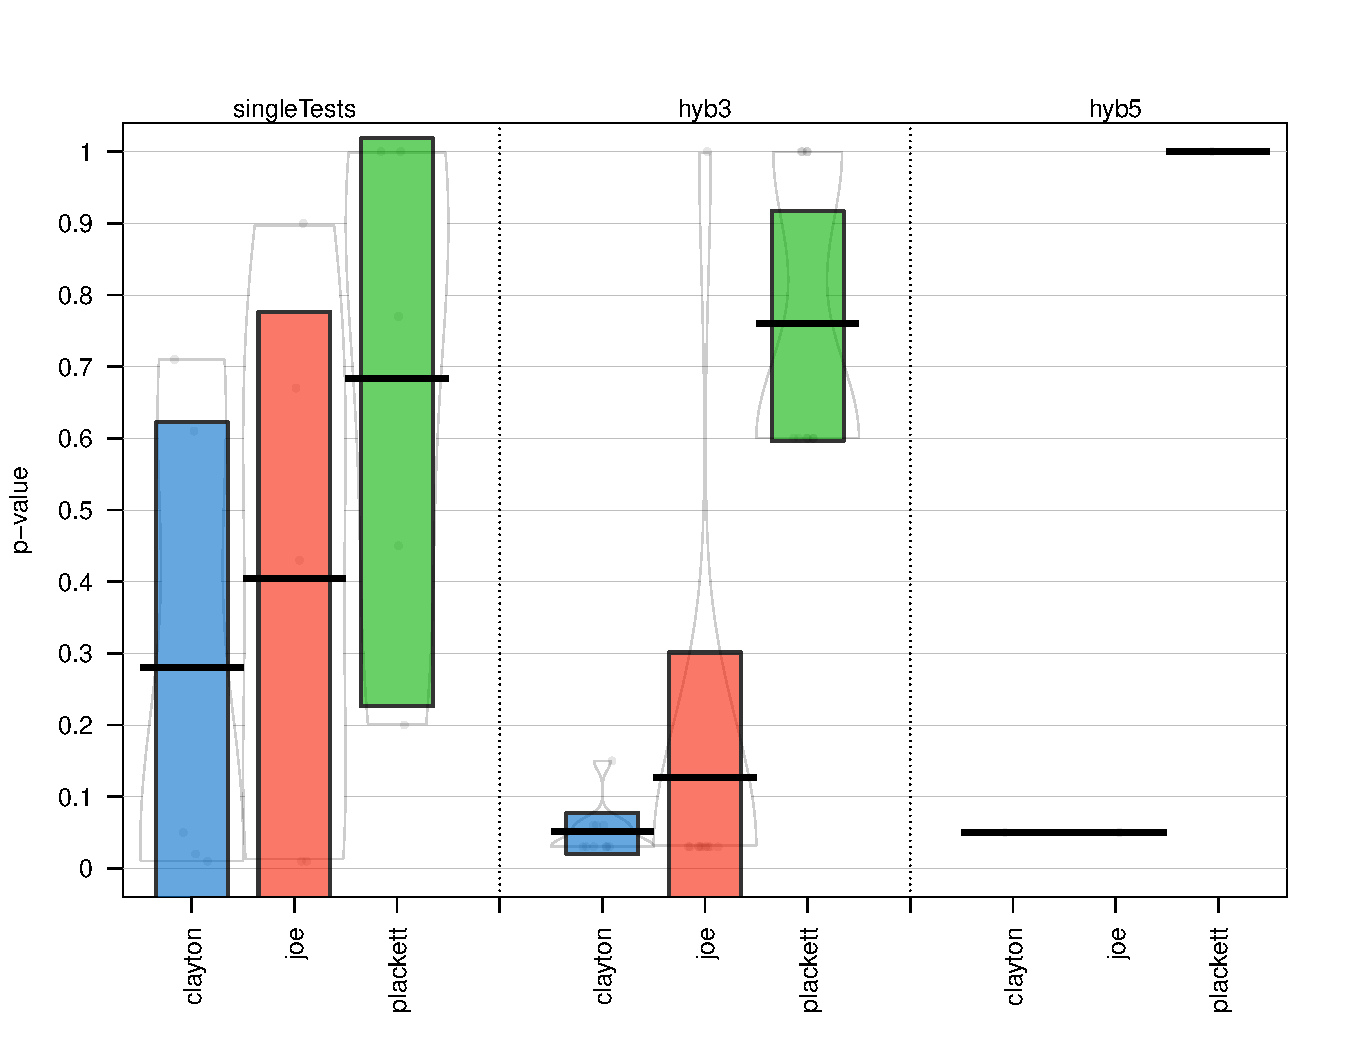
\includegraphics[width = 85mm]{img/Functionality_Pirateplot.pdf}
\caption{\mycolor Resulting $p$-values of different hybrid tests for the Clayton, Joe, and Plackett copula visualized in a pirateplot. \bk}
\label{Pirateplot_Example}
\end{figure}

\mycolor Specifying \code{hybrid = c(1, 3, 5)} means that the $p$-values of the single tests (column \code{singleTests} in Figure \ref{Pirateplot_Example}), the $p$-values of hybrid tests of size three (column \code{hyb3}), and size five (column \code{hyb5}) should be plotted, separated by selected copulae. For example, we focus on the column \code{hyb3} for the Plackett copula. It contains information of all hybrid tests, which include three single tests for the Plackett copula. In this case, we can see that the mean of these tests is approximately 0.76, as shown by the thick horizontal line. All test $p$-values are shown by light-grey points in the column, indicating the heterogeneity of the tests ranging from 0.6 to 1. Finally, the green bar around the mean line is a Bayesian highest density interval, which provides the user, together with the shown density estimate in the grey continuous lines, further information about the distribution of the $p$-values. For more details on the \code{pirateplot} and its customization options, we refer to \citet{phillips2017yarrr}.\bk

\subsection{Fire-and-forget}\label{subsec:fire_forget}
The R-package \pkg{gofCopula} includes all the discussed tests in Section \ref{sec:gof}. For each of the tests, a separate function is implemented with a variety of arguments. We give shortly the most important arguments all the tests share before we go into details about the structure of the package. 
\begin{itemize}
	\item \code{copula}: The copula to test for. \mycolor Possible options depend on the test and dimension. \bk
	\item \code{x}: A matrix containing the data with rows being observations and columns being variables.
	\item \code{M} (default: 1000): Number of bootstrapping loops.
	\item \code{param} (default: 0.5): The copula parameter to use if it shall not be estimated. In case of the Gumbel copula, the default value is set to 1.5.
	\item \code{param.est} (default: \code{TRUE}): Boolean. \code{TRUE} means that \code{param} will be estimated.
	\item \code{margins} (default: \code{ranks}): Specifies which estimation method shall be used. The default \code{ranks} stands for formula (\ref{eqn:npm}), which is the standard approach to convert data. Alternatively, the following distributions can be specified: \code{beta}, \code{cauchy}, Chi-squared (\code{chisq}), \code{f}, \code{gamma}, Log normal (\code{lnorm}), Normal (\code{norm}), \code{t}, \code{weibull}, Exponential (\code{exp}).
	\mycolor \item \code{flip} (default: 0): The parameter to rotate the copula by 90, 180, 270 degrees clockwise. Only applicable for bivariate copula. \bk
	\item \code{seed.active} (default: \code{NULL}): Sets the seeds for the bootstrapping procedure. It has to be either an integer or a vector of \code{M+1} integers. If an integer is provided, the seeds for the bootstrap samples will be simulated based on it. If \code{M+1} seeds are given, these are used in the bootstrapping procedure. In the default case (\code{seed.active = NULL}), R generates the seeds from the computer runtime.
	\item \code{processes} (default: 1): The number of parallel processes which are performed to speed up the bootstrapping. Should not be larger than the number of logical processors. 
\end{itemize}

The package is coded as a \textit{fire-and-forget} package. Each of the single tests just requires the input of a dataset \code{x} and a \code{copula} to test for. All the other function parameters have reasonable default values such that quick first results can be achieved easily. The calculation steps of each GoF test function are the following:
\begin{itemize}
    \item \textit{Estimation of margins}: At first, the function transforms the data nonparametrically or parametrically to $\mathcal{U}[0,1]$; see Section \ref{sec:estimation}. This transformation is performed automatically, and a console statement informs the user about the transformation.
    \item \textit{Estimation of copula}: Afterward, the parameters of the copula model are estimated, so a two-stage estimation is applied; see Section \ref{sec:estimation}. Since a full ML estimation is computationally demanding, canonical ML estimation or inference for margins is applied. In case the ML estimation fails, the package automatically changes to inversion of Kendall's tau (see Section \ref{sec:estimation}), which guarantees a result. The user is informed about that switch by a warning message. 
    \item \textit{Bootstrapping}: Following the estimation of the copula parameters, the bootstrapping procedure will be performed, and the empirical $p$-value will be derived according to the test statistics in Section \ref{sec:bootstrap_test_stat}. Since the bootstrapping procedure can require a long computational time, it can pay out to parallelize the bootstrapping via the argument \code{processes}. 
\end{itemize}

\subsection{Hybrid testing and further functionality}\label{subsec:further_func}
Besides \code{gof} and the single tests, the package \pkg{gofCopula} offers additional functionality for the user. Next to descriptions, illustrative examples are provided, assuming the following was called beforehand:
\begin{example}
R> library("gofCopula")
R> data("IndexReturns2D", package = "gofCopula")
R> (res <- gof(copula = "normal", x = IndexReturns2D, M = 10, seed.active = 1,
+              tests = c("gofPIOSRn", "gofCvM", "gofKernel")))
\end{example}
\mycolor \vspace{-0.15cm}
\begin{example}
The margins will be estimated as: ranks
normal copula
\end{example} 
\bk \vspace{-0.5cm}
\begin{example}
Test gofPIOSRn is running
Test gofCvM is running            
Test gofKernel is running                                                                       
-------------------------------------------------------------------------------
Parametric bootstrap goodness-of-fit test with hybrid test and normal copula

Parameters:
theta.1 = 0.834742824340301

Tests results:
                p.value test statistic
PIOSRn              0.5    -0.11032857
Sn                  1.0     0.01520542
Kernel              0.3     0.56012429
hybrid(1, 2)        1.0             NA
hybrid(1, 3)        0.6             NA
hybrid(2, 3)        0.6             NA
hybrid(1, 2, 3)     0.9             NA

Please use the functions gofGetHybrid() and gofOutputHybrid() for 
display of subsets of Hybrid tests. To access the results, please
obtain them from the structure of the gofCOP object.
\end{example}
\bigskip
The functions are:

\begin{itemize}
    \item \code{gofCustomTest}: This function \mycolor has \bk - next to the standard arguments listed in Section \ref{subsec:fire_forget} - the argument \code{customTest}, a character string referencing one customized test loaded in the workspace. 
    The function containing this test should have two arguments: \mycolor a matrix named \code{x} for the dataset and a character string named \code{copula} for the copula to test for. \bk The whole calculation process, including the estimation of the margins and the copula, the calculation of the test statistics, and the bootstrapping of the $p$-value, is performed for this customized test. The procedure is shown using the test statistics of the \code{gofCvM} test.
\begin{example}
R> Testfunc = function(x, copula) {
+     C.theo = pCopula(x, copula = copula)
+        C.n = F.n(x, X = x)
+        CnK = sum((C.n - C.theo)^2)
+     return(CnK)
+ }

R> gofCustomTest(copula = "normal", x = IndexReturns2D, M = 10,
+                customTest = "Testfunc", seed.active = 1)
\end{example}
\begin{example}
The margins will be estimated as: ranks
-------------------------------------------------------------------------------
Parametric bootstrap goodness-of-fit test with Testfunc test and normal copula

Parameters:
theta.1 = 0.834742824340301

Tests results:
           p.value test statistic
Testfunc         1     0.01520542
\end{example}
\bigskip
    \item \code{gofGetHybrid}: Allows calculating hybrid test $p$-values for given $p$-values from customized tests with an object of class \code{"gofCOP"} generated in the package. Through the combination of \code{gofCustomTest} and \code{gofGetHybrid}, the users are not limited to the implemented tests in the package and have the opportunity to include their own tests in the analysis. Note that the function \code{gofOutputHybrid} has slightly different but comparable functionality, which is the reason it is not separately shown.
\begin{example}
R> gofGetHybrid(result = res, nsets = 5, p_values = c("MyTest" = 0.7,
+               "AnotherTest" = 0.3))
\end{example}
\begin{example}
-------------------------------------------------------------------------------
Hybrid test p-values for given single tests.

Parameters:
theta.1 = 0.834742824340301

Tests results:
                      p.value
PIOSRn                    0.5
Sn                        1.0
Kernel                    0.3
MyTest                    0.7
AnotherTest               0.3
hybrid(1, 2, 3, 4, 5)     1.0
\end{example}
\bigskip
    \item \code{gofTest4Copula}:~Returns for a given copula and a given dimension the list of applicable implemented tests.
\begin{example}
R> gofTest4Copula("gumbel", d = 5)
\end{example} 
\mycolor
\begin{example}
 [1] "gofArchmChisq"      "gofArchmGamma"      "gofArchmSnB"       
 [4] "gofArchmSnC"        "gofCustomTest"      "gofCvM"            
 [7] "gofKendallCvM"      "gofKendallKS"       "gofKS"             
[10] "gofRosenblattChisq" "gofRosenblattGamma" "gofRosenblattSnB"  
[13] "gofRosenblattSnC" 
\end{example} 
\bk
\bigskip
    \item \code{gofCopula4Test}: Returns for a given test the list of applicable implemented copulae.
\begin{example}
R> gofCopula4Test("gofPIOSTn")
\end{example}
\mycolor 
\vspace{-0.15cm}
\begin{example}
 [1] "normal"   "t"        "clayton"  "gumbel"   "frank"    "joe"     
 [7] "amh"      "galambos" "fgm"      "plackett"
\end{example}
\bk \bigskip
\item \code{gofCheckTime}: Estimates the time necessary to compute a selected single or group of GoF tests for a given number of bootstrapping rounds. This function uses an underlying regression model, so the results may vary from reality and also from the progress bar predictions. See Section \ref{sec:TimeParallelization}.
\begin{example}
R> gofCheckTime("normal", x = IndexReturns2D, tests = "gofRosenblattSnC", 
+               M = 10000, seed.active = 1)
\end{example}
\mycolor
\vspace{-0.15cm}
\begin{example}
The margins will be estimated as: ranks
An estimate of the computational time is under derivation.
Depending on the tests chosen, dimensionality and complexity of the data, this 
might take a while.
The computation will take approximately 0 d, 0 h, 10 min and 7 sec.
\end{example}
\bk \bigskip
    \item \code{gofco}: In the case a copula is already estimated with the package \pkg{copula}, one can provide an object of class \code{"copula"} to this function, and the parameter estimates are taken from the respective object.
\begin{example}
R> copObject = normalCopula(param = 0.8)
R> gofco(copObject, x = IndexReturns2D, M = 10, seed.active = 1,
+        tests = c("gofPIOSRn", "gofKernel"))
\end{example}
\begin{example}
The margins will be estimated as: ranks
Test gofPIOSRn is running
Test gofKernel is running                                                
-------------------------------------------------------------------------------
Parametric bootstrap goodness-of-fit test with hybrid test and normal copula

Parameters:
theta.1 = 0.8

Tests results:
             p.value test statistic
PIOSRn           0.9    -0.03641543
Kernel           0.2     0.57115224
hybrid(1, 2)     0.4             NA

Please use the functions gofGetHybrid() and gofOutputHybrid() for 
display of subsets of Hybrid tests. To access the results, please 
obtain them from the structure of the gofCOP object.
\end{example}
\end{itemize}

\subsection{Computational time and parallelization}
\label{sec:TimeParallelization}
One of the main drivers of long computation times is the high number of bootstrapping loops to achieve an asymptotically reliable result. As mentioned in Section \ref{subsec:further_func}, the build-in function \code{gofCheckTime} allows estimating the necessary computation time for a given test, copula, dataset, and number of bootstrapping rounds. Since different machines may have highly varying computation times for tests, the function relies on a regression using the number of bootstrapping loops as the independent variable. To ensure that the linear model is a valid assumption, we investigated the case using the functions \mycolor \code{gofKendallKS} \bk and \code{gofKernel}; see Section \ref{subsec:Time_Validation} for the results.

Enabling parallelization of the bootstrapping is necessary for computationally demanding tests as \code{gofPIOSTn} where, e.g., the computation for a dataset of 500 observations and 1000 bootstrapping loops for the $t$-copula can take, depending on the engine, up to several hours. However, even for tests with faster computation time, parallelization is useful given the sample size and the number of bootstrapping loops is sufficiently high. This is shown in Table \ref{Time_Fast_Tests} in the form of a comparison between the computation times of five tests \mycolor for five copulas \bk without and with parallelization on four cores. The dataset contained \mycolor $n = 500$ \bk observations randomly generated from a bivariate standard normal distribution, and the number of bootstrapping loops was set to $M = 1000$.

\begin{table}[H]
\centering
\mycolor
\begin{tabular}{lrrrrr}
  \toprule
Test & normal & t & clayton & gumbel & frank \\ 
  \midrule
  \multicolumn{1}{l}{\textit{\#processes = 1:}}\\
  & & & & &\\
  gofKendallCvM & 200.33 & 530.22 & 166.85 & 249.86 & 167.81 \\ 
  gofKendallKS & 115.43 & 450.50 & 100.69 & 172.26 & 88.83 \\ 
  gofPIOSRn & 84.90 & 433.32 & 67.20 & 148.09 & 50.98 \\ 
  gofRosenblattChisq & 75.79 & 431.02 & 73.09 & 143.94 & 55.97 \\ 
  gofRosenblattGamma & 75.28 & 420.31 & 75.77 & 142.16 & 52.17 \\ 
   \midrule
  \multicolumn{1}{l}{\textit{\#processes = 4:}}\\
  & & & & &\\
  gofKendallCvM & 106.19 & 288.86 & 104.29 & 140.25 & 94.69 \\ 
  gofKendallKS & 68.73 & 238.55 & 56.13 & 89.02 & 53.00 \\ 
  gofPIOSRn & 48.81 & 235.35 & 47.37 & 83.71 & 33.66 \\ 
  gofRosenblattChisq & 49.43 & 230.33 & 45.83 & 85.70 & 35.47 \\ 
  gofRosenblattGamma & 47.45 & 234.50 & 48.41 & 82.04 & 37.32 \\  
   \bottomrule
\end{tabular} \bk
\caption{Computation times in seconds without and with parallelization using an Intel Core i7-4712MQ CPU with 2.3 GHz on a 64-Bit Windows 10 system.}
\label{Time_Fast_Tests}
\end{table}
\section{Simulations}
\label{sec:simulation_study}
\subsection{Empirical process of using the package}\label{sec:empirical_process_sim}
We would like to illustrate the power of the GoF tests with the use of the \pkg{gofCopula} package. In practice, one is often confronted with realizations of random variables for which an adequate copula model has to be found, as, e.g., in the two examples from the financial domain provided in Section \ref{sec:application}.
To illustrate the procedure, we focus in this Section on an easy replicable example. For this purpose, we start by simulating $n = 1000$ observations from a Clayton copula with Kendall's $\tau = 0.5$.
\mycolor
\begin{example}
R> library("gofCopula")
R> param = iTau(copula = claytonCopula(), tau = 0.5)
R> n = 1000; set.seed(1)
R> x = rCopula(n = n, copula = claytonCopula(param = param))
\end{example}
To gain a better understanding of the data, Figure \ref{Sim_Clayton_Plot_Sec_5} shows the simulated data with different margins, reflecting the typical shape of the Clayton copula.

\begin{example}
R> par(mfrow = c(1,2))
R> u = cbind(ecdf(x[,1])(x[,1]), ecdf(x[,2])(x[,2])) * n / (n + 1)
R> plot(u, col = "blue3", pch = 19, cex.lab = 1.25, 
+       xlab = expression(u[1]), ylab = expression(u[2]))
R> plot(qnorm(u), col = "blue3", pch = 19, cex.lab = 1.25,
+       xlab = expression(x[1]), ylab = expression(x[2]))
R> par(mfrow = c(1,1))
\end{example}
\vspace{-0.7cm}
\begin{figure}[H]
	\centering
 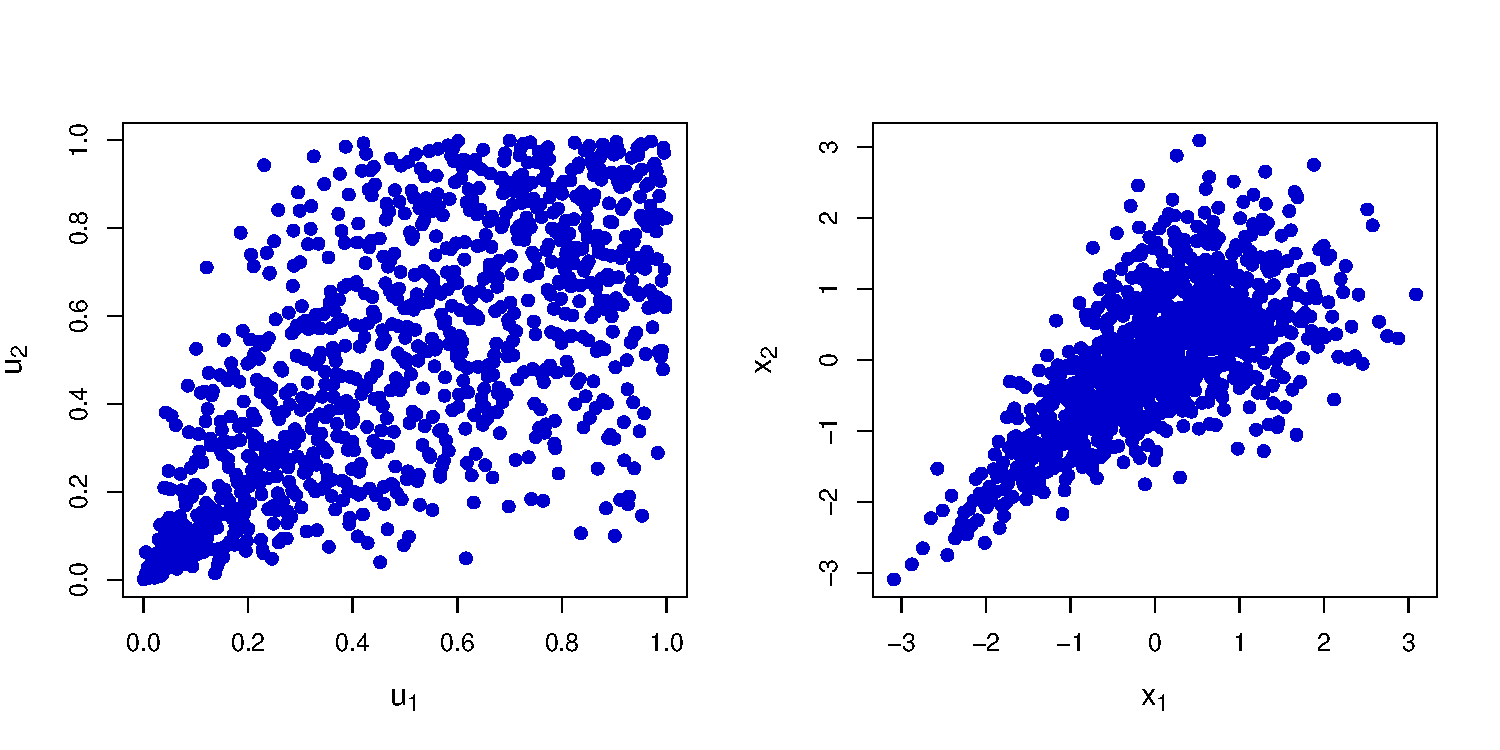
\includegraphics[width=110mm]{img/Simulated_Example.pdf}
	\caption{$n = 1000$ observations sampled from a Clayton copula with $\tau = 0.5$. \mycolor Margins are transformed using ranks on the left plot and are standard normal on the right plot. \bk}
	\label{Sim_Clayton_Plot_Sec_5}
\end{figure}

\mycolor To make an adequate decision on which copula should be used in the respective modeling task, the GoF testing should involve more than looking at one or two test results and should consider a reasonable amount of potential copula models. We structure our procedure by testing for three groups of copulae separately: Elliptical, Archimedean, and extreme value (EV) copulae. In the function call, we select the FGM and Plackett copulae together with the EV category, although they do not belong to any of the three categories. Elliptical copulae include the normal and $t$-copula, while the Clayton, Gumbel, Frank, Joe, and AMH copulae are the Archimedean ones. Galambos, Husler-Reiss, Tawn, and $t$-EV belong to the EV category. Notice that this categorization could be modified, as, e.g., the Gumbel copula is also an EV copula. However, the given approach offers not only a logical structuring of the modeling task, but leads to using a close to maximal number of tests via only three function calls. The bootstrap parameters were set to $M = 100$ and $MJ = 1000$. As this task is computationally demanding, we set the argument \code{processes = 7} to speed up the calculation using parallelization on 7 cores. We use the default \code{margins = "ranks"} and set \code{seed.active = 10} for reproducibility.
\begin{example}
R> cop_1 = gof(x = x, M = 100, MJ = 1000, processes = 7, seed.active = 10, 
+              copula = c("normal", "t"))
R> cop_2 = gof(x = x, M = 100, MJ = 1000, processes = 7, seed.active = 10, 
+              copula = c("clayton", "gumbel", "frank", "joe", "amh"))
R> cop_3 = gof(x = x, M = 100, MJ = 1000, processes = 7, seed.active = 10, 
+              copula = c("galambos", "huslerReiss", "tawn", "tev", "fgm", "plackett"))
\end{example}

\bk To evaluate the gained \mycolor objects \bk of class \code{"gofCOP"}, one can manually inspect the resulting $p$-values and look closer at the performances and differences between the single tests and the corresponding hybrids. However, the easiest and most informative way is to visualize the $p$-values, which is done using the \code{plot} function.
\mycolor
\begin{example}
R> plot(cop_1)
\end{example}
\vspace{-1cm}
\begin{figure}[H]
	\centering
 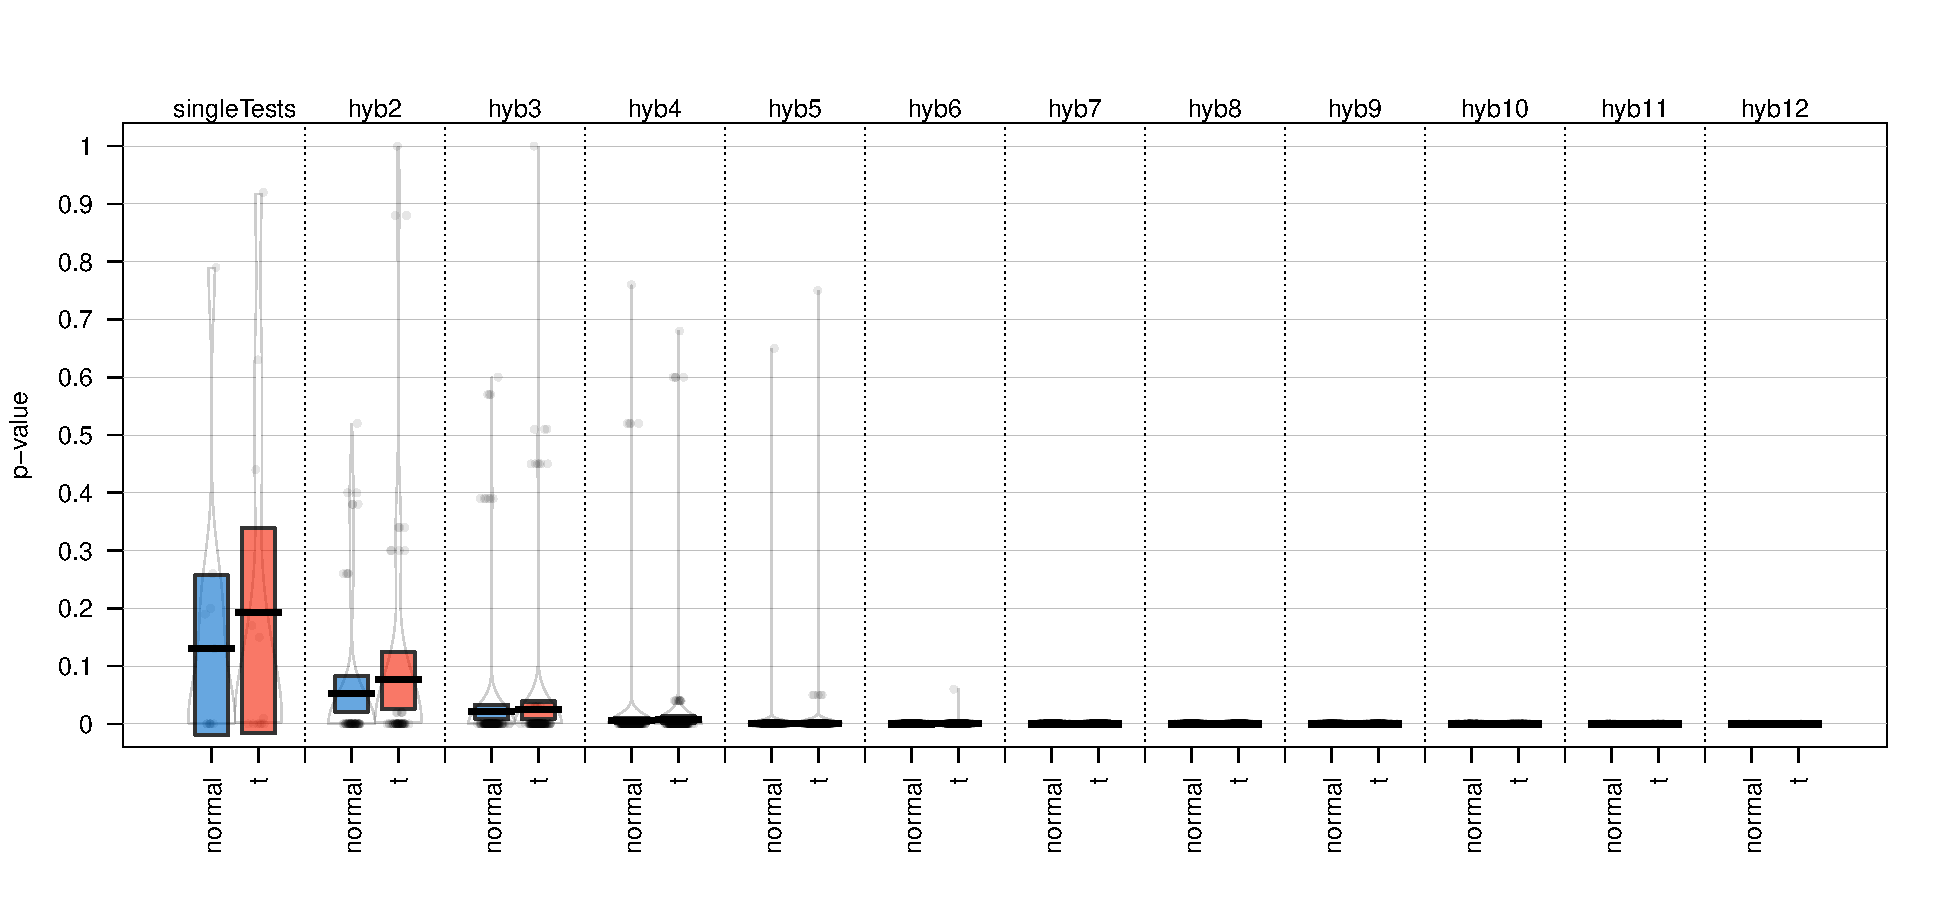
\includegraphics[width=\textwidth]{img/Simulation_cop1.pdf}
	\caption{\mycolor $p$-values of the hybrid tests for the data from Figure \ref{Sim_Clayton_Plot_Sec_5} for elliptical copulae.}
	\label{fig:Sim_cop1}
\end{figure}

\begin{example}
R> plot(cop_2)
\end{example}
\vspace{-1cm}
\begin{figure}[H]
	\centering
 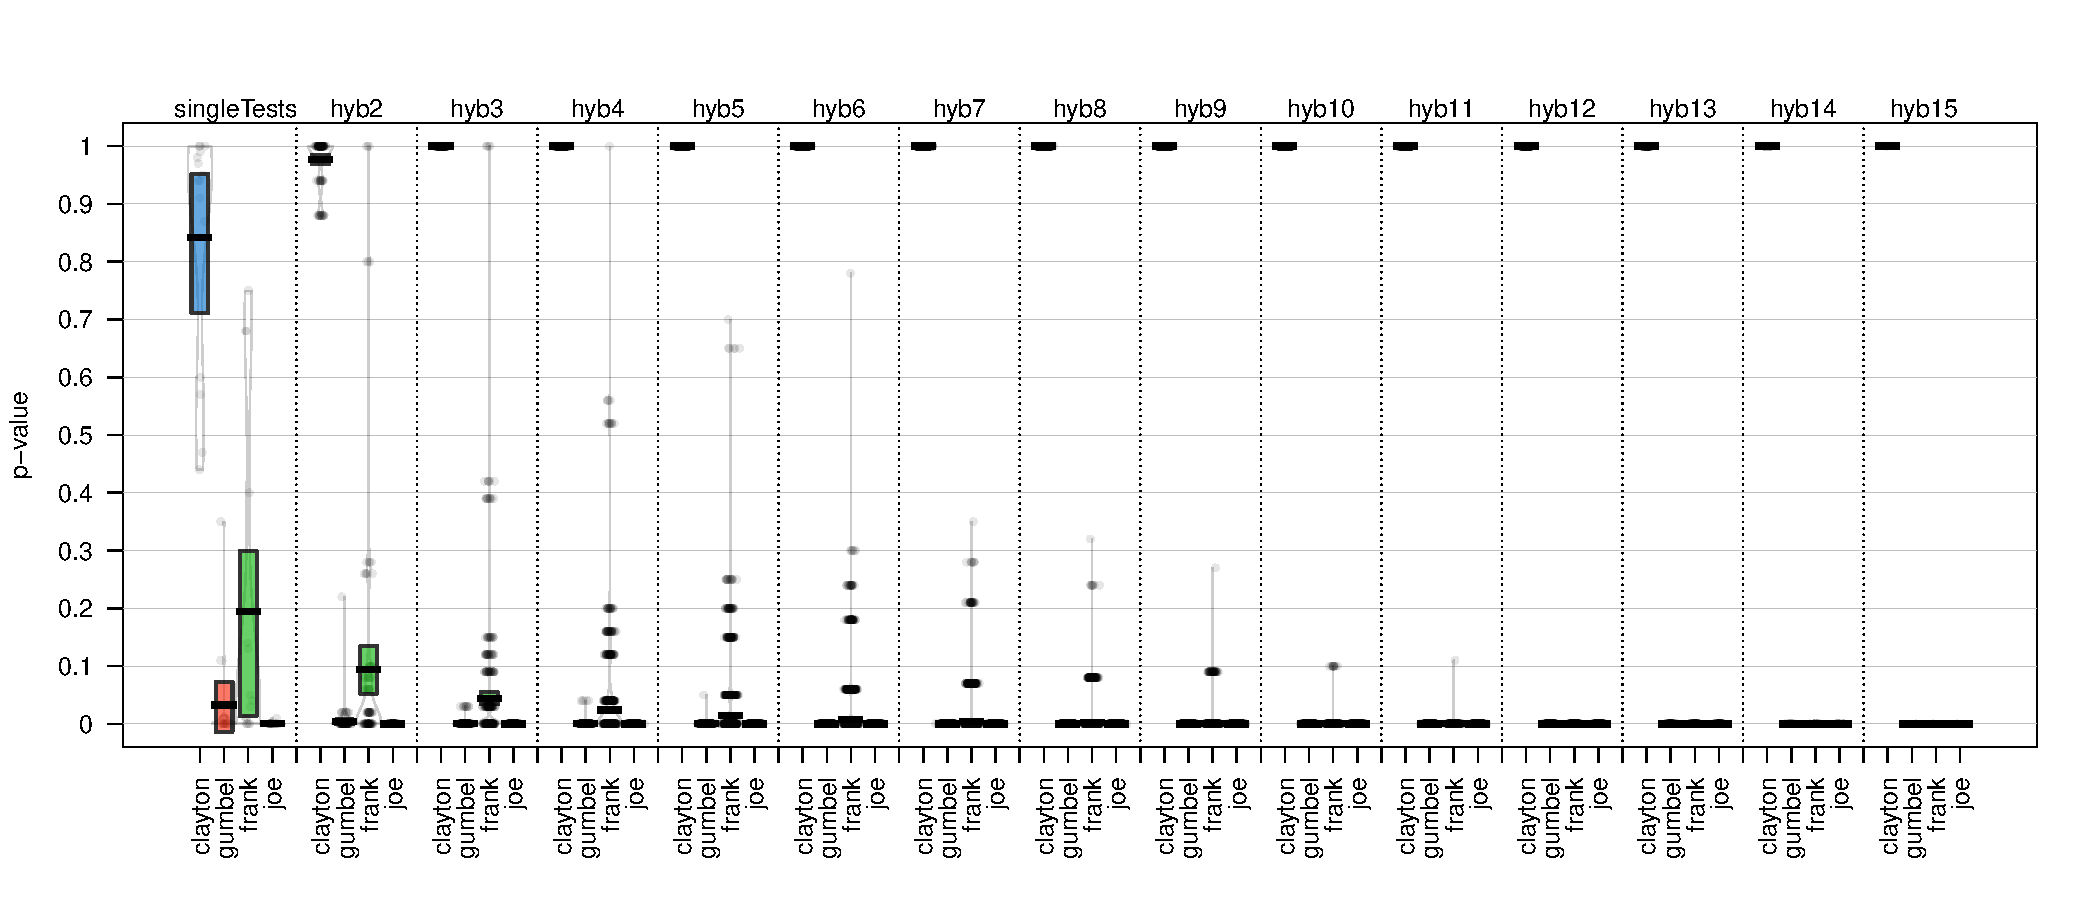
\includegraphics[width=\textwidth]{img/Simulation_cop2.pdf}
	\caption{\mycolor $p$-values of the hybrid tests for the data from Figure \ref{Sim_Clayton_Plot_Sec_5} for Archimedean copulae.}
	\label{fig:Sim_cop2}
\end{figure}

\begin{example}
R> plot(cop_3)
\end{example}
\vspace{-1cm}
\begin{figure}[H]
	\centering
 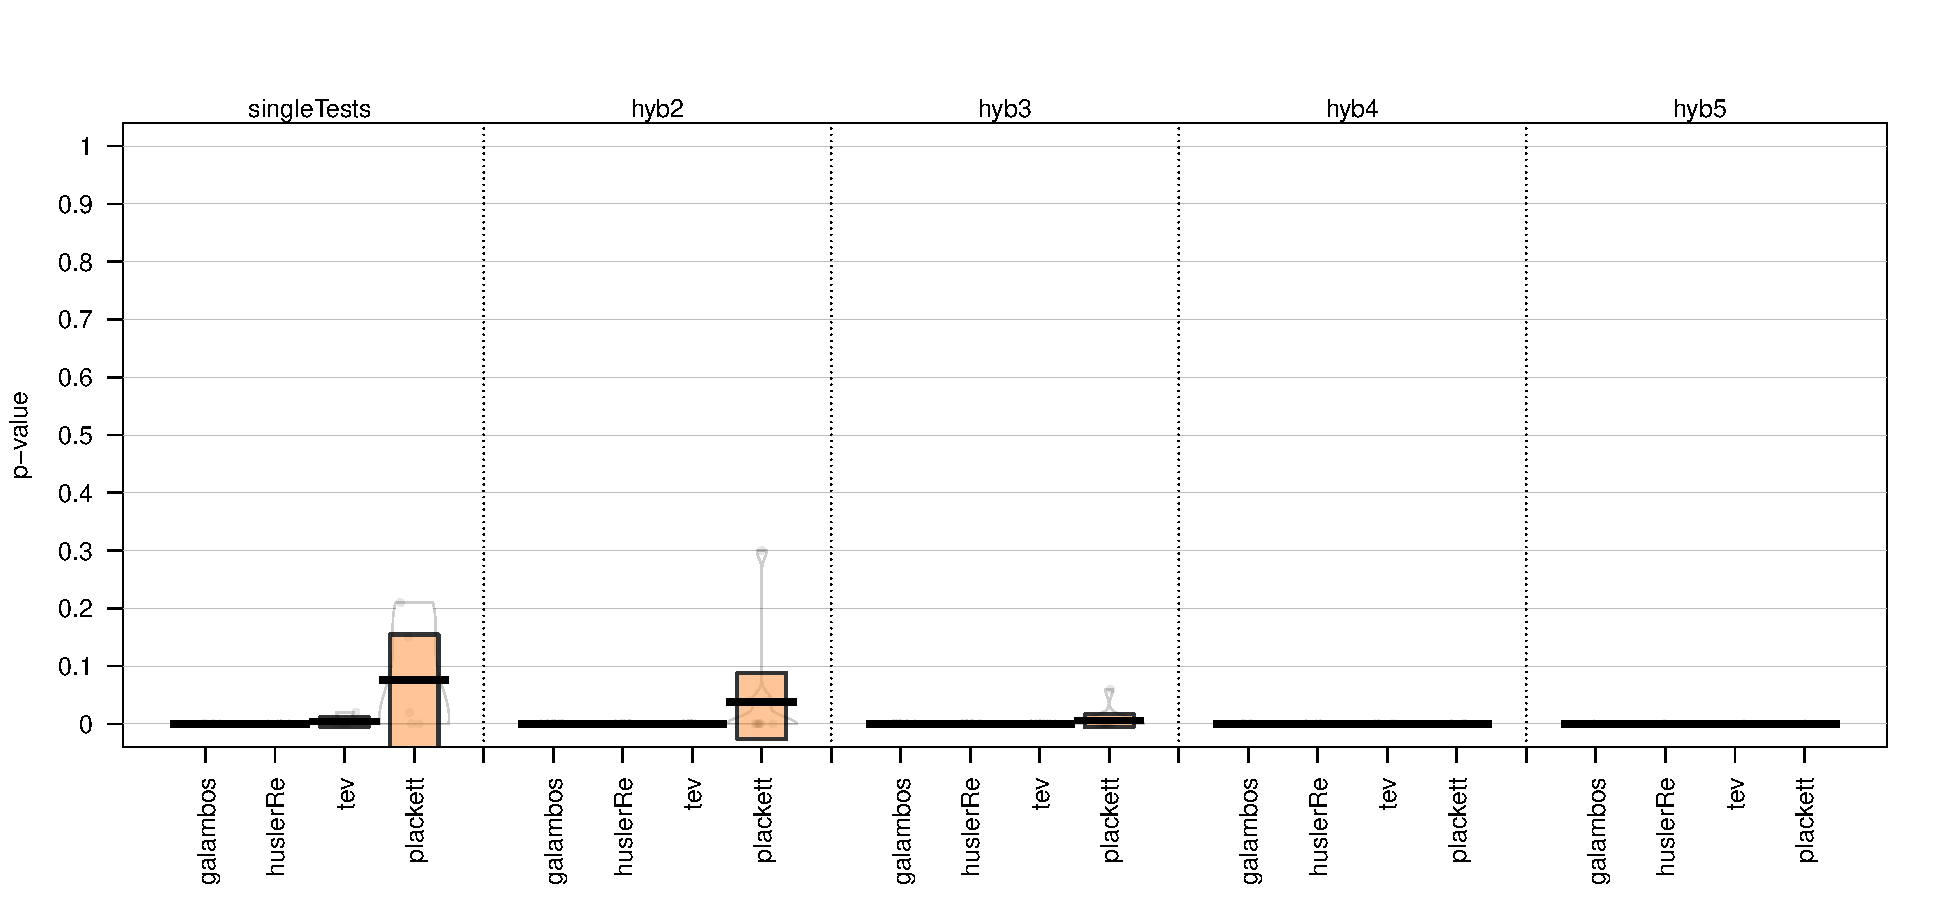
\includegraphics[width=\textwidth]{img/Simulation_cop3.pdf}
	\caption{\mycolor $p$-values of the hybrid tests for the data from Figure \ref{Sim_Clayton_Plot_Sec_5} for EV, FGM, and Plackett copulae.}
	\label{fig:Sim_cop3}
\end{figure}
Interpreting Figures \ref{fig:Sim_cop1}, \ref{fig:Sim_cop2}, and \ref{fig:Sim_cop3} clearly shows the ability of the tests to detect the true copula. The column \code{singleTests} in Figure \ref{fig:Sim_cop2} indicates that the Clayton copula is appropriate. The decision is supported by the higher-order hybrid tests, as all $p$-values except for the Clayton copula become 0, strongly rejecting the $H_0$-hypothesis in these cases. Notice that similar to the introductory example in Section \ref{sec:PackageFuncs}, the AMG, Tawn, and FGM are automatically excluded, which is why they do not appear in the plots. Having such a result at hand, the user can proceed with the modeling task with the selected copula.
\bk
\subsection{Validating the model for the time estimation}\label{subsec:Time_Validation}
In the next step, we validate the assumption of using a linear model for estimating the computation time in \code{gofCheckTime}. \mycolor We have chosen the \code{gofKendallKS} test as a representative for the group of single bootstrapping tests and \code{gofKernel}, as the test having a double bootstrapping procedure. Both tests are available for all copulae in the bivariate case. For \code{gofKendallKS}, we measured the computation times for 12 copulae, varying numbers of bootstrap loops ($M$) and sample sizes ($n$) of the underlying dataset, which is simulated from a normal copula with Kendall's $\tau = 0.1$. This value is selected because it falls within the attainable interval of Kendall's $\tau$ for all copulae, see Table \ref{tbl:copula_characteristics}. For \code{gofKernel}, we fixed $n = 100$ and investigated the situation for 12 copulae, different $M$, and different sample sizes $MJ$ of the internal bootstrap. The results are shown in Figures \ref{fig:Time_KendallKS}, \ref{fig:Time_Kernel_1}, and \ref{fig:Time_Kernel_2}. The $t$-EV copula is not included in these illustrations due to its tremendous computation time, which can exceed the one of the $t$-Copula even for small sample sizes by a factor of 10 and higher. However, similar properties in the behavior of the computation time depending on the number of bootstrapping loops can be found. All calculations were performed without parallelization using an Intel Core i7-4712MQ CPU with 2.3 GHz on a 64-Bit Windows 10 system.

\mycolor For the \code{gofKendallKS} test, the computation time increases linearly with the number of bootstrapping loops $M$, while the $t$-Copula is generally the most time-demanding of the considered copulae. \bk This holds for all the analyzed sample sizes. A similar observation can be made for the \code{gofKernel} test. Here, a rapid increase in computation time is expected if both $M$ and $MJ$ increase. However, following \mycolor Figures \ref{fig:Time_Kernel_1} and \ref{fig:Time_Kernel_2}, \bk this is not the case, and a linear dependency is justifiable. Therefore, the package implements for \code{gofKernel} a linear model with $M$ and $MJ$ being independent variables.
\begin{figure}[H]
    \centering
 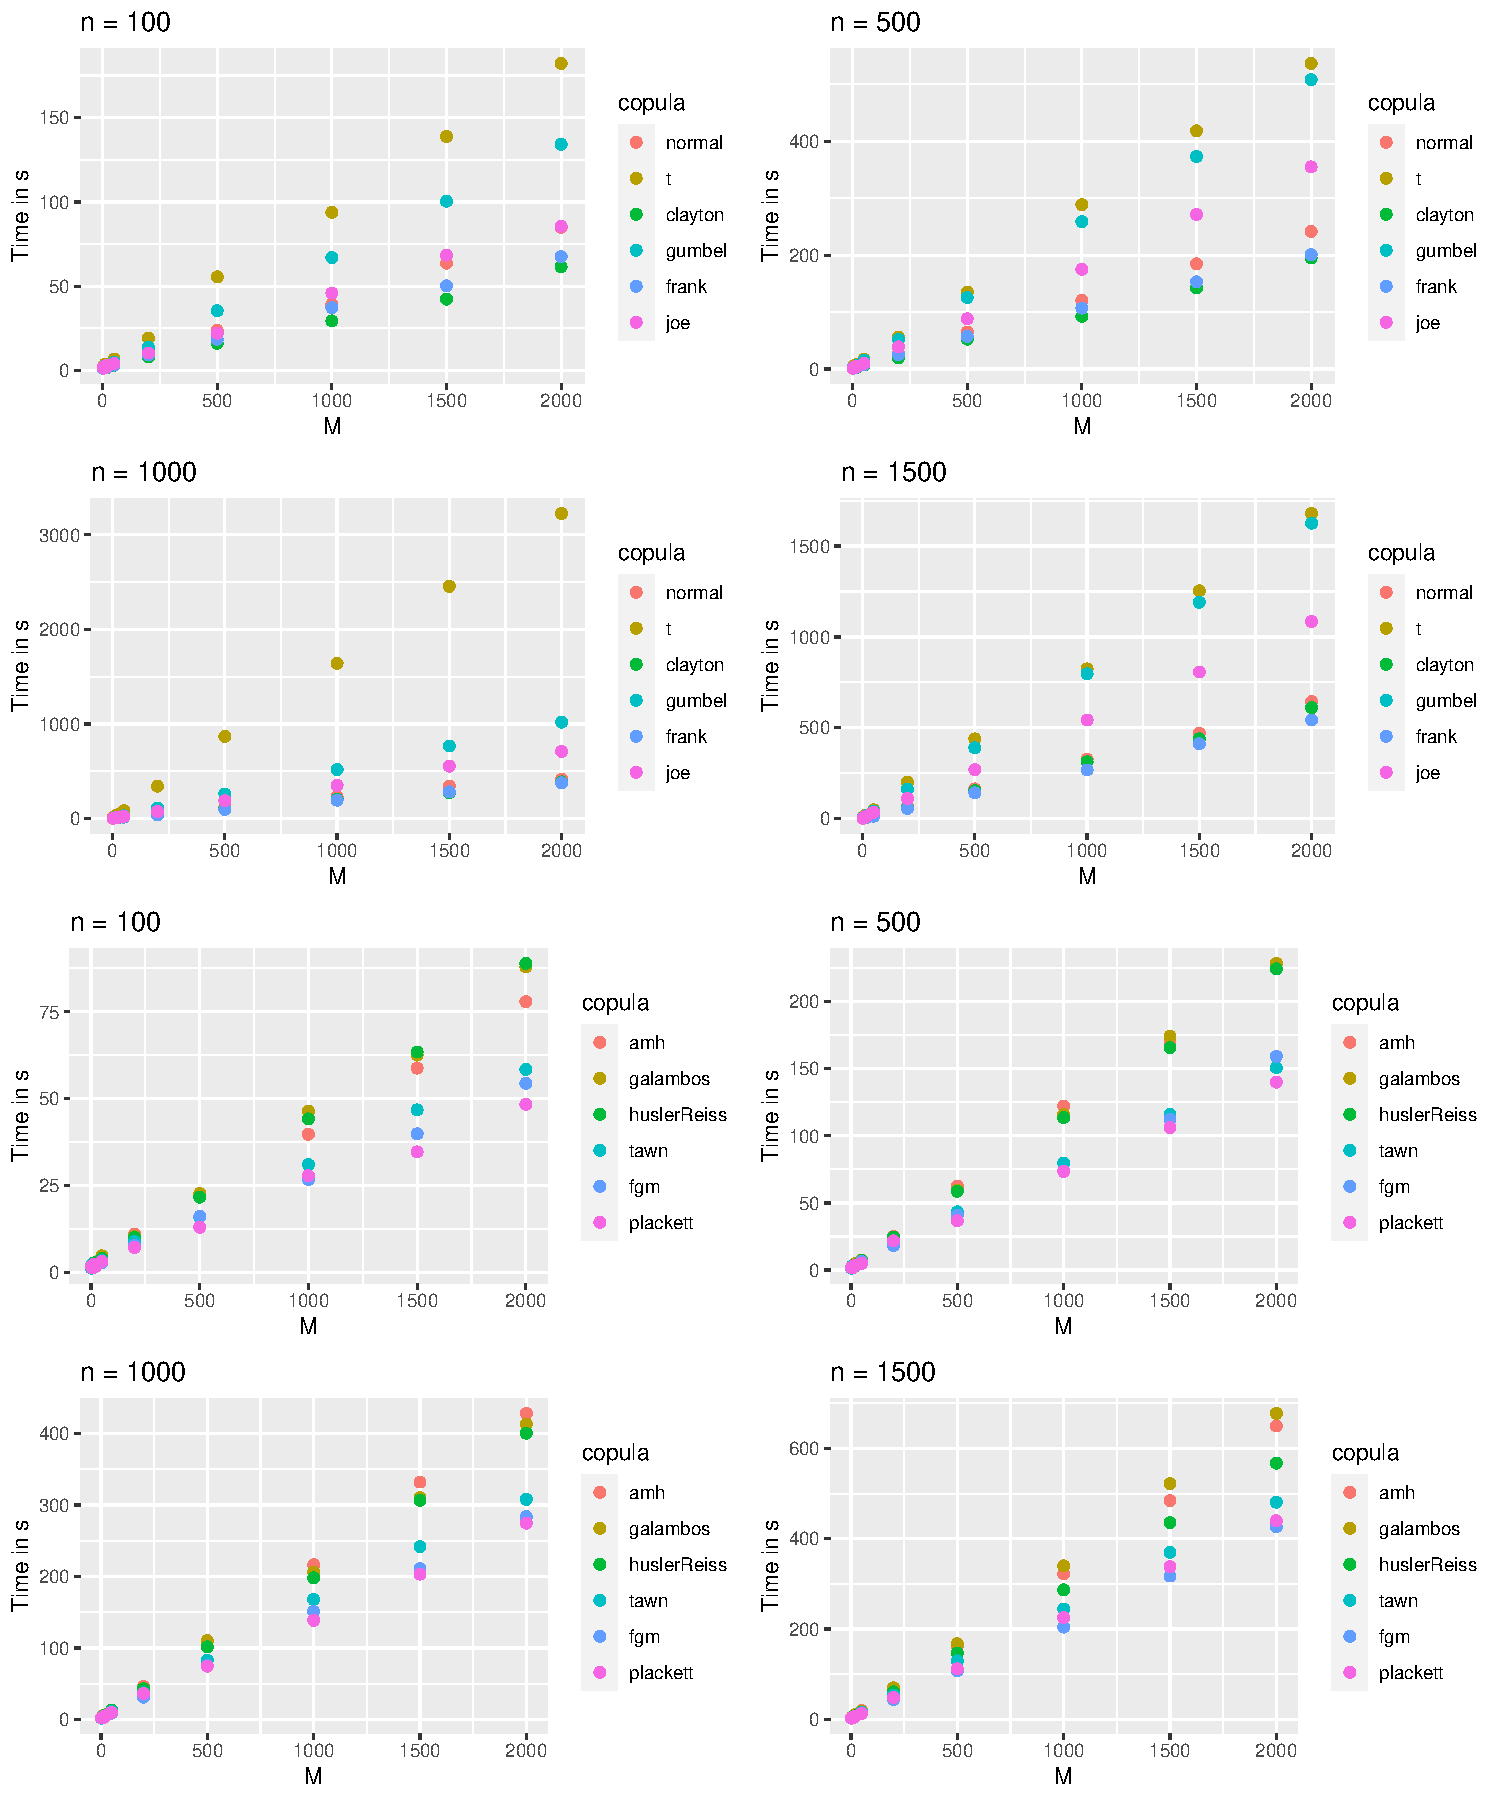
\includegraphics[width=\textwidth]{img/Time_KendallKS.pdf}
	\caption{Computation times of \mycolor \protect\code{gofKendallKS} \bk for different copulae, sample sizes $n$, and number of bootstrapping loops $M$.}
	\label{fig:Time_KendallKS}
\end{figure}

\begin{figure}[H]
	\centering
 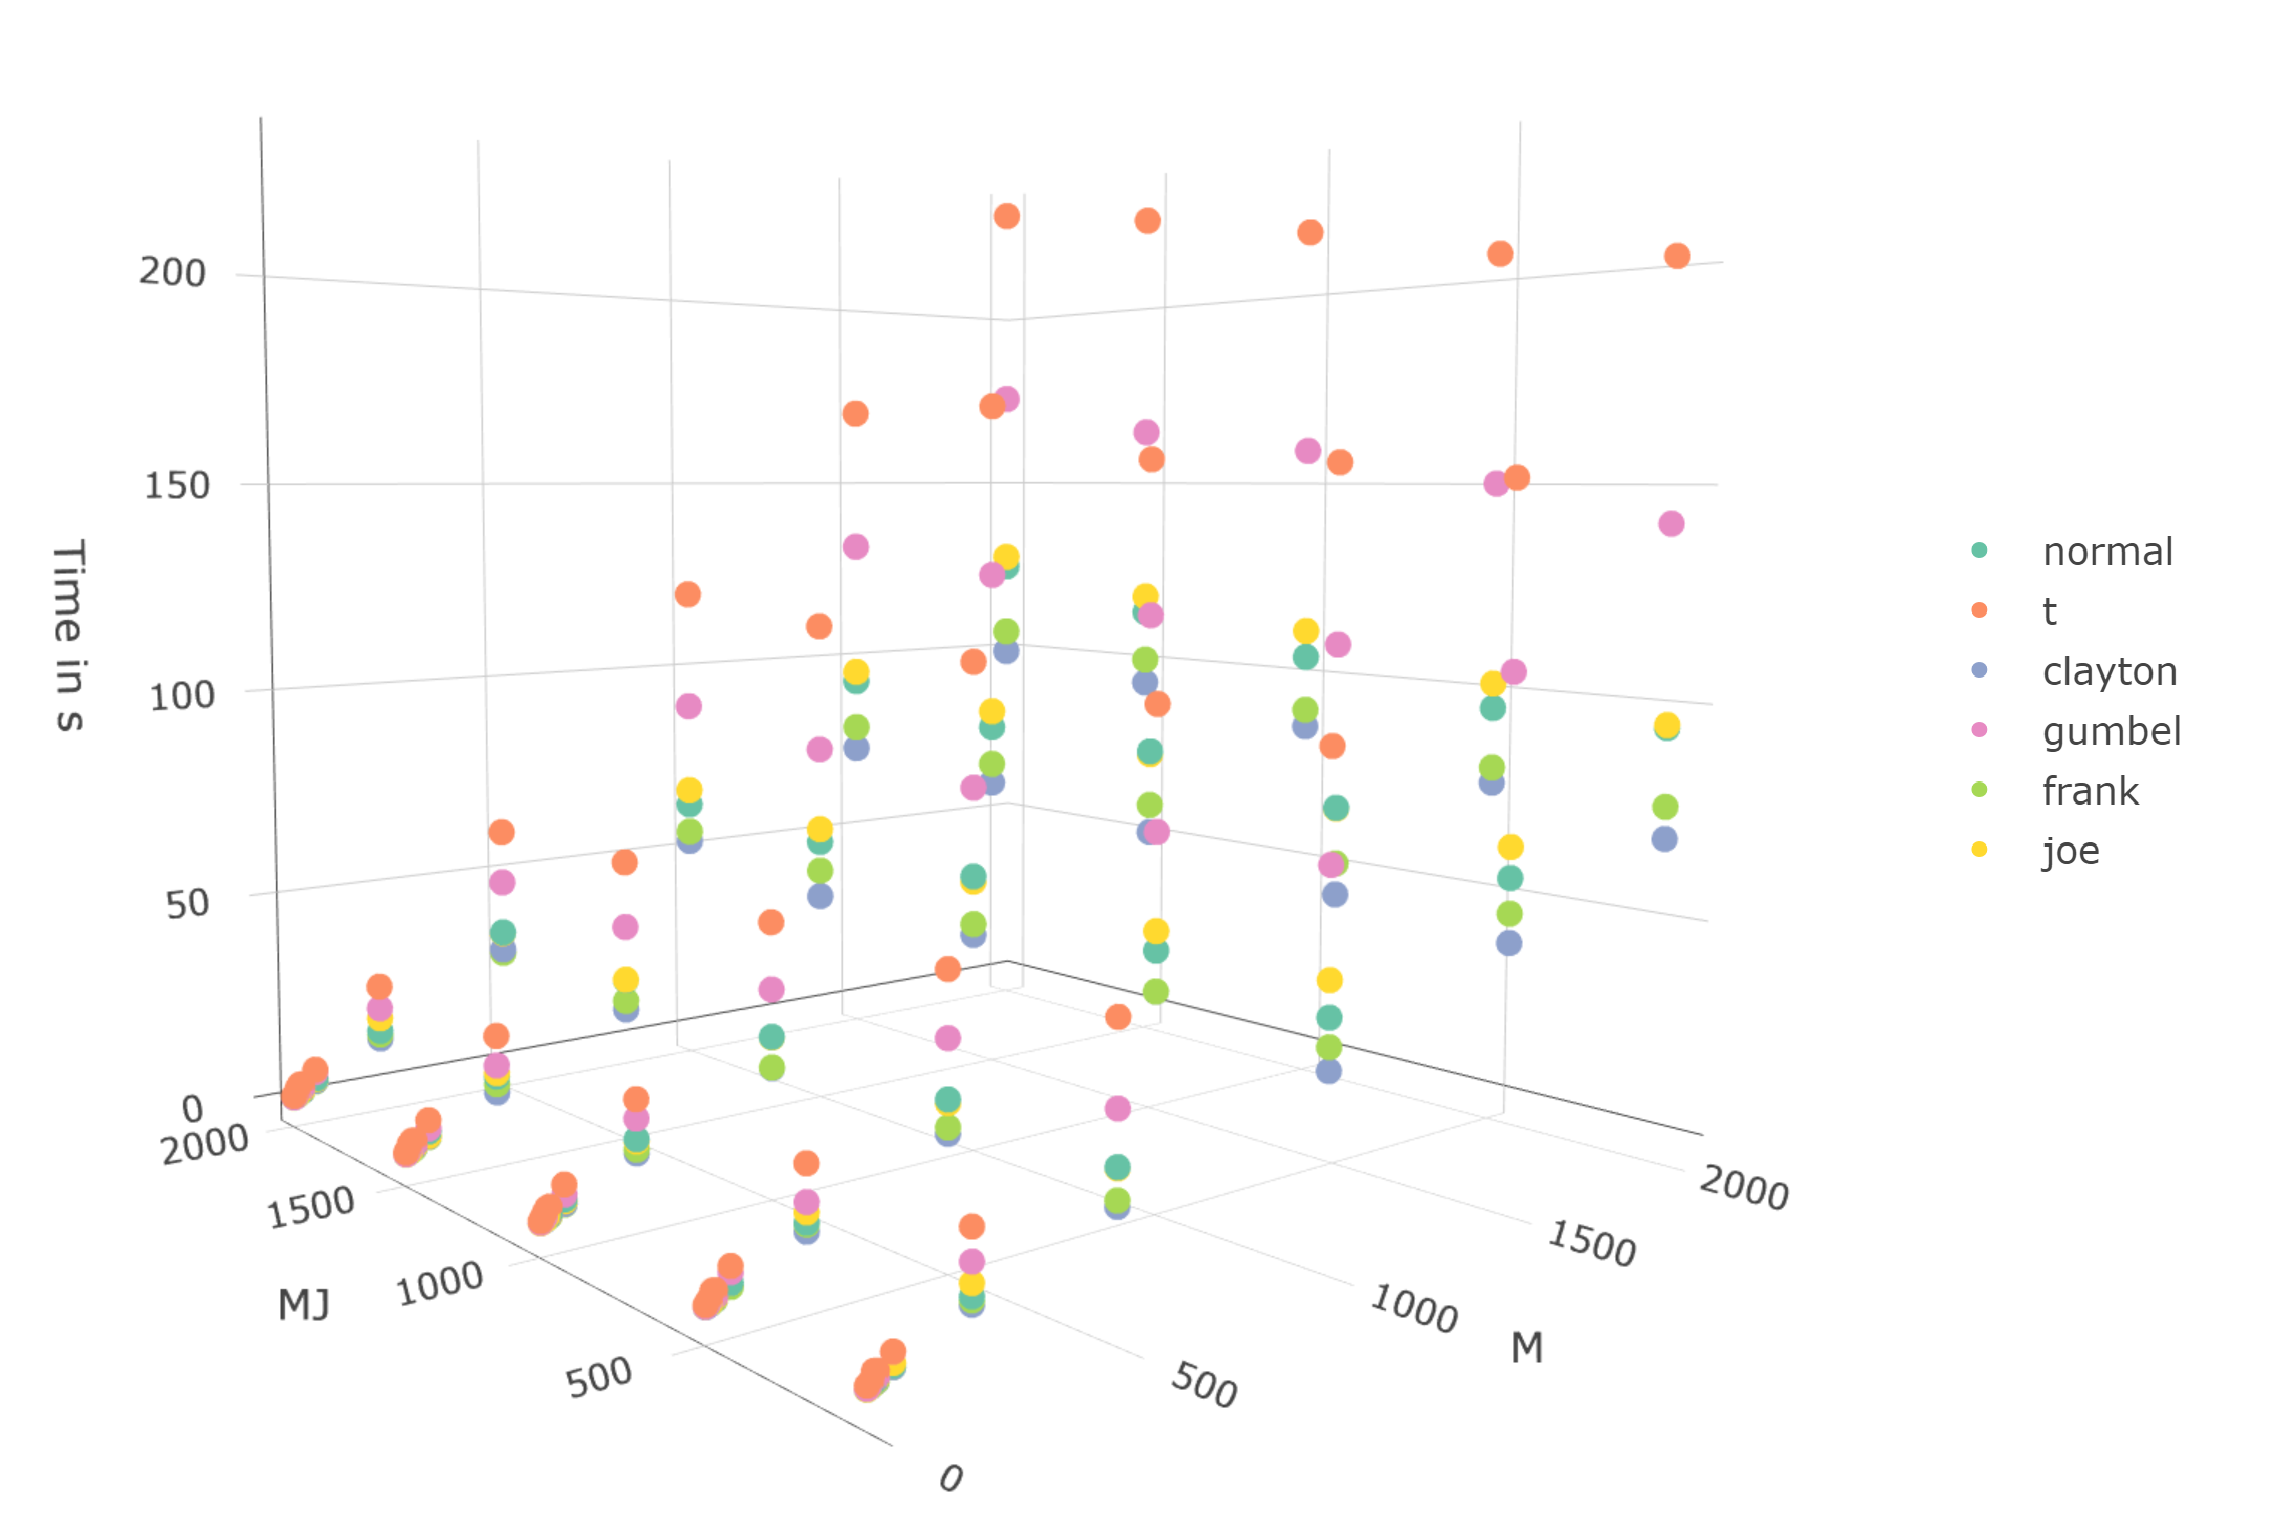
\includegraphics[width=11cm]{img/Time_Kernel_1.PNG}
	\caption{Computation times of \protect\code{gofKernel} for different copulae, number of bootstrapping loops $M$, and internal bootstrap sample size $MJ$.}
	\label{fig:Time_Kernel_1}
\end{figure}

\begin{figure}[H]
	\centering
 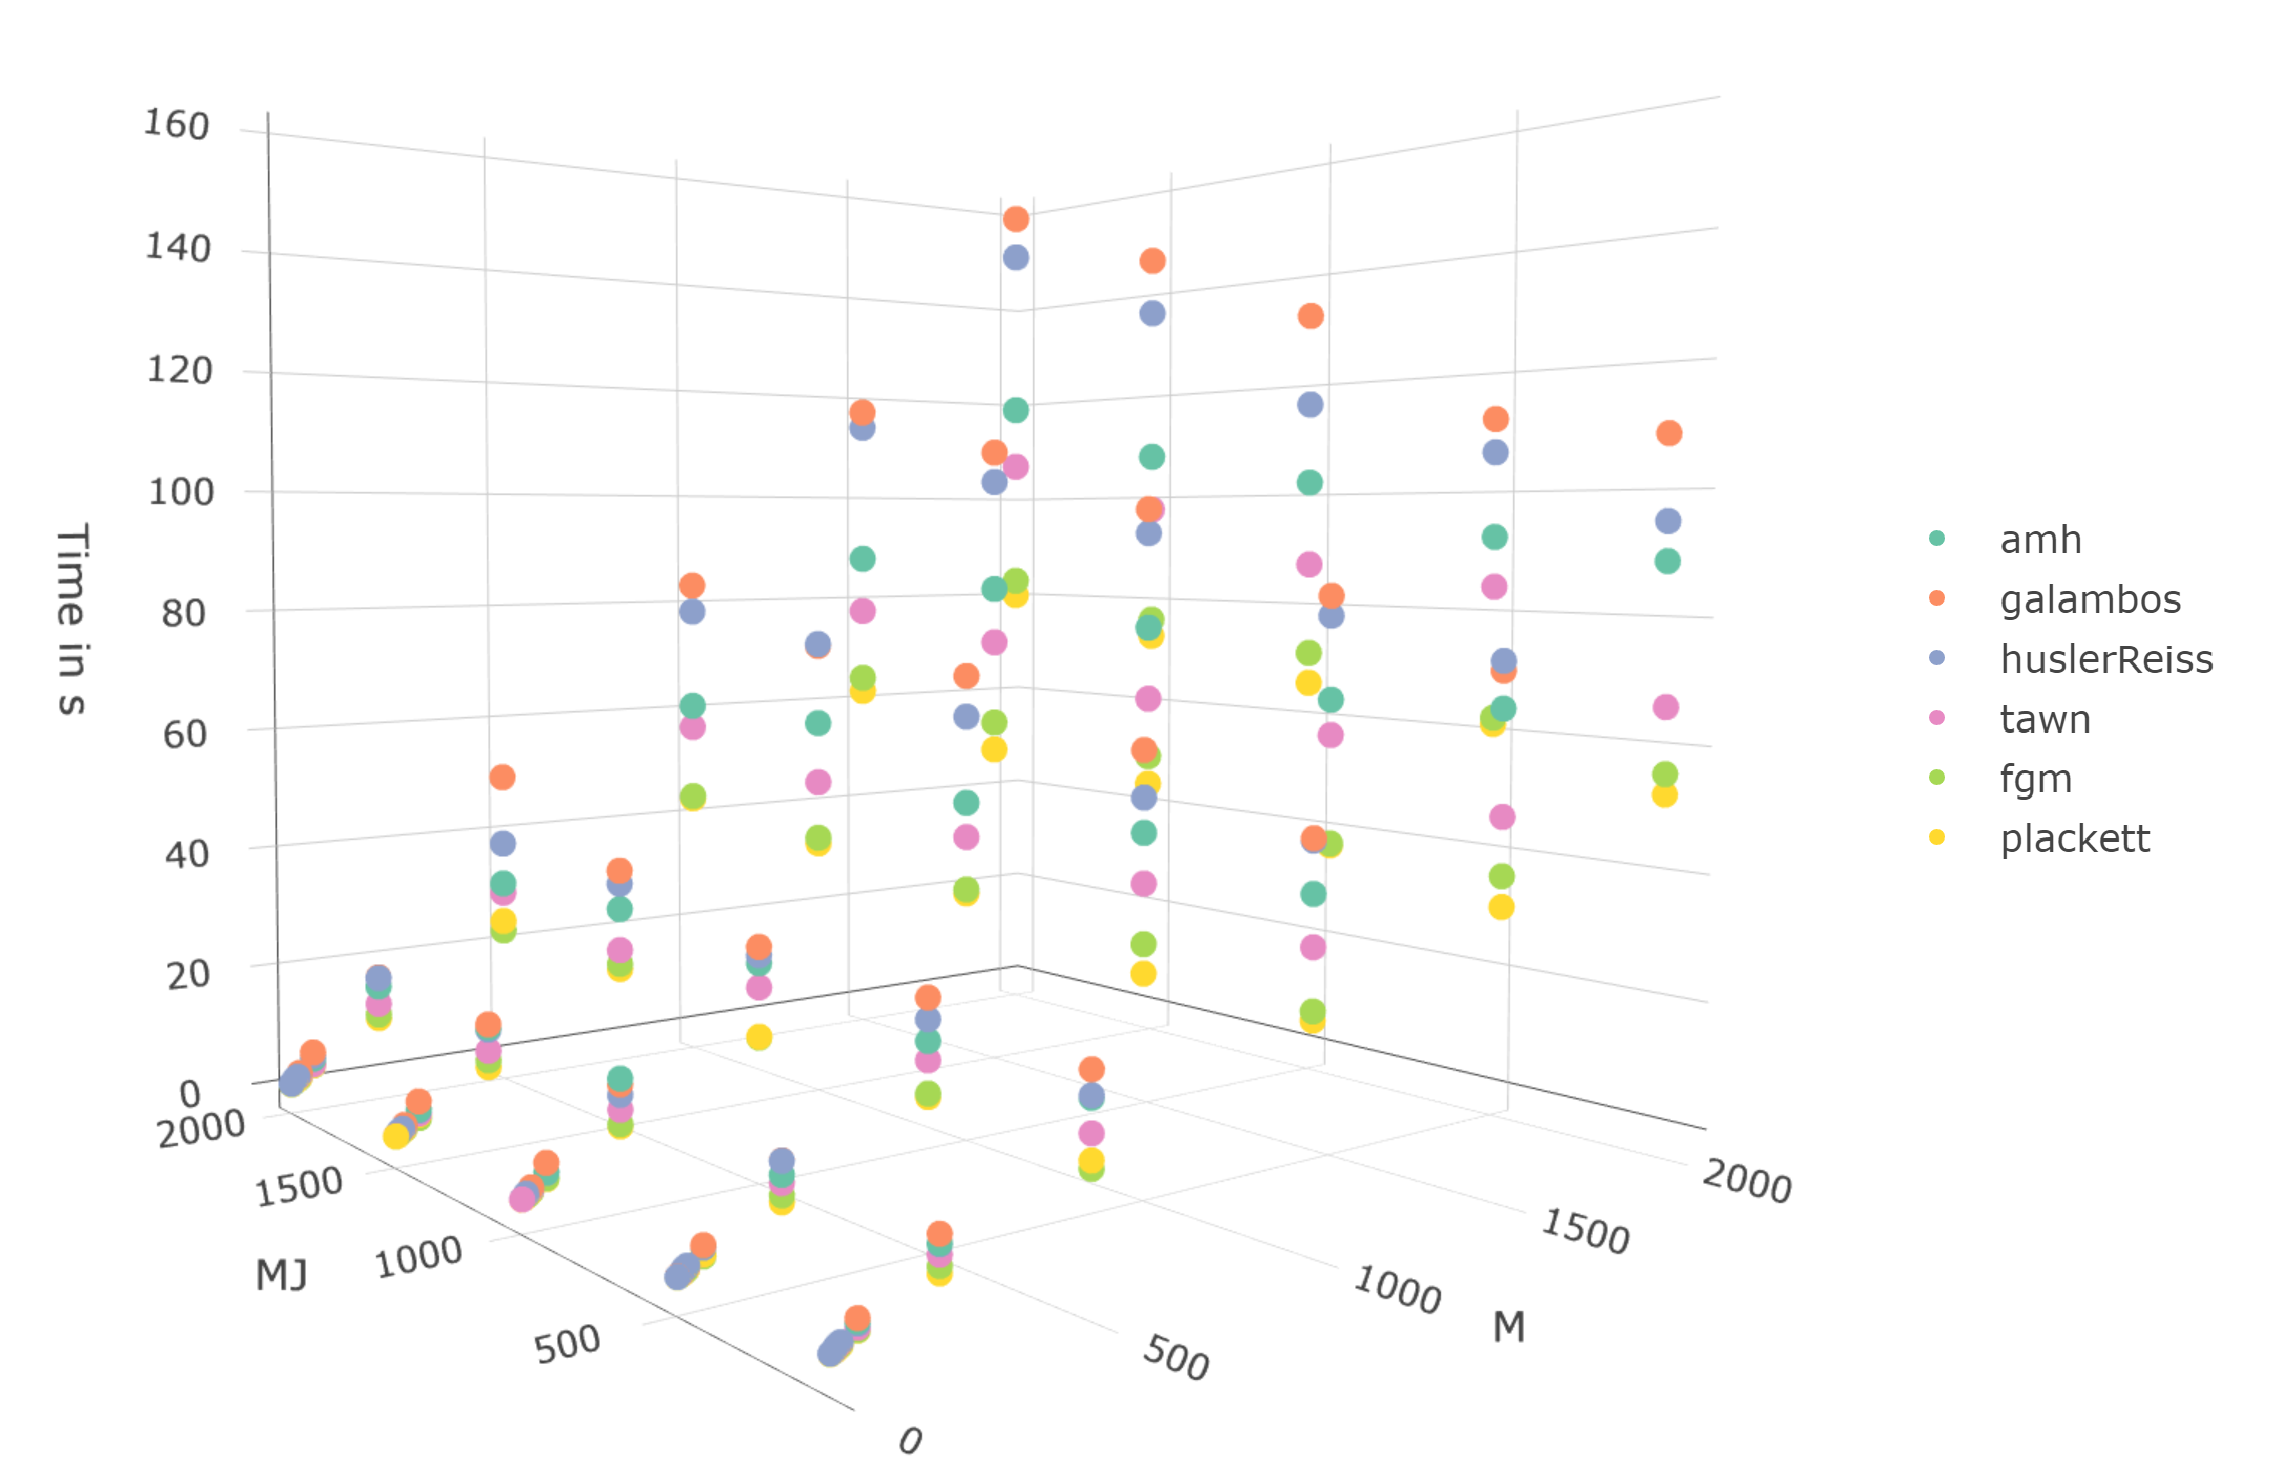
\includegraphics[width=11cm]{img/Time_Kernel_2.PNG}
	\caption{Computation times of \protect\code{gofKernel} for different copulae, number of bootstrapping loops $M$, and internal bootstrap sample size $MJ$.}
	\label{fig:Time_Kernel_2}
\end{figure}

\section{Application}
\label{sec:application}
\subsection{Cryptocurrency market}
\label{subsec:Cryptos}
We intend to demonstrate the functionality of the \pkg{gofCopula} package and show the empirical procedure as described in Section \ref{sec:empirical_process_sim} on a real-world example from the market of cryptocurrencies. To account for the relevant steps in a realistic application study, we split the procedure into \emph{Data Investigation} and \emph{Goodness-of-Fit testing}.

\subsubsection{Data investigation}
We have chosen Bitcoin (BTC) and Litecoin (LTC) for our analysis. The objective is to detect which copula is appropriate to model the dependence structure between BTC-LTC and check whether the copula changes over the years. For that purpose, we use the volatility-adjusted log-returns of the currencies in the time span from 2015 to 2018. The volatility correction was performed by fitting a GARCH(1,1) process to each time series for each year separately in order to extract their standardized residuals. These are included in the package as \code{CryptoCurrencies}, whereas each element of the list contains the data for a particular year. In order to gain a visual impression beforehand, we plotted the data with margins transformed to standard normal, leading to Figure \ref{Residual_BTC_LTC}. A strong dependency between both cryptocurrencies is visible, especially in the year 2018. Based on these residual diagrams, it is possible to take a guess which copula is the most adequate for the given situation. For 2015, one could possibly argue that the elliptical shape of a normal copula is present, while in 2016 and 2018, the shapes are more similar to the one of a $t$-Copula. Finally, for the year 2017, Figure \ref{Residual_BTC_LTC} shows a comparable plot to Figure \ref{Sim_Clayton_Plot_Sec_5} from the simulated example in Section \ref{sec:empirical_process_sim}, indicating a Clayton copula might be present. However, these visual impressions are to a certain degree subjective and need to be backed up by the GoF tests. Ideally, the test results would match our plot-based guesses.
\mycolor
\begin{example}
R> library("gofCopula")
R> data("CryptoCurrencies", package = "gofCopula")
R> par(mfrow = c(2,2))
R> years = as.character(2015:2018)

R> for(i in years){
+     x1 = CryptoCurrencies[[i]][,1]
+     x2 = CryptoCurrencies[[i]][,2]
+      n = length(x1)
+     plot(qnorm(cbind(ecdf(x1)(x1), ecdf(x2)(x2)) * n / (n + 1)), col = "blue3",
+          pch = 19, cex.lab = 1.25, main = i, xlab = "Bitcoin", ylab = "Litecoin")
+  }
R> par(mfrow = c(1,1))
\end{example}
\bk
\begin{figure}[H]
	\centering
 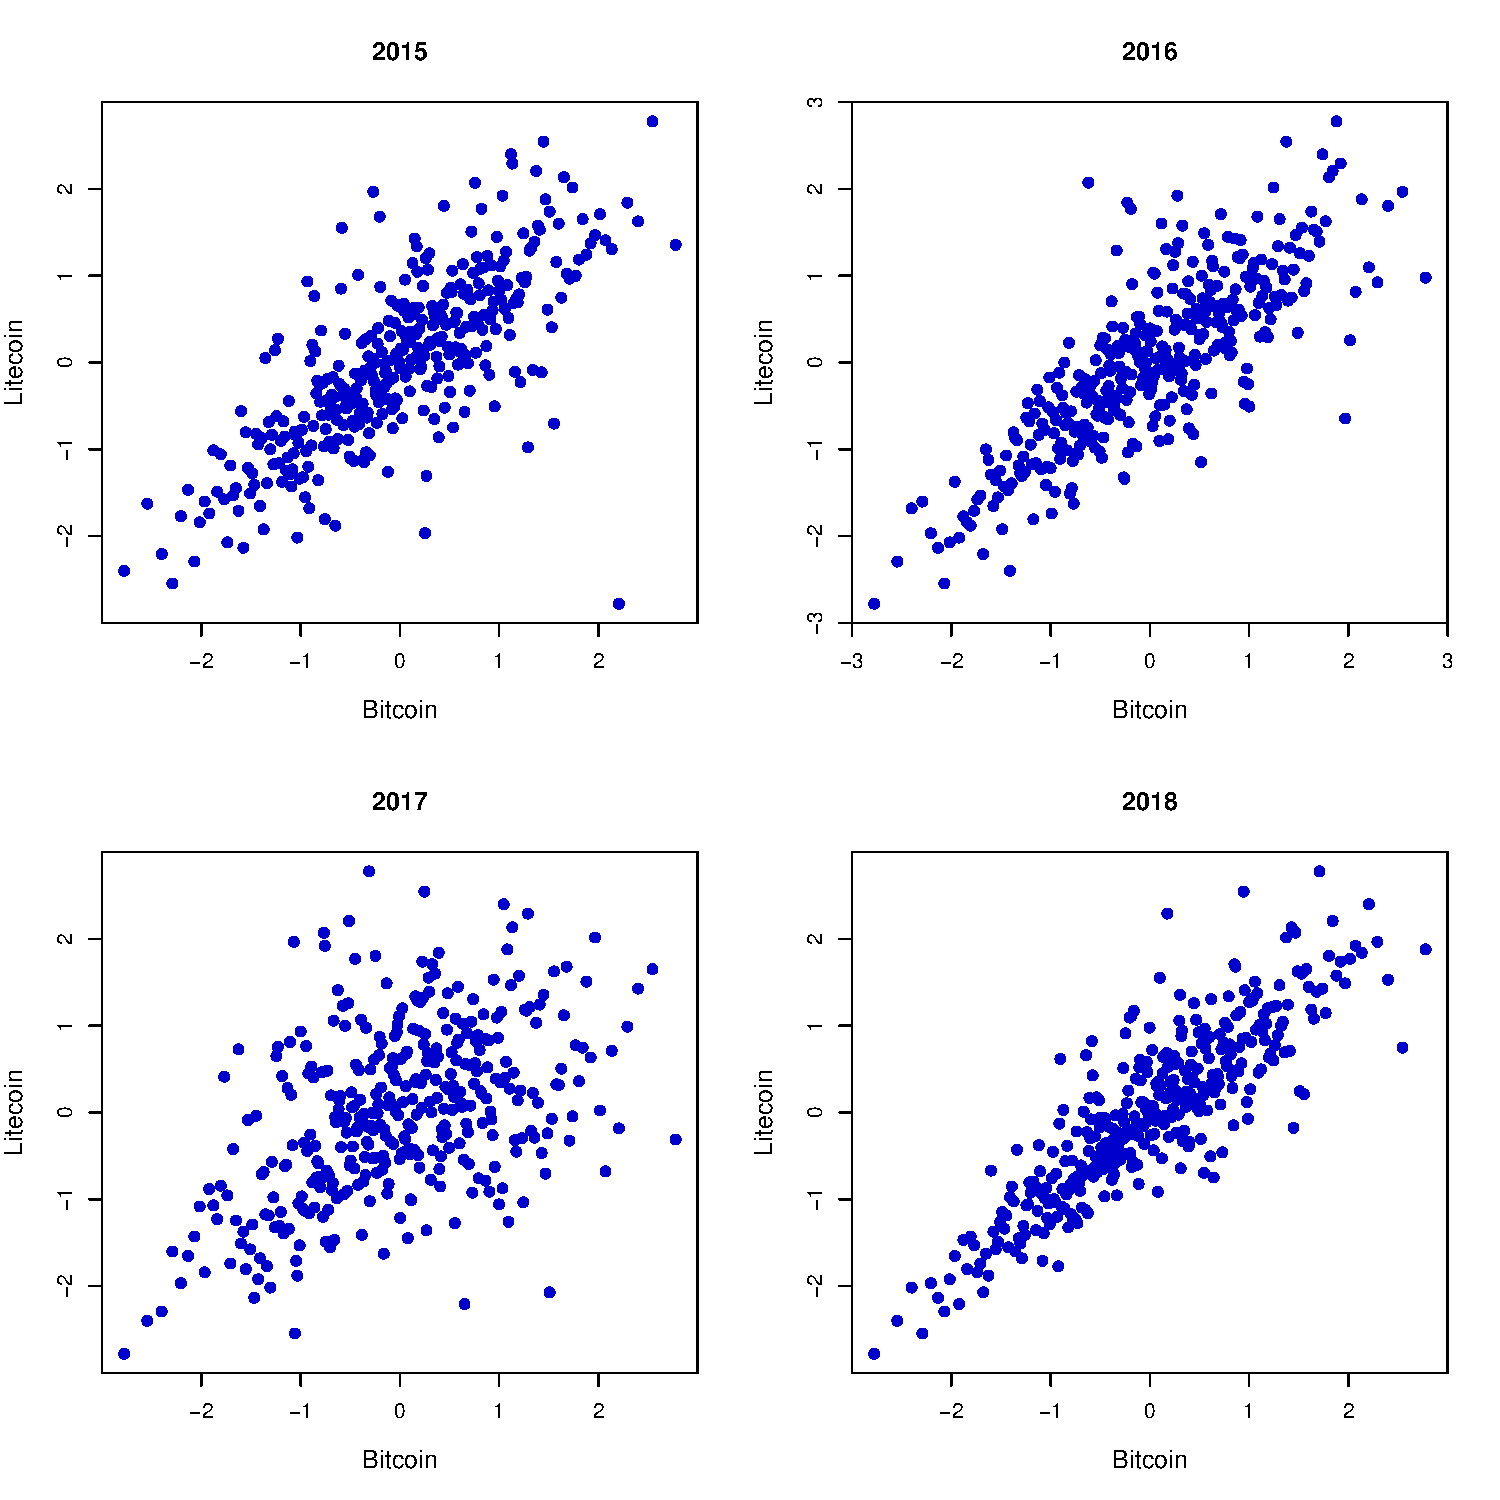
\includegraphics[width = 110mm]{img/BTC_LTC_Residuals.pdf}
	\caption{Residual plots for BTC-LTC with margins transformed to standard normal.}
	\label{Residual_BTC_LTC}
\end{figure}

\subsubsection{Goodness-of-fit testing}
\mycolor In this example, the focus in testing is on the most popular copula models in practice: normal, $t$, Clayton, Gumbel, and Frank copulae. To get the highest testing power, we include all tests, which are available for all five copulae. Thus, following Table \ref{tab:Combs_tests_cops_dims}, each test in the package except the ones based on the transformation for Archimedean copulae (see Section \ref{subsec:gof_Archm}) is computed. Additionally, all possible hybrid tests are considered. We use the function \code{gof} while setting the bootstrap parameters $M = 100$ and $MJ = 1000$. We specify the number of cores for the parallelization to \code{processes = 7}. For replicability, we set \code{seed.active = 1:101} and apply the non-parametric margin transformation by default.
\mycolor
\begin{example}
R> copulae = c("normal", "t", "clayton", "gumbel", "frank")

R> BTC_LTC_15 = gof(x = CryptoCurrencies[["2015"]], copula = copulae, M = 100, 
+                   MJ = 1000, processes = 7, seed.active = 1:101)
R> BTC_LTC_16 = gof(x = CryptoCurrencies[["2016"]], copula = copulae, M = 100, 
+                   MJ = 1000, processes = 7, seed.active = 1:101)
R> BTC_LTC_17 = gof(x = CryptoCurrencies[["2017"]], copula = copulae, M = 100, 
+                   MJ = 1000, processes = 7, seed.active = 1:101)
R> BTC_LTC_18 = gof(x = CryptoCurrencies[["2018"]], copula = copulae, M = 100, 
+                   MJ = 1000, processes = 7, seed.active = 1:101)
\end{example}
\bk
After finishing the calculations, we proceed by plotting the received objects of class \code{"gofCOP"}. For a detailed explanation about the information contained in the \pkg{gofCopula} pirateplots, please see Section \ref{subsec:gofCOP_plot} and \citet{phillips2017yarrr}.

\begin{example}
R> plot(BTC_LTC_15)
\end{example}
\vspace{-0.75cm}
\begin{figure}[H]
	\centering
 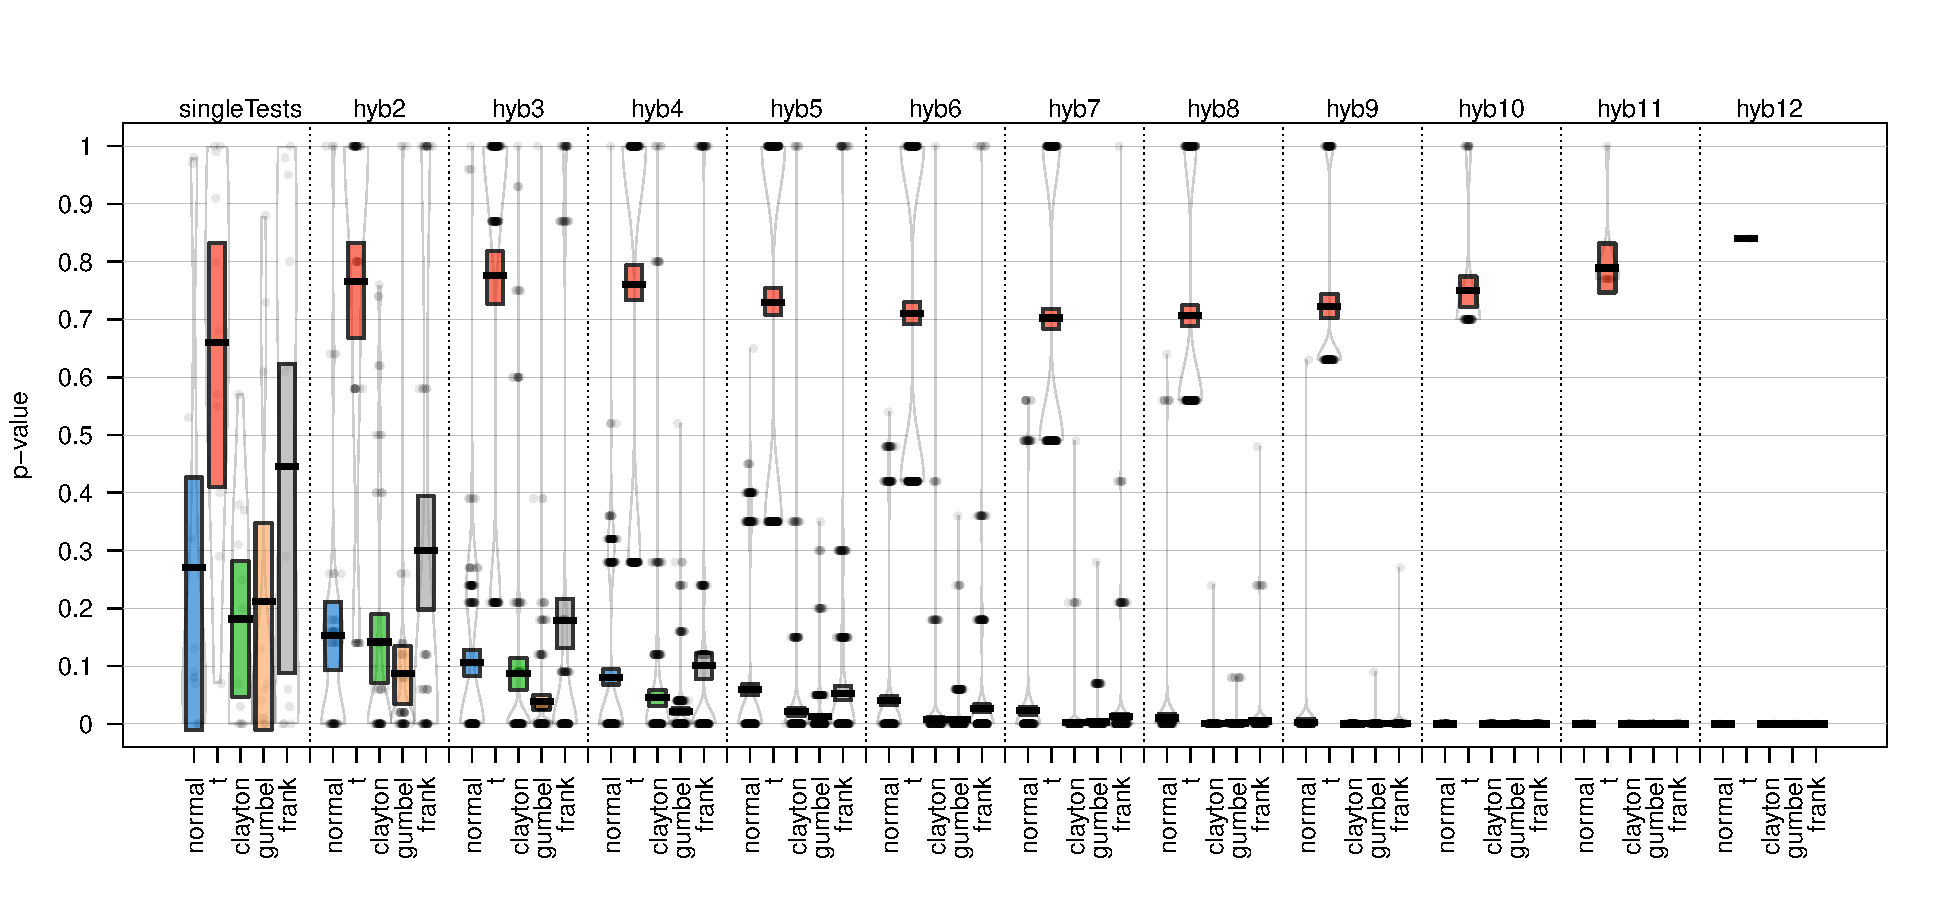
\includegraphics[width=\textwidth]{img/BTC_LTC_15.pdf}
	\caption{$p$-values of the single and hybrid tests for BTC-LTC in the year 2015.}
	\label{Pirateplot_BTC_LTC_15}
\end{figure}
\vspace{0.25cm}
\begin{example}
R> plot(BTC_LTC_16)
\end{example}
\vspace{-0.75cm}
\begin{figure}[H]
	\centering
 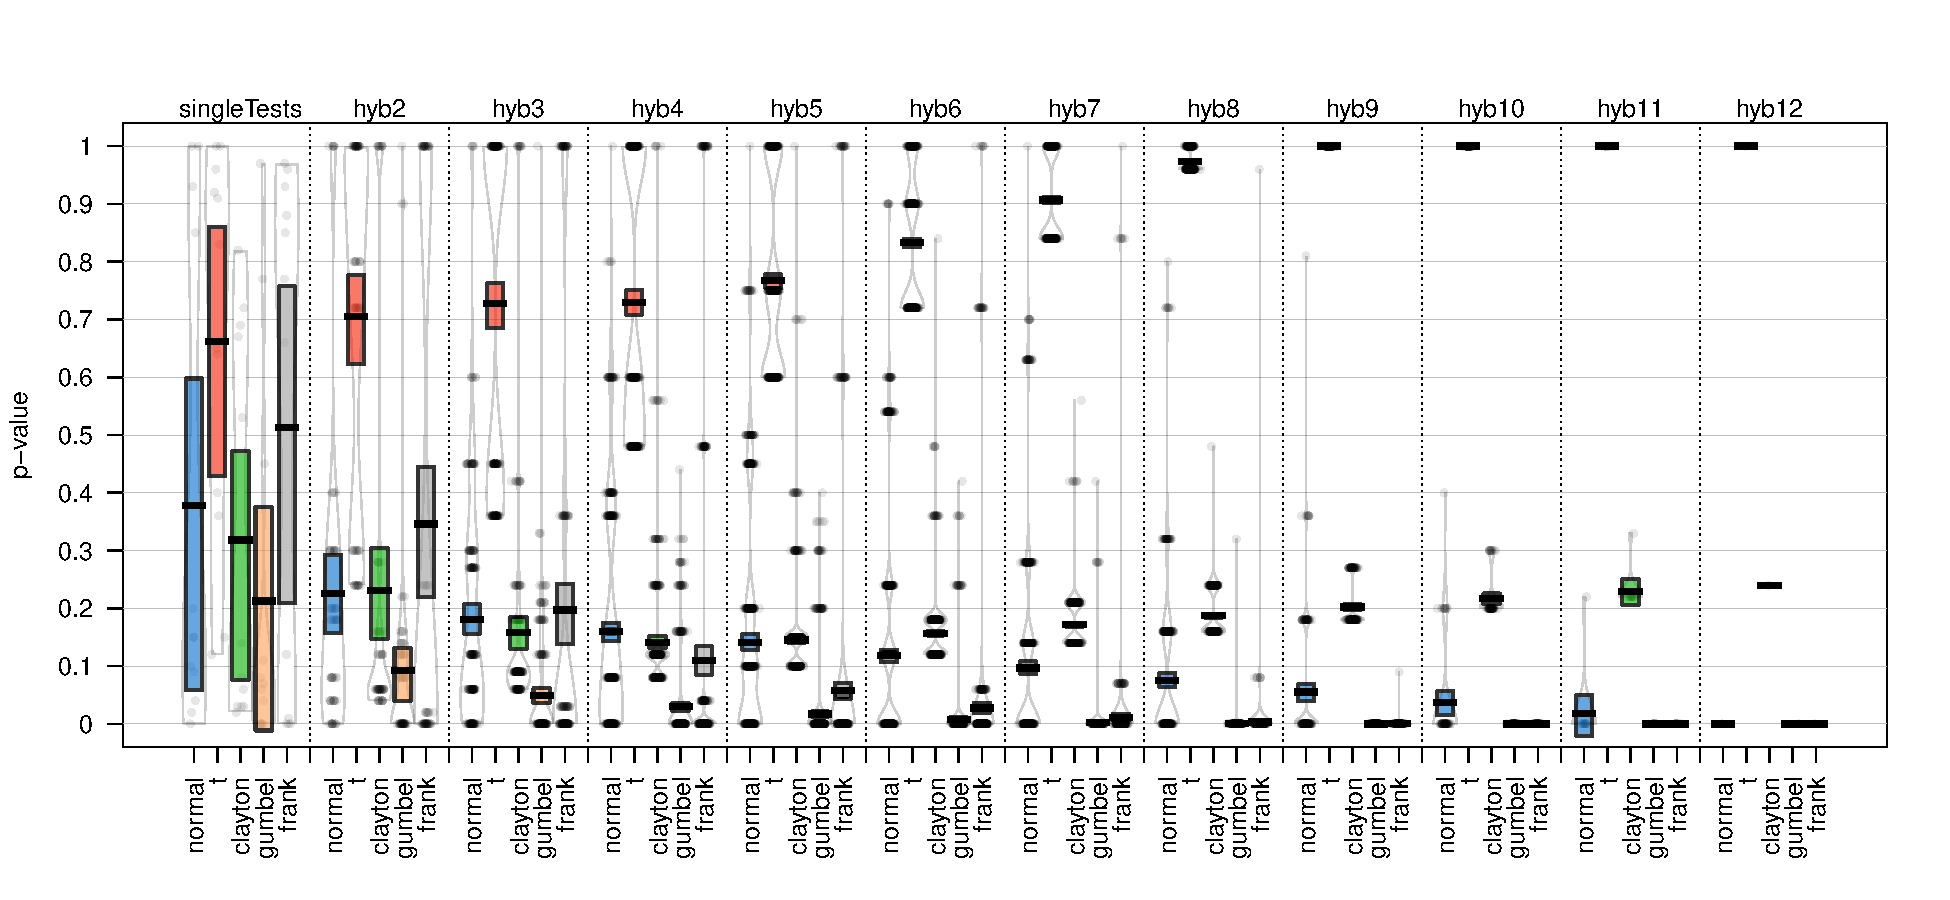
\includegraphics[width=\textwidth]{img/BTC_LTC_16.pdf}
	\caption{$p$-values of the single and hybrid tests for BTC-LTC in the year 2016.}
	\label{Pirateplot_BTC_LTC_16}
\end{figure}
\newpage
\begin{example}
R> plot(BTC_LTC_17)
\end{example}
\vspace{-1cm}
\begin{figure}[H]
	\centering
 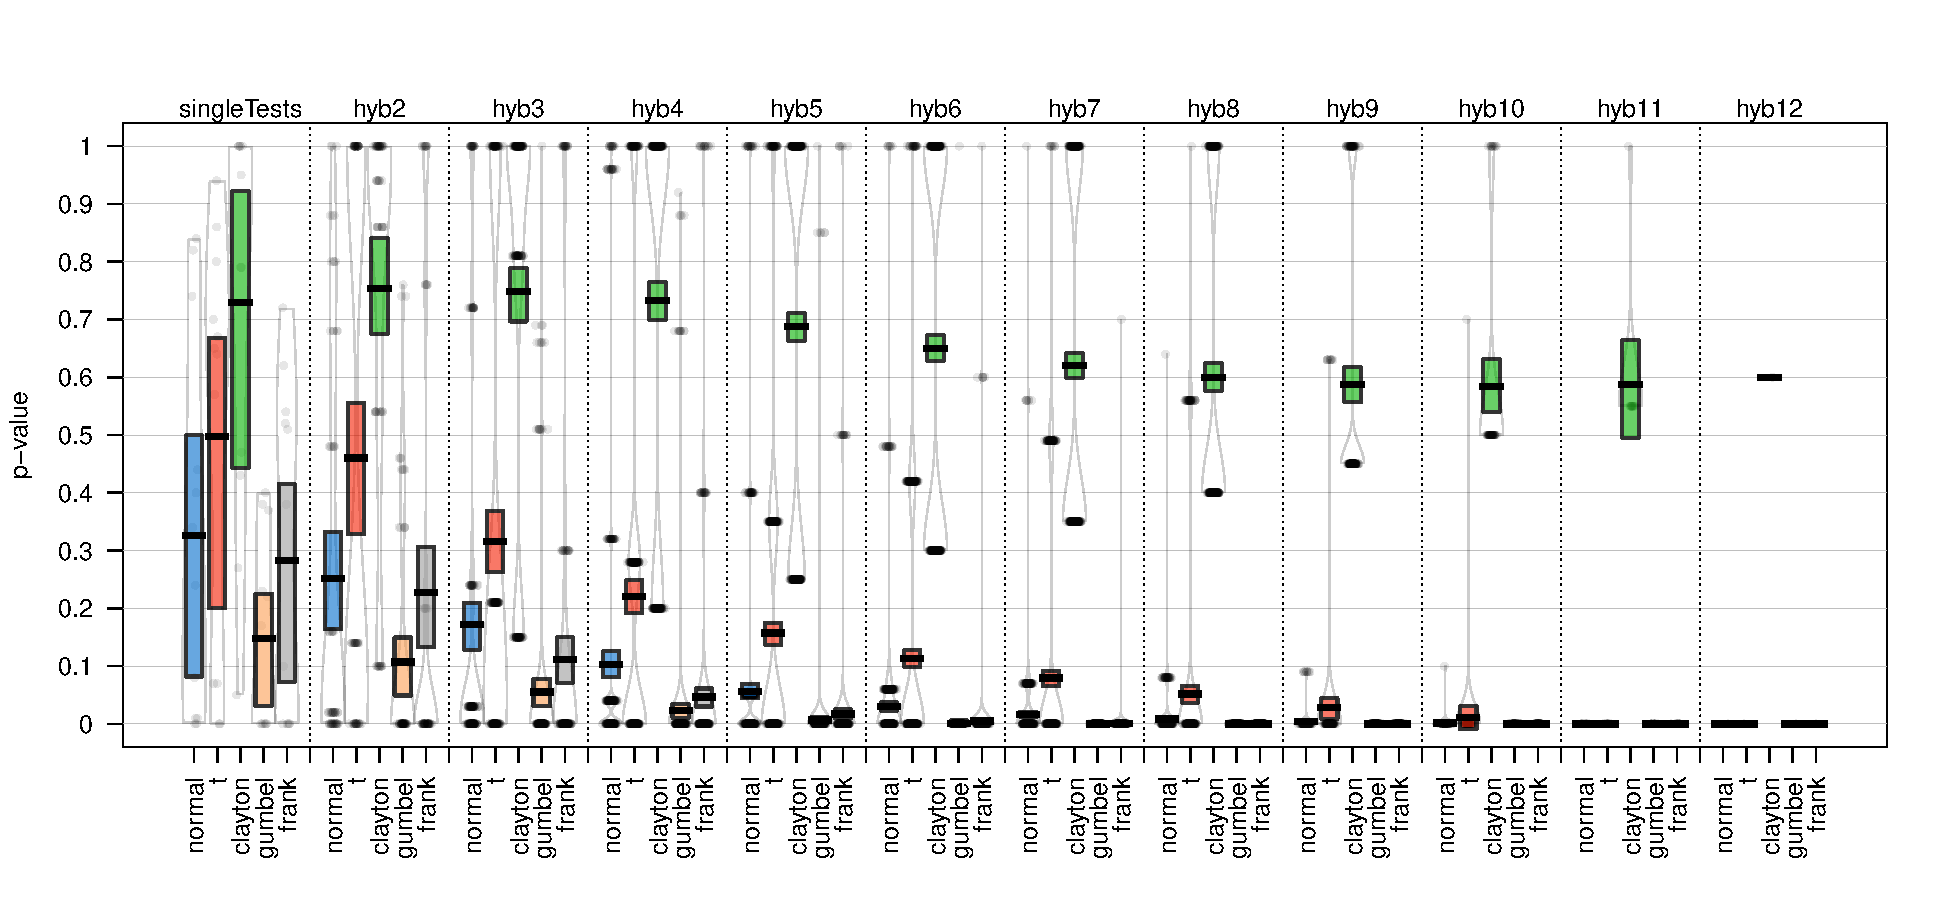
\includegraphics[width=\textwidth]{img/BTC_LTC_17.pdf}
	\caption{$p$-values of the single and hybrid tests for BTC-LTC in the year 2017.}
	\label{Pirateplot_BTC_LTC_17}
\end{figure}
\vspace{0.5cm}
\begin{example}
R> plot(BTC_LTC_18)
\end{example}
\vspace{-1cm}
\begin{figure}[H]
	\centering
 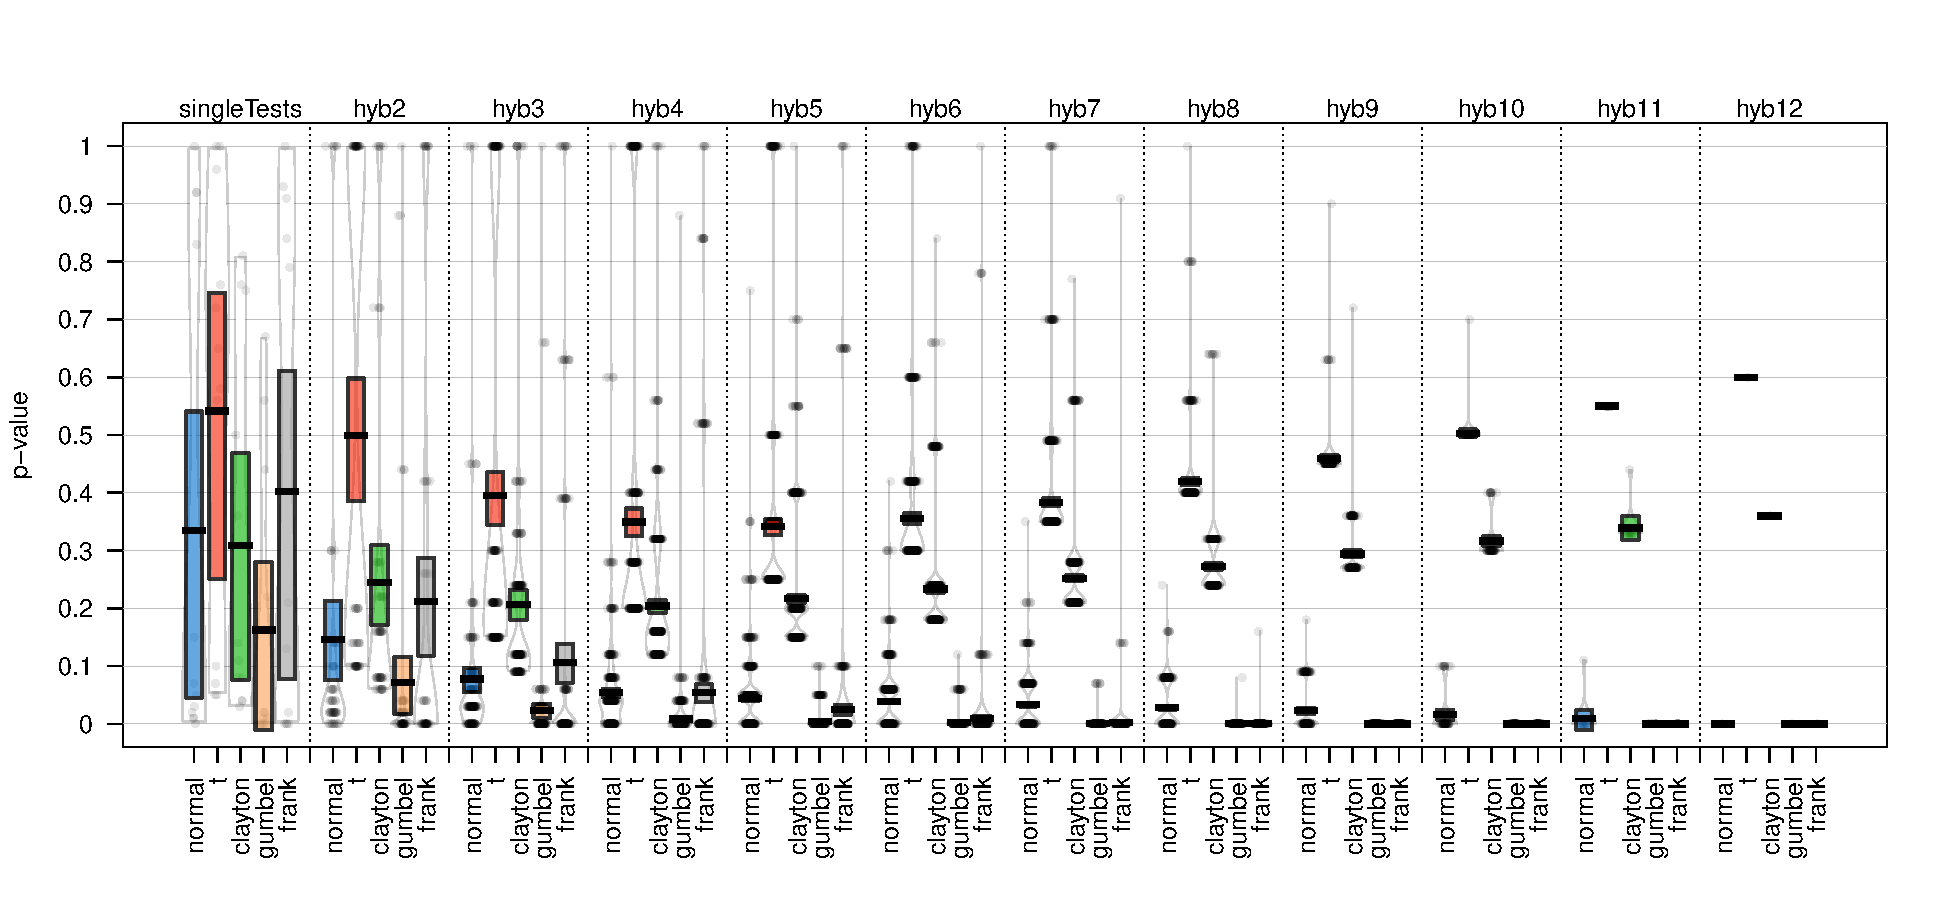
\includegraphics[width=\textwidth]{img/BTC_LTC_18.pdf}
	\caption{$p$-values of the single and hybrid tests for BTC-LTC in the year 2018.}
	\label{Pirateplot_BTC_LTC_18}
\end{figure}

Figures \ref{Pirateplot_BTC_LTC_15} to \ref{Pirateplot_BTC_LTC_18} show the resulting $p$-values in the form of \code{"gofCOP"}-plots for all the considered years. Following the usual approach in practice, we select the copula corresponding to the highest $p$-values. For the year 2015, we see that the $t$-copula is favored by the tests, as all remaining $p$-values become 0 with increasing hybrid testing size; \mycolor see Figure \ref{Pirateplot_BTC_LTC_15}. \bk This rejects our initial visual guess that a normal copula might be appropriate. Continuing with 2016, we see our visual opinion solidified, as the plot suggests using a $t$-copula to capture the dependence structure. We can even see that the $p$-values converge to 1 for the $t$-copula when we consider the hybrid testing orders \mycolor 9, 10, 11, and 12 \bk. Figure \ref{Pirateplot_BTC_LTC_17} is in line with our visual impression as well. We see that the tests favor a Clayton copula, while the other copula models are rejected by the higher-order hybrid tests. Finally, for 2018 Figure \ref{Pirateplot_BTC_LTC_18} gives for the $t$-copula the highest $p$-values, although the difference to the $p$-values of the Clayton copula is not too large. Therefore, in three out of four years, the results from \pkg{gofCopula} matched our visual impressions from the residual plots.

Summarizing, the following conclusions can be drawn from this analysis:
\begin{itemize}
    \item Generally, the dominant copulae in describing the dependency between the volatility-adjusted log-returns of BTC-LTC is the $t$-copula. Following the test results, the year 2017 is an exception, as the dependence structure shifted towards a Clayton copula. This observation reflects the change in the market during the year 2017, as many investors got attracted by cryptocurrencies in this phase. Due to the developed hype, both the prices of BTC and LTC drastically increased, resulting in a modified underlying dependence structure between the two currencies.
    \item The hybrid tests are able to stabilize the results of the single tests, as they clearly selected for 2015, 2016, and 2018 the $t$-copula and in 2017 the Clayton copula. Therefore it is recommendable to take hybrid tests into account in order to use the package adequately and get the highest testing power.
\end{itemize}

\subsection{Stock return data}
\label{subsec:C_BoA}
As a second real-world example, we analyze the volatility-adjusted stock log-returns of Citigroup (C) and the Bank of America (BoA) in the time span from 2004 to 2012. The procedure is, again, splitted into \emph{Data Investigation} and \emph{Goodness-of-Fit testing}.

\subsubsection{Data investigation}
\mycolor This data was analyzed by \citet{zhang_okhrin_song_zhou_2016}, and we are expanding their procedure and consider the same copulae and tests as in the example in Section \ref{subsec:Cryptos}. The volatility correction was performed similarly in terms of fitting a GARCH(1,1) process, and the resulting data is included in \pkg{gofCopula} in the list \code{Banks}. \bk Note that in this section, we focus on the years 2004 and 2007, while the results of the other years are given in Appendix \hyperref[sec:AppendixStock]{B}. We start by visualizing the residuals with margins transformed to standard normal.
\mycolor
\begin{example}
R> library("gofCopula")
R> data("Banks", package = "gofCopula")
R> par(mfrow = c(1,2))

R> for(i in c("2004", "2007")){
+     x1 = Banks[[i]][,1]
+     x2 = Banks[[i]][,2]
+      n = length(x1)
+     plot(qnorm(cbind(ecdf(x1)(x1), ecdf(x2)(x2)) * n / (n + 1)), col = "blue3", 
+     pch = 19, cex.lab = 1.25, main = i, xlab = "Citigroup", ylab = "Bank of America")
+  }
R> par(mfrow = c(1,1))
\end{example}
\bk
\begin{figure}[H]
	\centering
 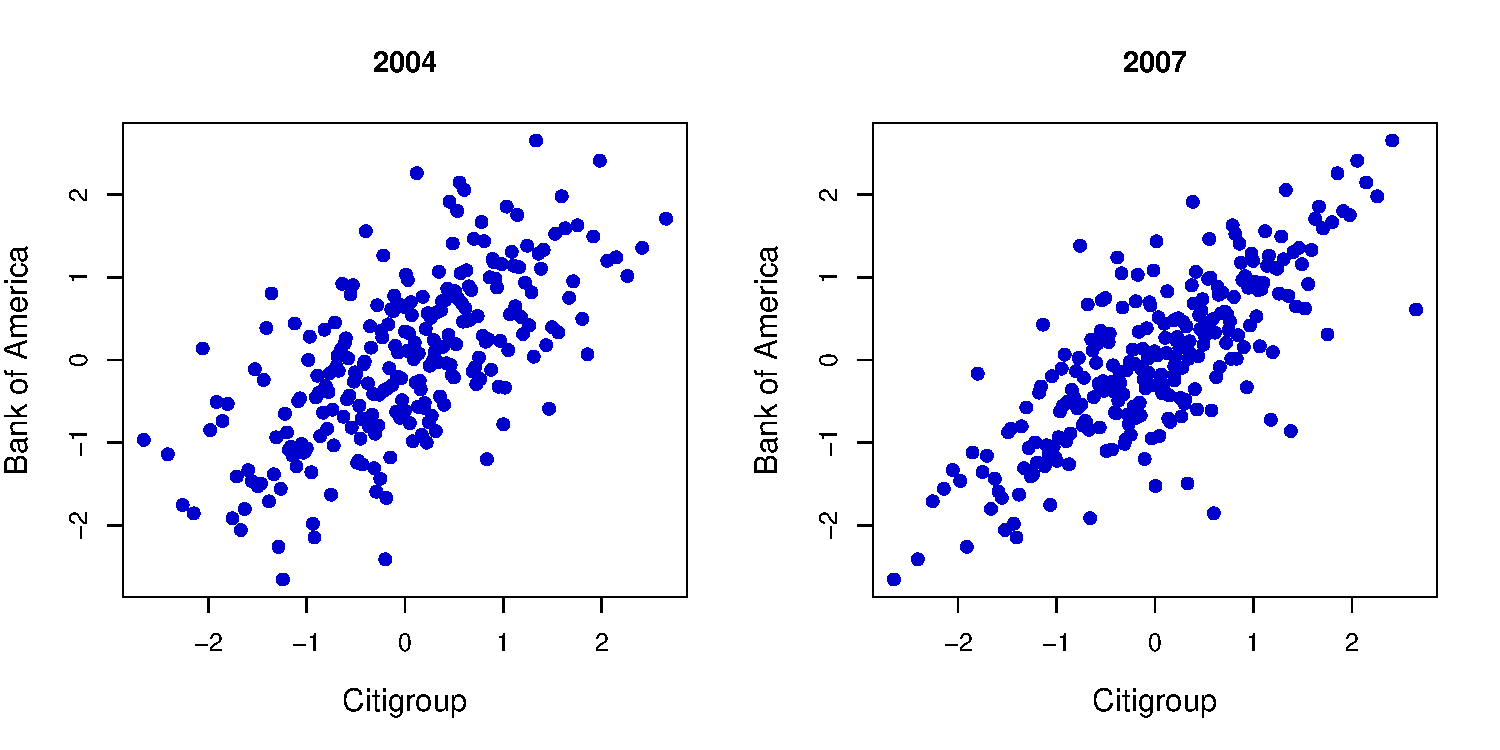
\includegraphics[width=\textwidth]{img/C_BoA_Residuals.pdf}
	\caption{Residual plots for C/BoA in 2004 and 2007 with standard normal margins.}
	\label{Residuals_C_BoA}
\end{figure}

Analyzing the shape of the data in Figure \ref{Residuals_C_BoA} for 2004, one may argue that the elliptical normal copula is present, while in 2007, a $t$-copula is possibly more appropriate. To check these assumptions, we proceed with the GoF testing.

\subsubsection{Goodness-of-fit testing}
\mycolor We set \code{M = 100} and \code{MJ = 1000} as bootstrap parameters, parallelize via \code{processes = 7}, and set \code{seed.active = 1:101} for reproducibility. Further, we implicitly keep the default \verb'margins = "ranks"' to perform the margin transformation nonparametrically.

\begin{example}
R> copulae = c("normal", "t", "clayton", "gumbel", "frank")

R> C_BoA_04 = gof(x = Banks[["2004"]], copula = copulae, M = 100, MJ = 1000, 
+                 processes = 7, seed.active = 1:101)
R> C_BoA_07 = gof(x = Banks[["2007"]], copula = copulae, M = 100, MJ = 1000, 
+                 processes = 7, seed.active = 1:101)
\end{example}

Following these calculations, we continue to plot the results, leading to Figures \ref{Pirateplot_C_BoA_04} and \ref{Pirateplot_C_BoA_07}. For a detailed explanation about the information contained in the \pkg{gofCopula} pirateplots, please see Section \ref{subsec:gofCOP_plot} and \citet{phillips2017yarrr}. Interpreting these \code{"gofCOP"}-plots of the $p$-values, the tests propose for 2004 indeed a normal copula (and a Frank one, which is \mycolor radially symmetric\bk), although a $t$-copula is a valid assumption as well. Compared to 2004, the $p$-values for the normal copula definitely decreased in 2007 and converged slowly to 0 with increasing hybrid testing size. The decision goes clearly in favor of the $t$-copula, which is in line with our original guess. Evaluating the results from Appendix \hyperref[sec:AppendixStock]{B} leads to similar conclusions as in Section \ref{subsec:Cryptos}. The hybrid tests are relatively stable and match in the majority of the cases the visual impressions from the residual plots. The proper copula seems to be the $t$-copula in most of the years, although in 2004 and 2009, the normal copula is a reasonable assumption. The hybrid tests are able to stabilize the selection of the copula.\\

\begin{example}
R> plot(C_BoA_04)
\end{example}
\vspace{-1cm}
\begin{figure}[H]
	\centering
 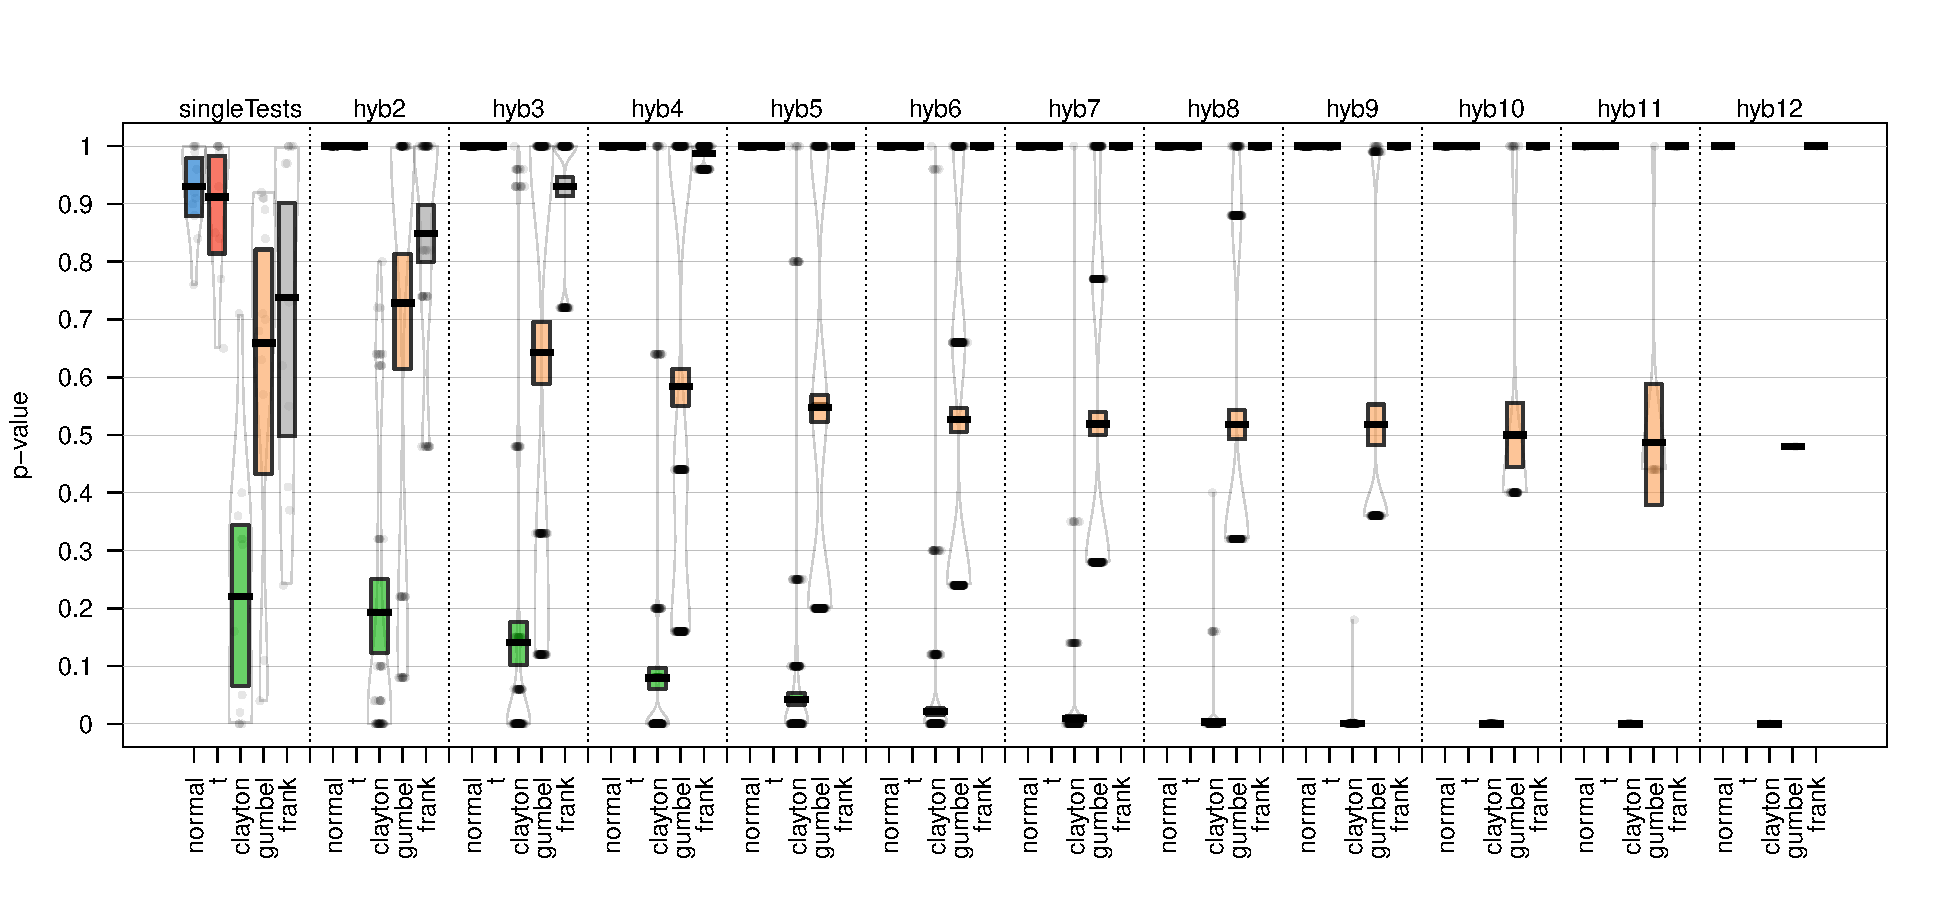
\includegraphics[width=\textwidth]{img/C_BoA_04.pdf}
	\caption{$p$-values of the C/BoA data for 2004. The column \mycolor \protect\code{hyb12} \bk of the $t$-copula is empty, as the $p$-value of the test \protect\code{gofWhite} could not be computed due to instability in the test statistics. For a detailed description of this phenomenon, see \citet{schepsmeier2018package}.}
	\label{Pirateplot_C_BoA_04}
\end{figure}

\vspace{0.25cm}
\begin{example}
R> plot(C_BoA_07)
\end{example}
\vspace{-1cm}
\begin{figure}[H]
	\centering
 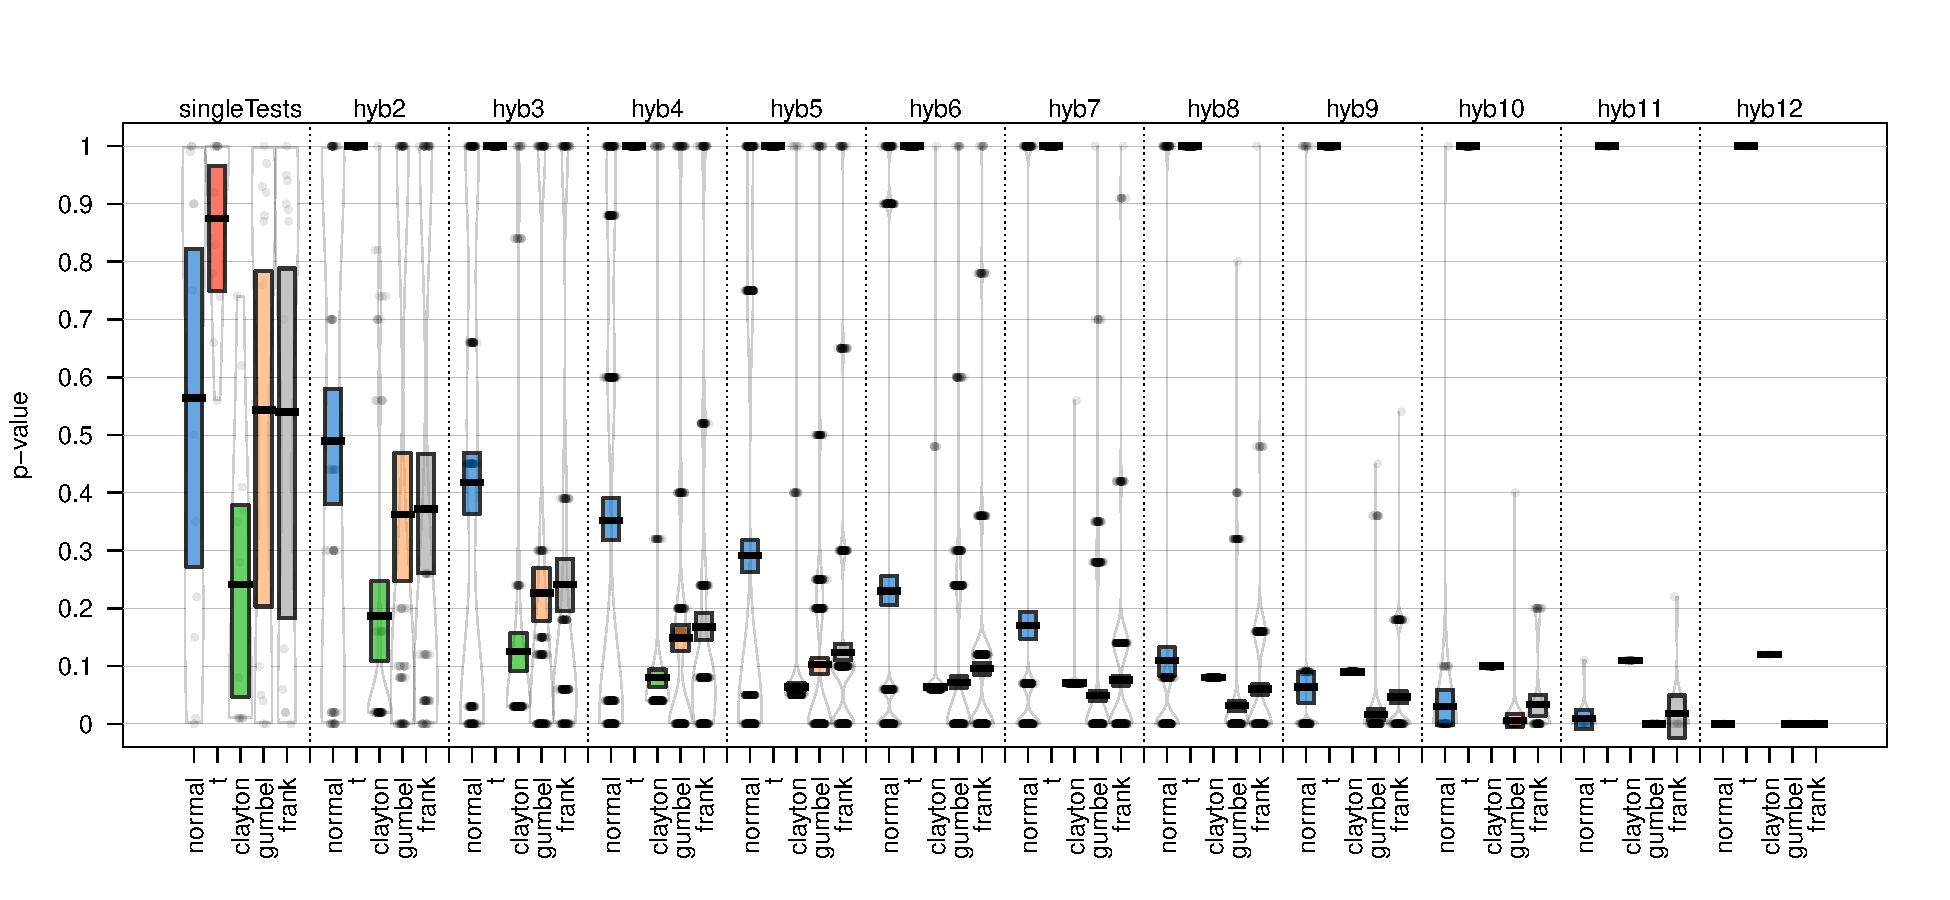
\includegraphics[width=\textwidth]{img/C_BoA_07.pdf}
	\caption{$p$-values of the C/BoA data for 2007.}
	\label{Pirateplot_C_BoA_07}
\end{figure}

\section{Conclusion}
\label{sec:conclusion}
This paper introduces a \pkg{gofCopula} package that provides maximum flexibility in performing statistical Goodness-of-Fit tests for copulae. The package provides an interface for \mycolor 16 most popular GoF tests for 13 copulae with automatic estimation of margins via different techniques. \bk The user is not limited to the implemented tests as self-defined test statistics functions can be easily embedded via a function provided in the package. As the computation of $p$-values relies on a parametric bootstrap, efficient and user-friendly parallelization is available. During the bootstrapping procedure, all tests inform the user about the progress of the calculations as well as the estimated time until the results are available. Additionally, \pkg{gofCopula} allows for the replication of said results. The package offers intelligible and interpretable visualization of the results of the hybrid tests that strengthen the overall test power. The flexibility and the usefulness of the tests are shown via a simulation and two empirical studies in economic sciences. In a nutshell, the broad range of tests, the comprehensive combination of methods, and an informative user-interface make \pkg{gofCopula} a fire-and-forget package providing flexibility in testing for the proper copula.\\

\section{Acknowledgements}
The authors are grateful to Shulin Zhang, Qian Zhou, Peter Song, and \mycolor Sören Pannier \bk for helpful discussions and to Oliver Scaillet for the code of the version of his test used in \citet{zhang_okhrin_song_zhou_2016} that is being adapted in this package. Financial support from NUS FRC grant R-146-000-298-114 ``Augmented machine learning and network analysis with applications to cryptocurrencies and blockchains'' \mycolor as well as CityU Start-Up Grant 7200680 ``Textual Analysis in Digital Markets'' \bk is gratefully acknowledged by Simon Trimborn. Ostap Okhrin thankfully received financial support from RFBR, project number 20-04-60158.

\bibliography{okhrin-trimborn-waltz.bib}

\newpage
\begin{appendices}
\renewcommand\thetable{A.\arabic{table}}
\renewcommand\thefigure{A.\arabic{figure}}
\setcounter{table}{0}
\renewcommand{\thesubsection}{A.\arabic{subsection}}

\section{Appendix A}\label{sec:Appendix:cop}
\mycolor Table \ref{tbl:copula_characteristics} contains parameter ranges, the bivariate cumulative distribution function (CDF), and possible values of Kendall's $\tau$ for the copulae available in \pkg{gofCopula}.\bk
\begin{table}[H]
\mycolor
\centering
 \begin{adjustbox}{max width=\textwidth}
\begin{tabular}{lccc}
\toprule
Copula & $\theta \in$ & $C(u_1, u_2)$ & $\tau \in$\\
\midrule
\vspace{0.35cm}
Normal & $[-1,1]$ & $\int_{-\infty}^{\Phi^{-1}(u_1)} \int_{-\infty}^{\Phi^{-1}(u_2)} \frac{1}{2\pi \sqrt{1-\theta^2}} \exp{\left\{\frac{2\theta s t - s^2 -t^2}{2(1-\theta^2)}\right\}} \,ds dt$ & $[-1,1]$\\
\vspace{0.35cm}
$t$ & \makecell{$[-1,1]$ \\ $\nu > 0$} & $\int_{-\infty}^{t_{\nu}^{-1}(u_1)} \int_{-\infty}^{t_{\nu}^{-1}(u_2)} \frac{1}{2\pi \sqrt{1-\theta^2}} \left\{1 + \frac{s^2+t^2-2\theta s t}{\nu(1-\theta^2)}\right\}^{-\frac{\nu+2}{2}} ds dt$ & $[-1,1]$\\
\vspace{0.35cm}
Clayton & $[-1,\infty) \backslash \{0\}$ & $\left\{\max(u_1^{-\theta} + u_2^{-\theta} - 1,0)\right\}^{-\frac{1}{\theta}}$ & $[-1,1]$\\
\vspace{0.35cm}
Gumbel & $[1,\infty)$ & $\exp{\left[ - \left\{ (-\log u_1)^{\frac{1}{\theta}} + (-\log u_2)^{\frac{1}{\theta}}  \right\}^{\theta} \right]}$ & $[0,1]$\\
\vspace{0.35cm}
Frank & $(-\infty, \infty) \backslash \{0\}$ & $-\frac{1}{\theta} \log \left[1+ \frac{\{\exp(-\theta u_1) - 1\}\{\exp(-\theta u_2) - 1\}} {\exp(-\theta) - 1} \right]$ & $[-1,1]$\\
\vspace{0.35cm}
Joe & $[1,\infty)$ & $1- \left\{ (1-u_1)^{\theta} + (1-u_2)^{\theta} - (1-u_1)^{\theta}(1-u_2)^{\theta} \right\}^{\frac{1}{\theta}}$ & $[0,1]$\\
\vspace{0.35cm}
AMH & $[-1,1]$ & $\frac{u_1 u_2}{1-\theta (1-u_1)(1-u_2)}$ & \makecell{$[\frac{5 - 8 \log 2}{3}, \frac{1}{3}]$\\ $\approx [-0.1817, 0.3333]$}\\
\vspace{0.35cm}
Galambos & $[0,\infty)$ & $u_1 u_2 \exp \left[ \left\{ (-\log u_1)^{-\theta} + (-\log u_2)^{-\theta} \right\}^{-\frac{1}{\theta}}\right]$ & $[0,1]$ \\
\vspace{0.35cm}
Husler-Reiss & $[0,\infty)$ & $\exp \left\{ \log(u_1) \Phi (\frac{1}{\theta} + \frac{1}{2} \theta \log \frac{\log u_1}{\log u_2}) + \log(u_2) \Phi (\frac{1}{\theta} + \frac{1}{2} \theta \log \frac{\log u_2}{\log u_1}) \right\}$ & $[0,1]$\\
\vspace{0.35cm}
Tawn & $[0,1]$ & $u_1 u_2 \exp \left( -\theta \frac{\log u_1 \log u_2}{\log u_1 + \log u_2}\right)$ & \makecell{$[0,\frac{8 \arctan (\sqrt{\frac{1}{3})}}{\sqrt{3}}-2]$\\ $\approx [0,0.4184]$}\\
\vspace{0.35cm}
$t$-EV & \makecell{$[-1,1]$ \\ $\nu > 0$} & see \cite{demarta_mcneil_2004} & $[0,1]$ \\
\vspace{0.35cm}
FGM & $[-1,1]$ & $u_1 u_2 + u_1 u_2 \theta (1-u_1)(1-u_2)$ & $[-\frac{2}{9}, \frac{2}{9}]$\\
\vspace{0.35cm}
Plackett & $(0,\infty)$ & $\frac{ \left\{ 1+(\theta-1)(u_1+u_2)\right\} - \sqrt{\left\{ 1+(\theta -1)(u_1+u_2)\right\}^{2} -4 u_1 u_2 \theta (\theta-1)} }{2(\theta-1)}$ & $[-1,1]$ \\
\bottomrule
\end{tabular}
\end{adjustbox}
\caption{\mycolor This table is mainly based on \cite{michiels2008copula}. AMH abbreviates Ali-Mikhail-Haq. FGM stands for Farlie-Gumbel-Morgenstern. $\Phi$ is the CDF of the univariate standard normal distribution and $\Phi^{-1}$ its inverse. $t_{\nu}^{-1}$ is the inverse CDF of the univariate $t$-distribution with $\nu$ degrees of freedom. The expression of the CDF for the $t$-EV is complex due to the construction via a Pickands dependence function, which is why we do not explicitly list it. The given parameterization of the tawn copula is based on the one implemented in the package \pkg{copula}.}
\label{tbl:copula_characteristics}
\end{table}

\renewcommand\thefigure{B.\arabic{figure}}
\setcounter{figure}{0}
\section{Appendix B}
\label{sec:AppendixStock}
This section is devoted to the results of Section \ref{subsec:C_BoA}.
\vspace{-0.5cm}
\begin{figure}[H]
	\centering
 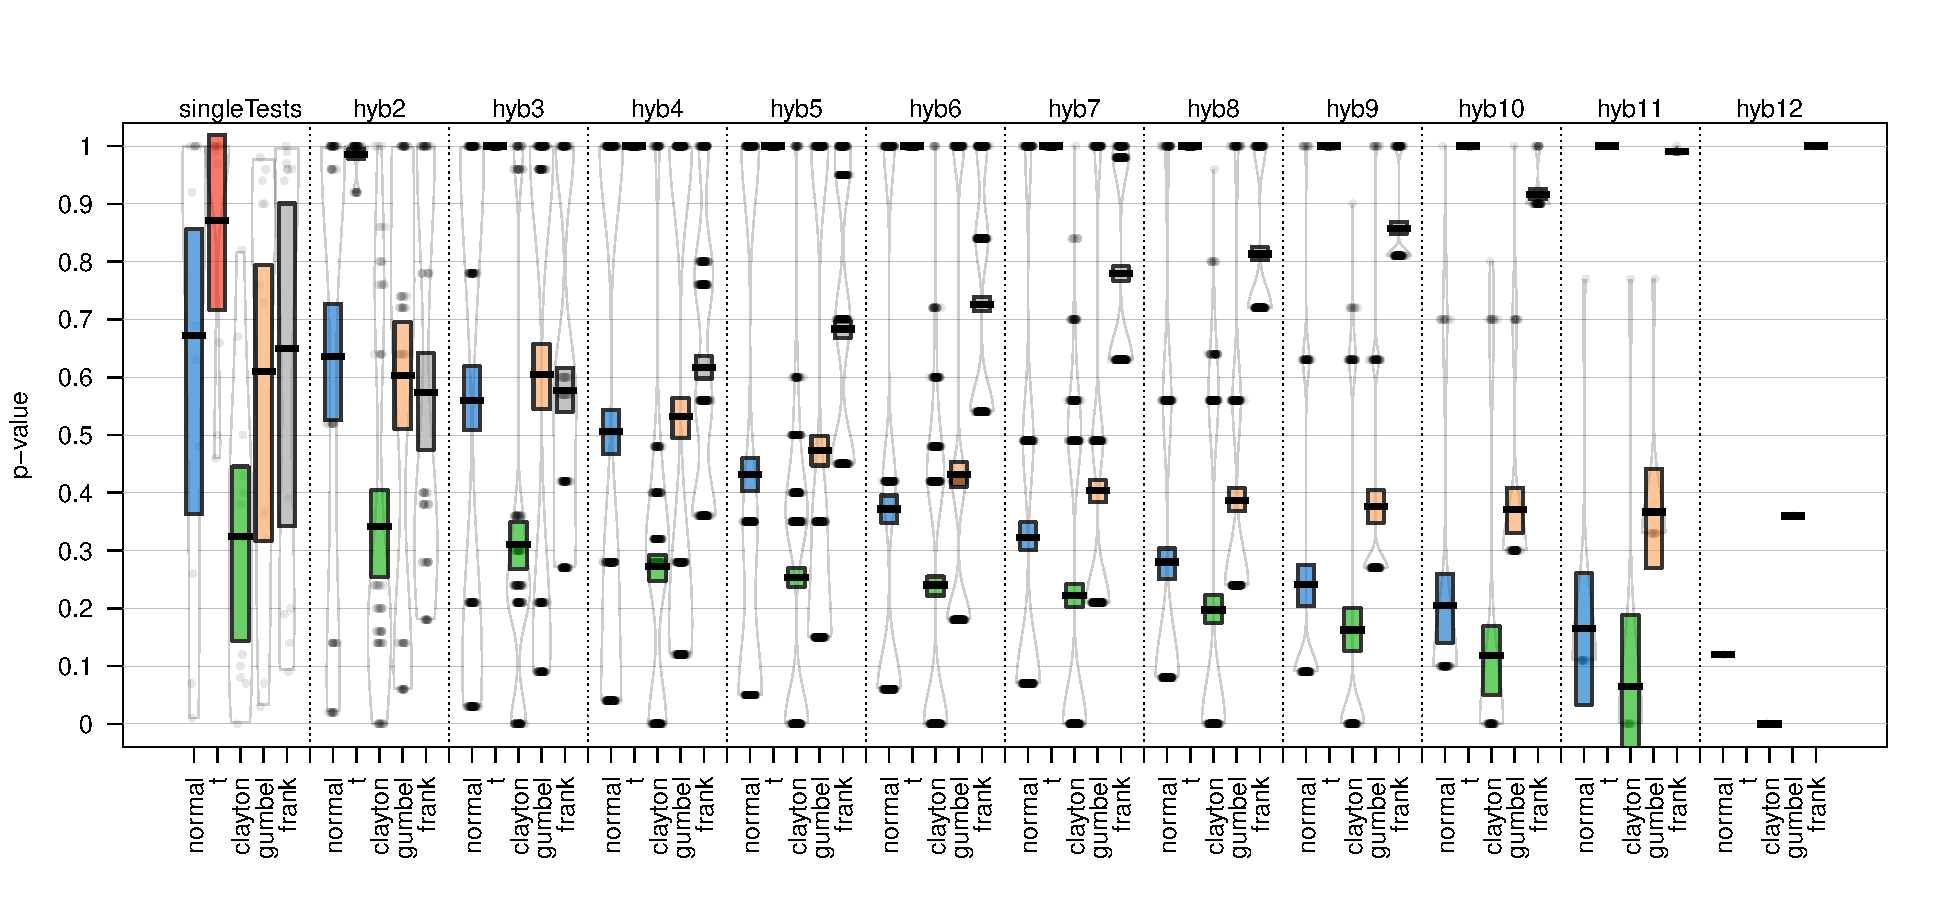
\includegraphics[width=\textwidth]{img/C_BoA_05.pdf}
	\caption{$p$-values of the C/BoA data for 2005. The column \mycolor \protect\code{hyb12} \bk of the $t$-copula is empty, as the $p$-value of the test \protect\code{gofWhite} could not be computed due to instability in the test statistics. For a detailed description of this phenomenon, see \citet{schepsmeier2018package}.}
	\label{Pirateplot_C_BoA_05}
\end{figure}
\vspace{-0.5cm}
\begin{figure}[H]
	\centering
 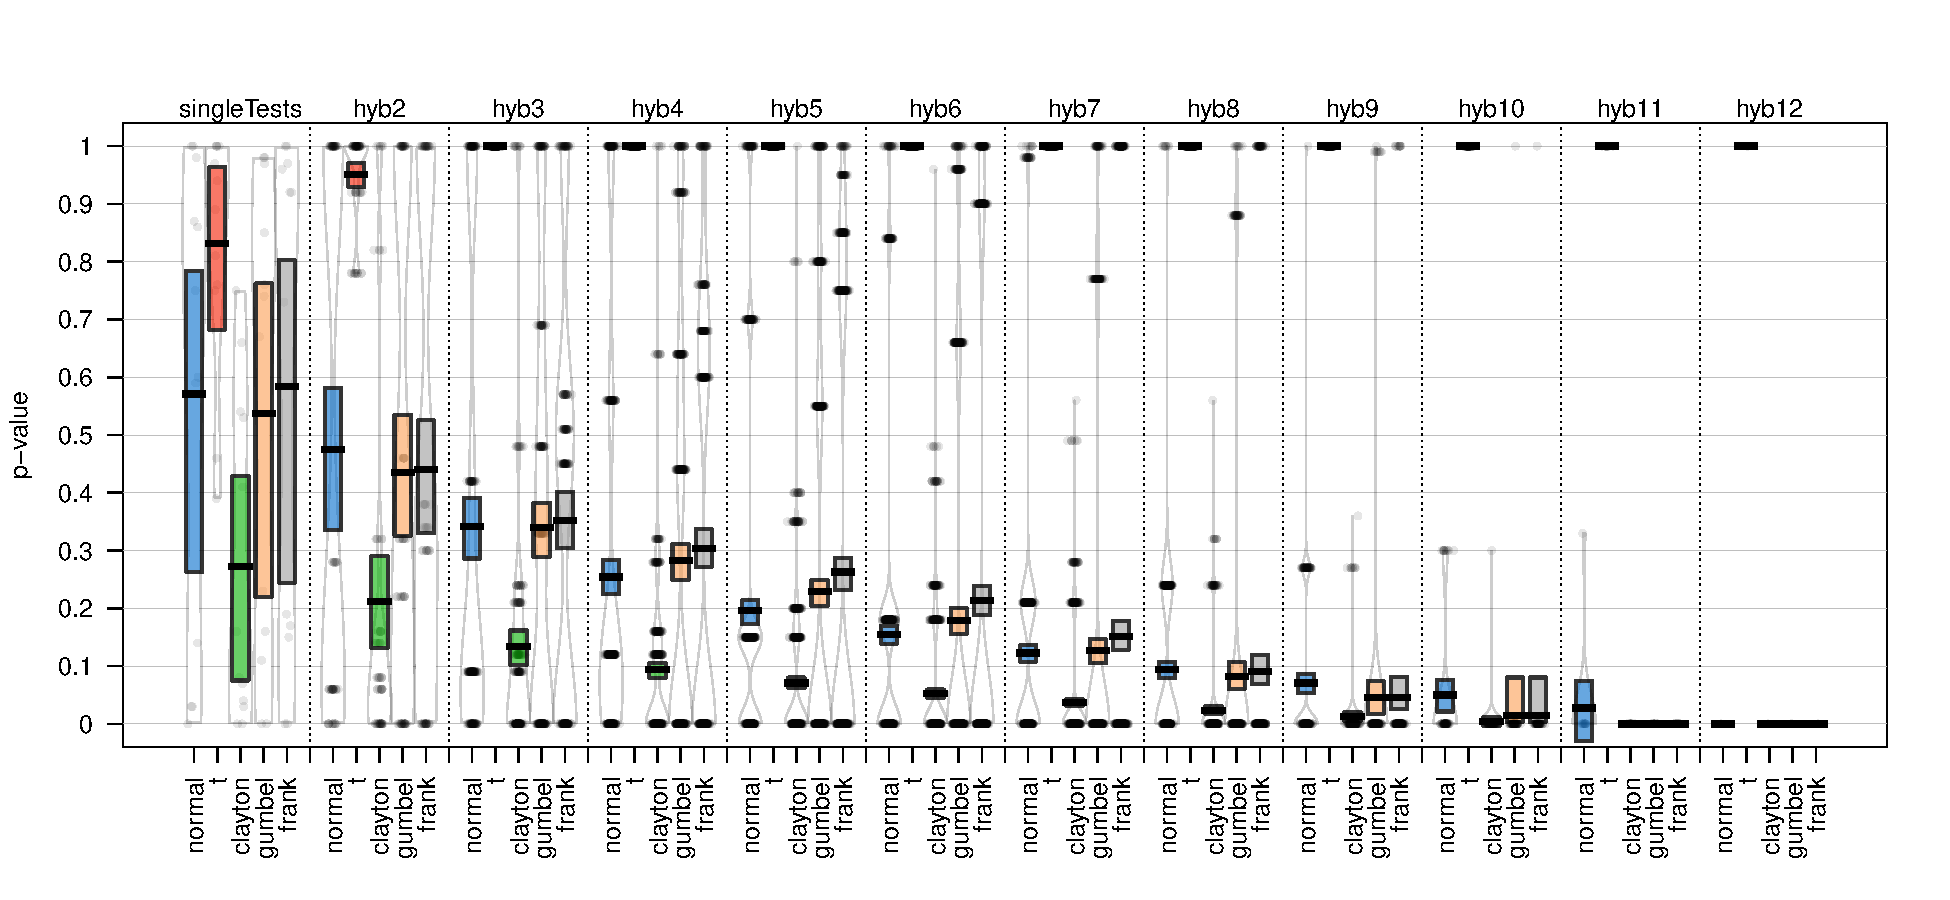
\includegraphics[width=\textwidth]{img/C_BoA_06.pdf}
	\caption{$p$-values of the C/BoA data for 2006.}
	\label{Pirateplot_C_BoA_06}
\end{figure}
\vspace{-0.5cm}
\begin{figure}[H]
	\centering
 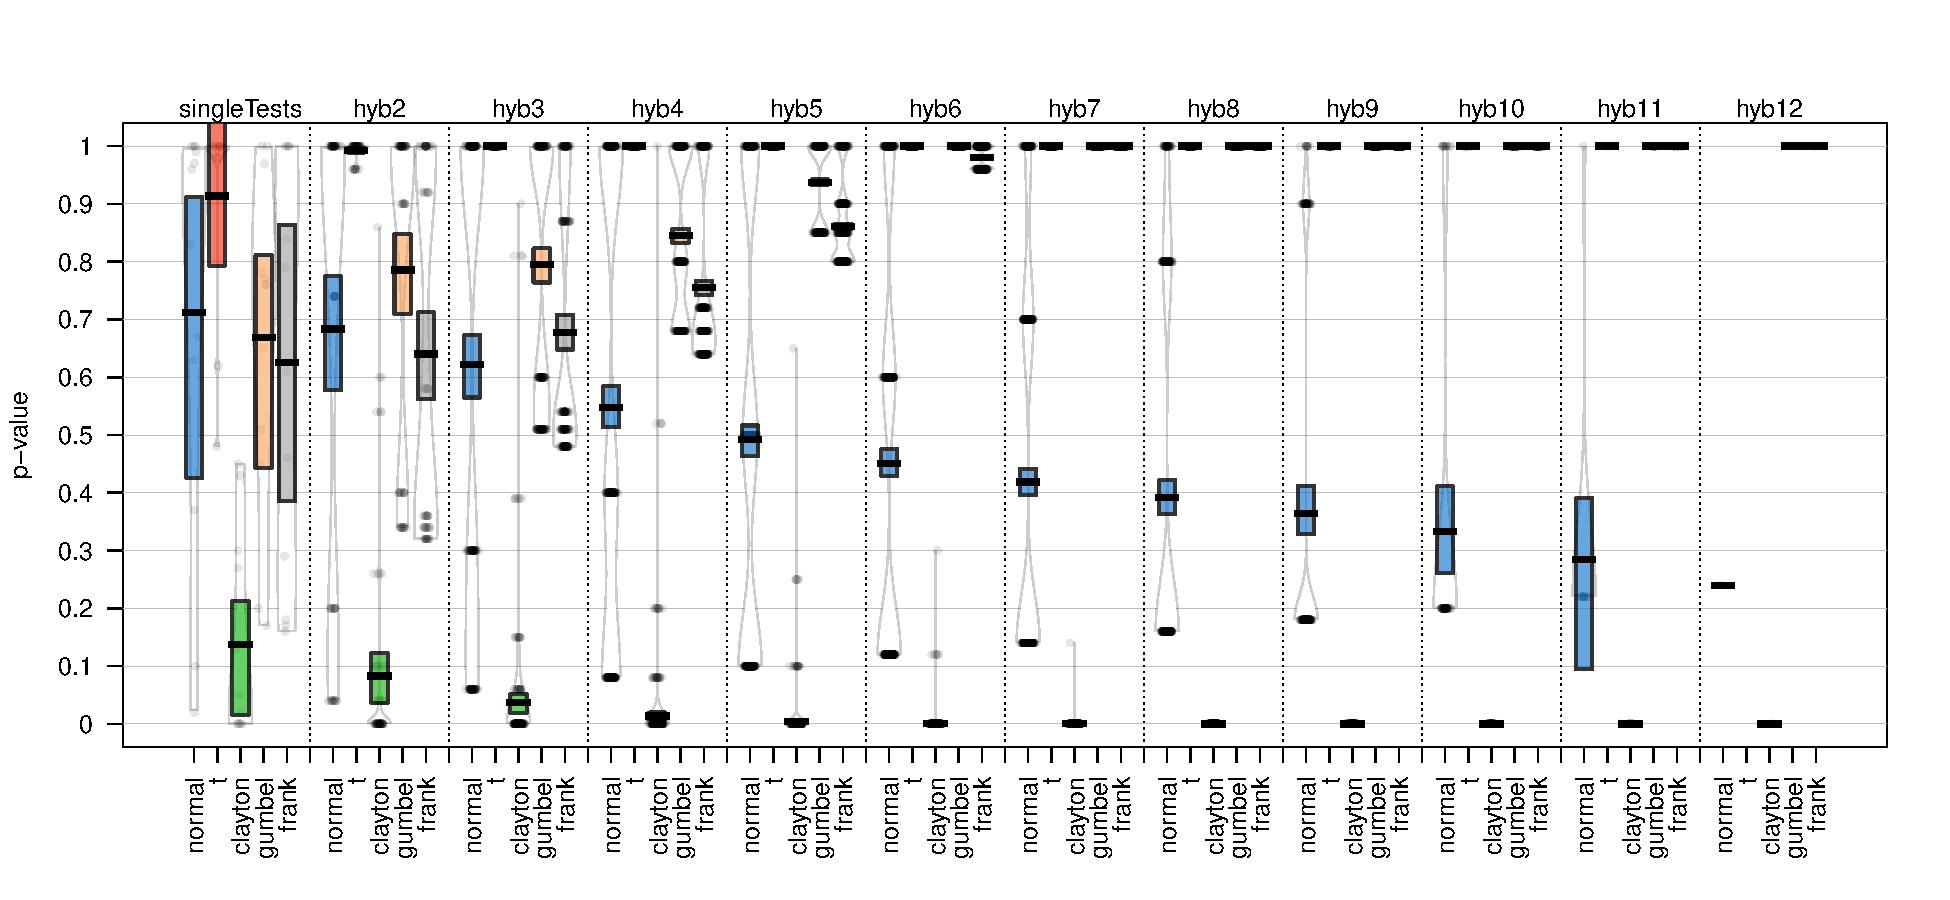
\includegraphics[width=\textwidth]{img/C_BoA_08.pdf}
	\caption{$p$-values of the C/BoA data for 2008. The column \mycolor \protect\code{hyb12} \bk of the $t$-copula is empty, as the $p$-value of the test \protect\code{gofWhite} could not be computed due to instability in the test statistics. For a detailed description of this phenomenon, see \citet{schepsmeier2018package}.}
	\label{Pirateplot_C_BoA_08}
\end{figure}
\vspace{-0.5cm}
\begin{figure}[H]
	\centering
 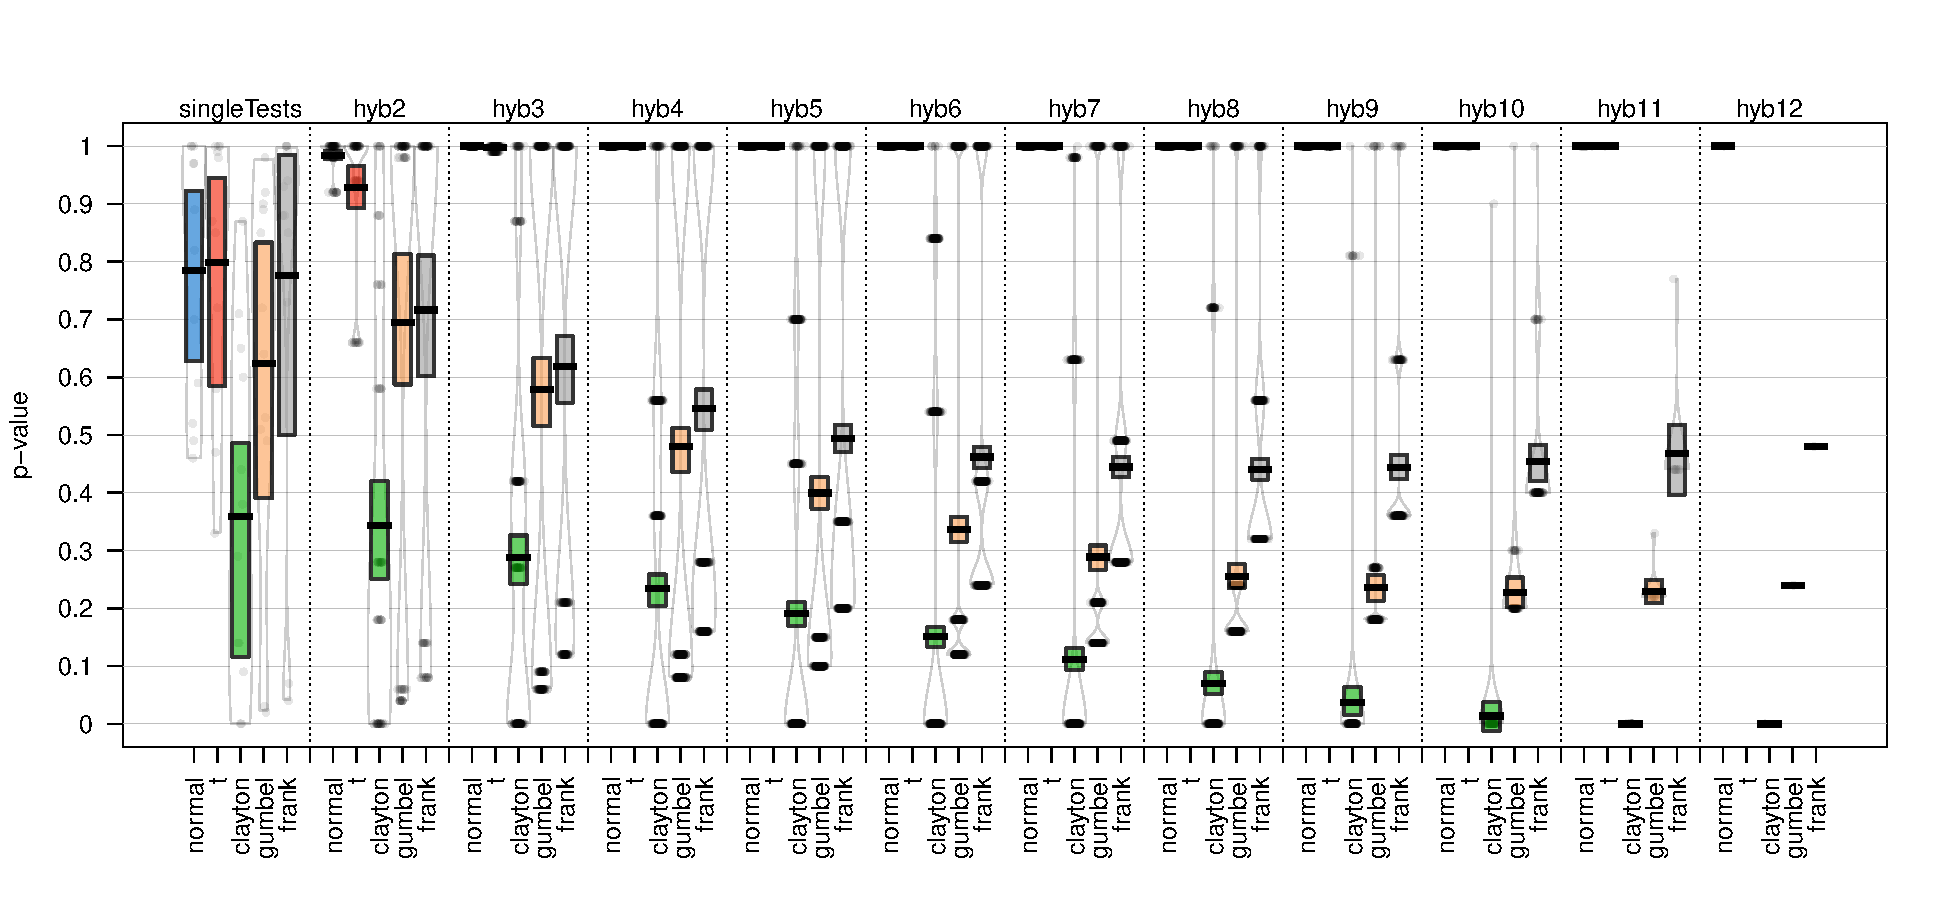
\includegraphics[width=\textwidth]{img/C_BoA_09.pdf}
	\caption{$p$-values of the C/BoA data for 2009. The column \mycolor \protect\code{hyb12} \bk of the $t$-copula is empty, as the $p$-value of the test \protect\code{gofWhite} could not be computed due to instability in the test statistics. For a detailed description of this phenomenon, see \citet{schepsmeier2018package}.}
	\label{Pirateplot_C_BoA_09}
\end{figure}

\begin{figure}[H]
	\centering
 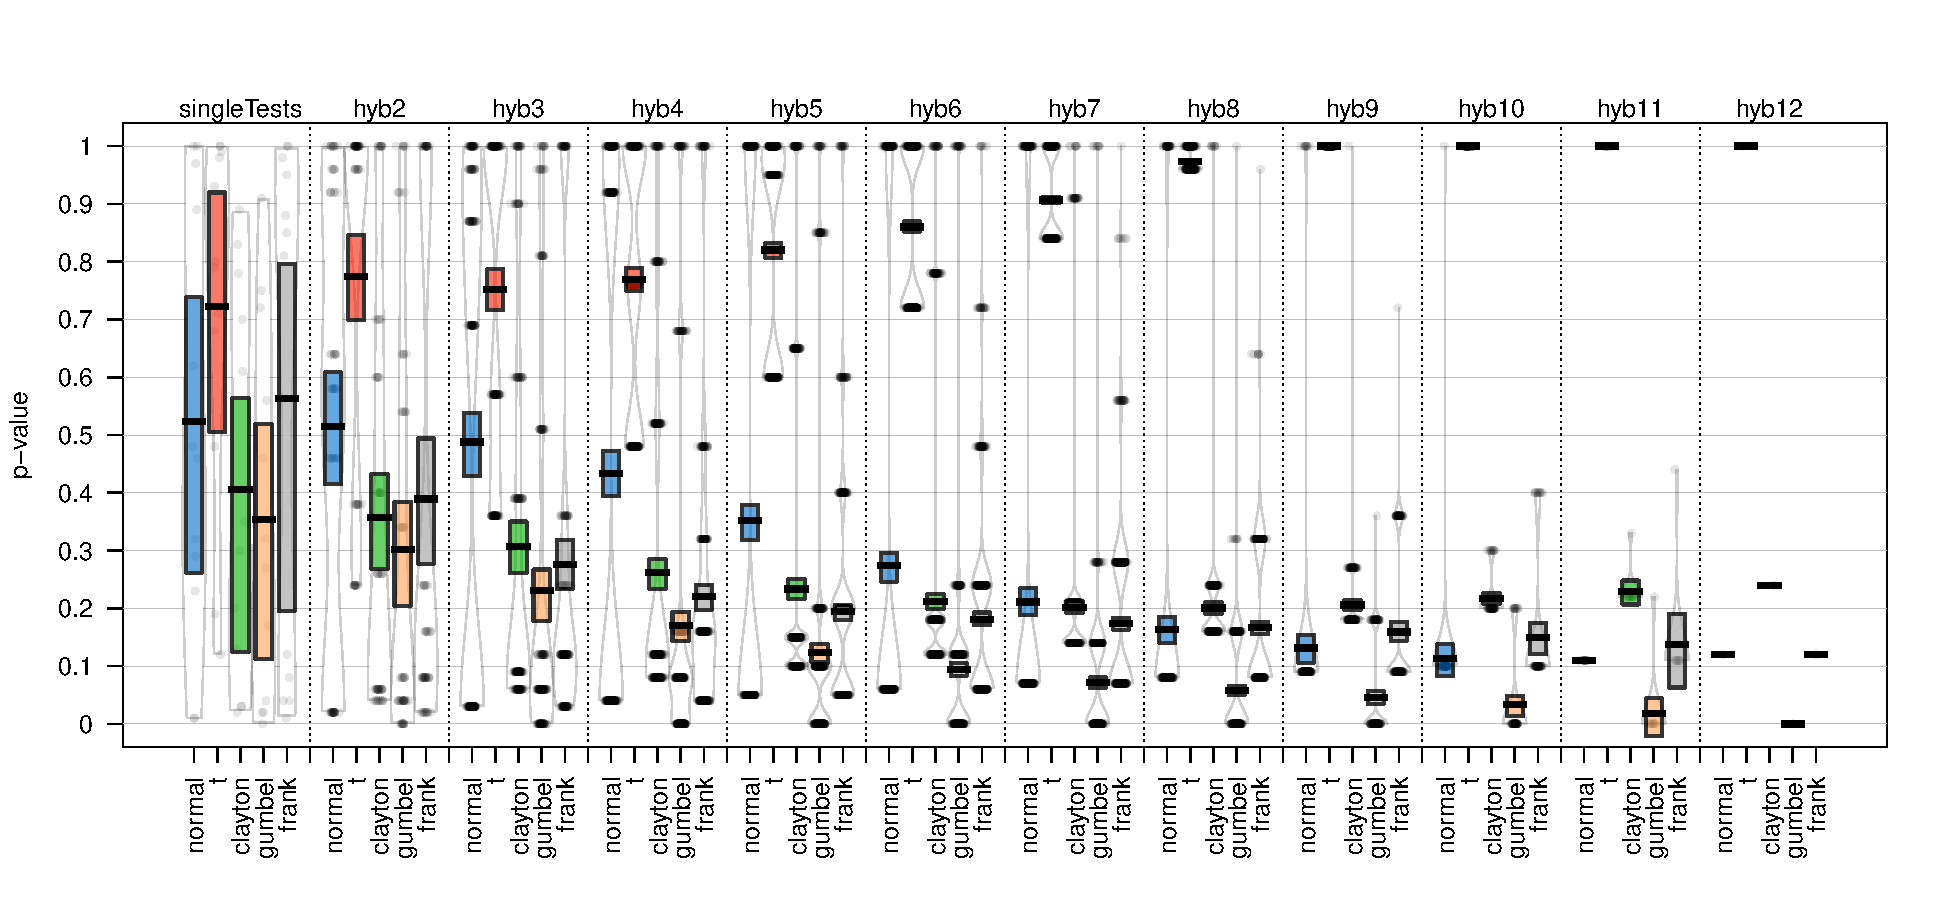
\includegraphics[width=\textwidth]{img/C_BoA_10.pdf}
	\caption{$p$-values of the C/BoA data for 2010.}
	\label{Pirateplot_C_BoA_10}
\end{figure}
\begin{figure}[H]
	\centering
 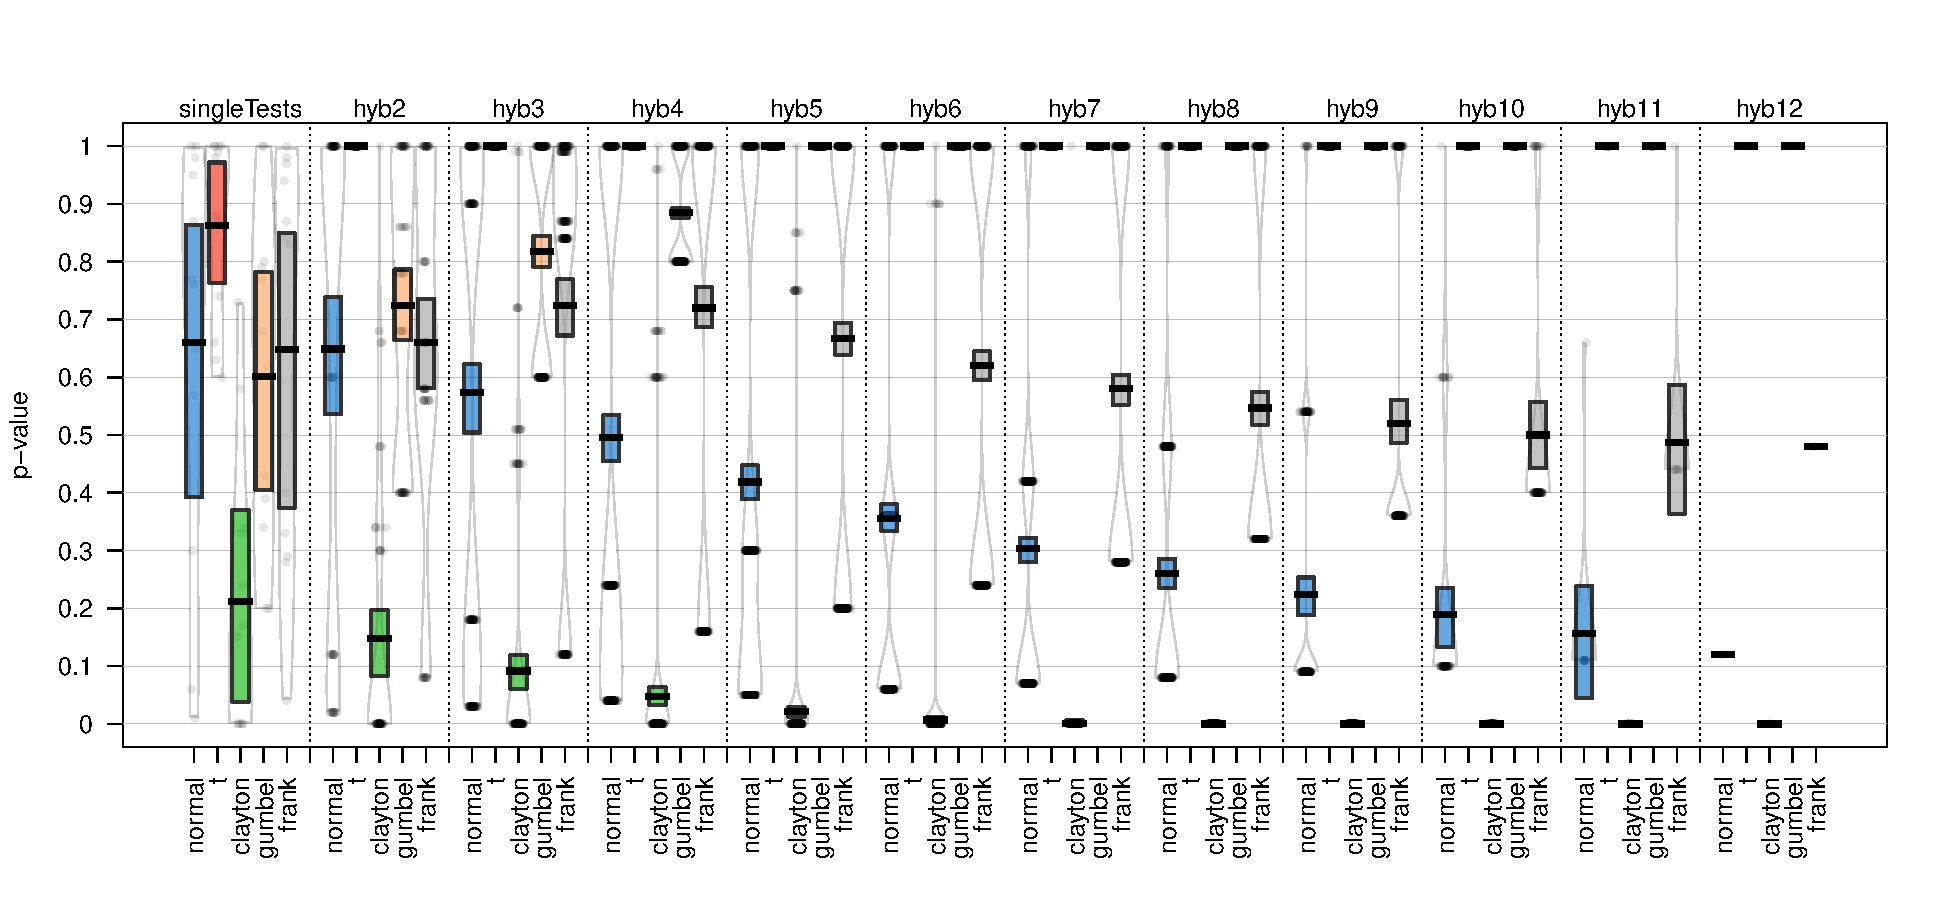
\includegraphics[width=\textwidth]{img/C_BoA_11.pdf}
	\caption{$p$-values of the C/BoA data for 2011.}
	\label{Pirateplot_C_BoA_11}
\end{figure}

\begin{figure}[H]
	\centering
 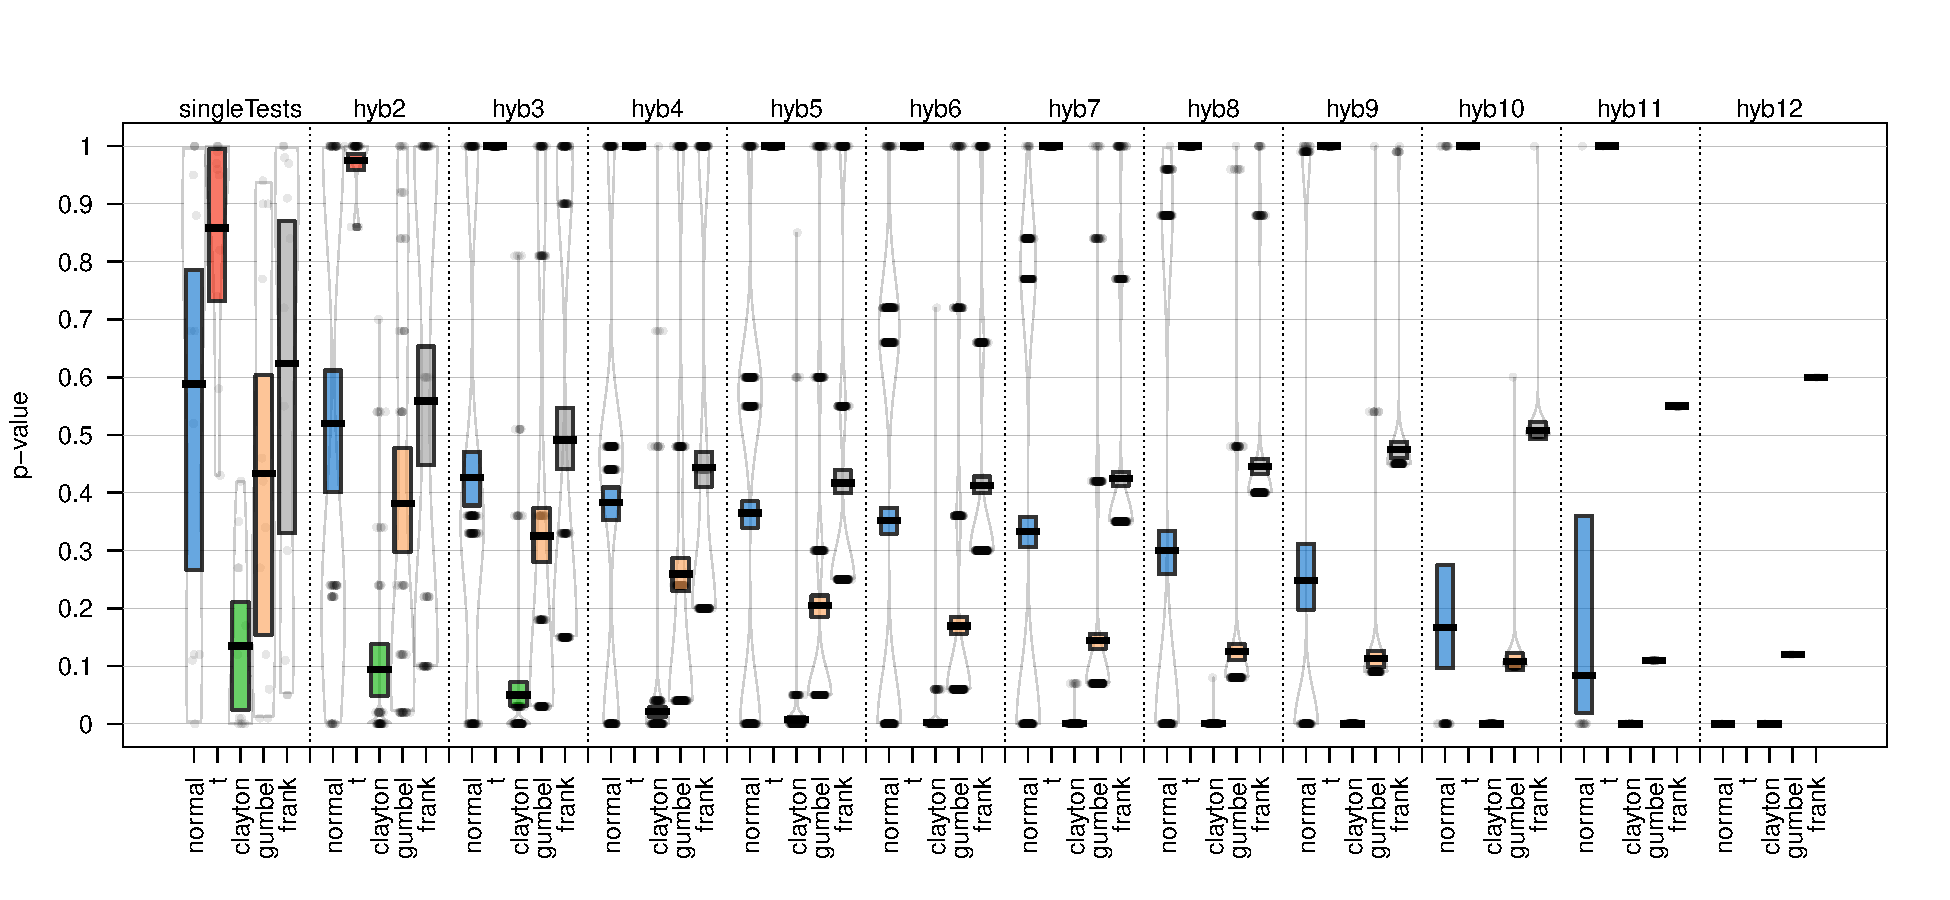
\includegraphics[width=\textwidth]{img/C_BoA_12.pdf}
	\caption{$p$-values of the C/BoA data for 2012. The column \mycolor \protect\code{hyb12} \bk of the $t$-copula is empty, as the $p$-value of the test \protect\code{gofWhite} could not be computed due to instability in the test statistics. For a detailed description of this phenomenon, see \citet{schepsmeier2018package}.}
	\label{Pirateplot_C_BoA_12}
\end{figure}
\end{appendices}

\address{Ostap Okhrin\\
  Chair of Econometrics and Statistics, esp. in Traffic Sciences\\
  Institute of Transportation Economics\\
  Faculty of Transportation\\
  Technische Universit\"at Dresden\\ 
  W\"urzburger Street 35, 01187 Dresden\\
  Germany\\
  \email{ostap.okhrin@tu-dresden.de}}
  
\address{Simon Trimborn\\
  Department of Management Sciences\\
  and School of Data Science\\
  City University of Hong Kong\\
  \mycolor 7-268, Lau Ming Wai Academic Building \bk\\
  Hong Kong\\
  \email{trimborn.econometrics@gmail.com}}

\address{Martin Waltz\\
  Chair of Econometrics and Statistics, esp. in Traffic Sciences\\
  Institute of Transportation Economics\\
  Faculty of Transportation\\
  Technische Universit\"at Dresden\\ 
  W\"urzburger Street 35, 01187 Dresden\\
  Germany\\
  \email{martin.waltz@tu-dresden.de}}

\end{article}

\end{document}
